% Options for packages loaded elsewhere
\PassOptionsToPackage{unicode}{hyperref}
\PassOptionsToPackage{hyphens}{url}
%
\documentclass[
]{book}
\usepackage{lmodern}
\usepackage{amssymb,amsmath}
\usepackage{ifxetex,ifluatex}
\ifnum 0\ifxetex 1\fi\ifluatex 1\fi=0 % if pdftex
  \usepackage[T1]{fontenc}
  \usepackage[utf8]{inputenc}
  \usepackage{textcomp} % provide euro and other symbols
\else % if luatex or xetex
  \usepackage{unicode-math}
  \defaultfontfeatures{Scale=MatchLowercase}
  \defaultfontfeatures[\rmfamily]{Ligatures=TeX,Scale=1}
\fi
% Use upquote if available, for straight quotes in verbatim environments
\IfFileExists{upquote.sty}{\usepackage{upquote}}{}
\IfFileExists{microtype.sty}{% use microtype if available
  \usepackage[]{microtype}
  \UseMicrotypeSet[protrusion]{basicmath} % disable protrusion for tt fonts
}{}
\makeatletter
\@ifundefined{KOMAClassName}{% if non-KOMA class
  \IfFileExists{parskip.sty}{%
    \usepackage{parskip}
  }{% else
    \setlength{\parindent}{0pt}
    \setlength{\parskip}{6pt plus 2pt minus 1pt}}
}{% if KOMA class
  \KOMAoptions{parskip=half}}
\makeatother
\usepackage{xcolor}
\IfFileExists{xurl.sty}{\usepackage{xurl}}{} % add URL line breaks if available
\IfFileExists{bookmark.sty}{\usepackage{bookmark}}{\usepackage{hyperref}}
\hypersetup{
  pdftitle={Finance},
  pdfauthor={Dyrehaugen Web Notebook},
  hidelinks,
  pdfcreator={LaTeX via pandoc}}
\urlstyle{same} % disable monospaced font for URLs
\usepackage{longtable,booktabs}
% Correct order of tables after \paragraph or \subparagraph
\usepackage{etoolbox}
\makeatletter
\patchcmd\longtable{\par}{\if@noskipsec\mbox{}\fi\par}{}{}
\makeatother
% Allow footnotes in longtable head/foot
\IfFileExists{footnotehyper.sty}{\usepackage{footnotehyper}}{\usepackage{footnote}}
\makesavenoteenv{longtable}
\usepackage{graphicx}
\makeatletter
\def\maxwidth{\ifdim\Gin@nat@width>\linewidth\linewidth\else\Gin@nat@width\fi}
\def\maxheight{\ifdim\Gin@nat@height>\textheight\textheight\else\Gin@nat@height\fi}
\makeatother
% Scale images if necessary, so that they will not overflow the page
% margins by default, and it is still possible to overwrite the defaults
% using explicit options in \includegraphics[width, height, ...]{}
\setkeys{Gin}{width=\maxwidth,height=\maxheight,keepaspectratio}
% Set default figure placement to htbp
\makeatletter
\def\fps@figure{htbp}
\makeatother
\setlength{\emergencystretch}{3em} % prevent overfull lines
\providecommand{\tightlist}{%
  \setlength{\itemsep}{0pt}\setlength{\parskip}{0pt}}
\setcounter{secnumdepth}{5}
\usepackage{booktabs}
\usepackage{amsthm}
\makeatletter
\def\thm@space@setup{%
  \thm@preskip=8pt plus 2pt minus 4pt
  \thm@postskip=\thm@preskip
}
\makeatother

\renewcommand\chaptername{}
\usepackage[]{natbib}
\bibliographystyle{apalike}

\title{Finance}
\author{Dyrehaugen Web Notebook}
\date{2022-09-19}

\begin{document}
\maketitle

{
\setcounter{tocdepth}{1}
\tableofcontents
}
\hypertarget{finance}{%
\chapter{Finance}\label{finance}}


\includegraphics{fig/zelda.jpg}

Finance is not production, but it seems to be involved in every aspect of it.

Indeed, under conditions of financial capital abundance,
finance operates not so much as ``a system for the allocation of resources''
than as ``a weapon by which the claims of wealth holders are
asserted against the rest of society''.

Piketty himself gets into some murky waters because his
``Marshallian apparatus'' sees capital ``more as a stock of accumulated savings rather
than a claim on future output''.

Finance is a way to separate foolish retail investors from their hard-earned savings.

\hypertarget{capitalization}{%
\chapter{Capitalization}\label{capitalization}}

\hypertarget{discount-rate}{%
\section{Discount Rate}\label{discount-rate}}

\emph{Fix}

Where did the discount rate come from? The answer: out of thin air. Like the capitalization ritual itself, the discount rate is whatever we define it to be. Capitalists employ the capitalization ritual by ritualistic choosing a discount rate that they deem `proper'.

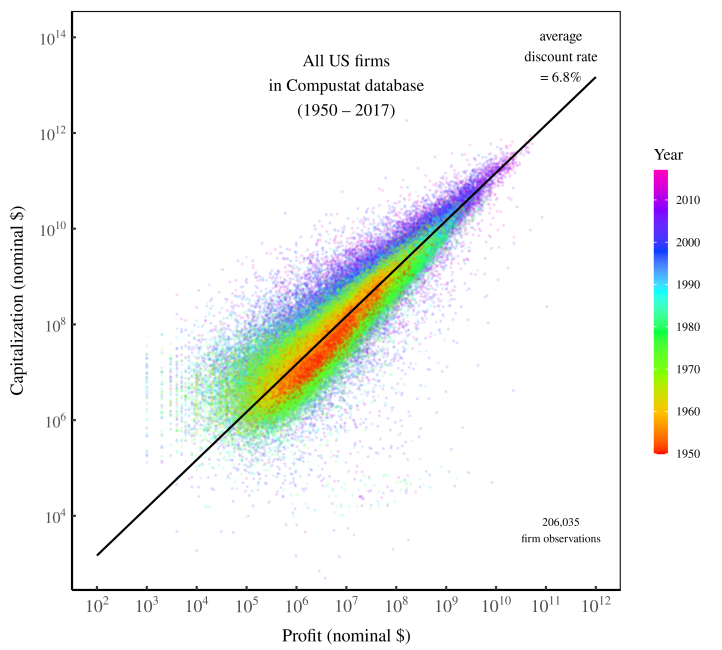
\includegraphics{fig/profit_cap.png}

\emph{Figure: Profit and capitalization of US firms, 1950 -- 2017. Each point represents a US firm. Color indicates the year of observation. The black line shows how capitalization relates to profits for a discount rate of 6.8\% --- the average found in the data. There are about 200,000 observations in total.}

Capitalization is proportional to profit discounted at a rate of 7\%.

Is there something special about the discount rate of 7\%? The answer is yes and no. That rate is special in the sense that it's what US capitalists have deemed to be `proper'. But this rate is banal in the sense that it has no deeper meaning. US capitalists discount at 7\% because that is the norm they have accepted. Gesture the cross. Discount at 7\%. Regularity from ritual.

\begin{quote}
Until the emergence of capitalization in the fourteenth century, {[}the `proper' discount rate was{]} seen as a matter of state decree, sanctioned by religion and tradition, and modified by necessity. The nobility and clergy set the just lending rates as well as the tolerated zone of private divergence, and they often kept them fixed for very long periods of time.
\end{quote}

Today, the `proper' discount rate still has an element of decree. Governments (via central banks) set the benchmark interest rate, which in turn affects the benchmark discount rate on equity.

Far more than just a `monetary phenomena', then, the inflation rate signals instability in the social order. That instability, it seems, translates into capitalists fears about the future. When the price system is more unstable, capitalists discount present income more steeply.

\begin{quote}
The `science of finance' is first and foremost a collective ethos. Its real achievement is not objective discovery but ethical articulation. Taken together, the models of finance constitute the architecture of the capitalist nomos. In a shifting world of nominal mirrors and pecuniary fiction, this nomos provides capitalists with a clear, moral anchor. It fixes the underlying terrain, it shows them the proper path to follow, and it compels them to stay on track. Without this anchor, all capitalists --- whether they are small, anonymous day traders, legendary investors such as Warren Buffet, or professional fund managers like Bill Gross --- would be utterly lost.
\end{quote}

\begin{quote}
Finance theory establishes the elementary particles of capitalization and the boundaries of accumulation. It gives capitalists the basic building blocks of investment; it tells them how to quantify these entities as numerical `variables'; and it provides them with a universal algorithm that reduces these variables into the single magnitude of present value. Although individual capitalists differ in how they interpret and apply these principles, few if any can transcend their logic. And since they all end up obeying the same general rules, the rules themselves seem `objective' and therefore amenable to `scientific discovery'.
\end{quote}

The regularities of corporate finance are majestic in scope. But these regularities stem not from any laws of nature. They are regularities from ritual.

Perhaps the most important question is where this ritual is headed. Does capitalization have a long-term future? Neoclassical economists like William Nordhaus think so. They're happy to apply the capitalization ritual to existential crises like climate change. And the net present value of their calculations tells them (surprise surprise) that we should do essentially nothing. But of course, by applying a heavy discount rate to future income, that is what they assumed in the first place. It's ritualized apathy.

The ritual of capitalization is surrounded by a mystique of `higher truth'. Whenever you encounter such a mystique, it's a good bet that you're dealing with ideology. The point of the `mystique' is to stop you from looking under the ideology's hood.

\href{https://economicsfromthetopdown.com/2021/06/02/the-ritual-of-capitalization/}{Fix (2021) Ritual of Capitalization}

\hypertarget{finance-1}{%
\chapter{Finance}\label{finance-1}}

\hypertarget{global-finance}{%
\section{Global Finance}\label{global-finance}}

\emph{Fitchner Abstract}

The prediction of America's decline is a regularly recurring phenomenon; this also pertains to the
pivotal field of global finance. This article argues that, first we have to consider the United States
together with the other Anglophone countries. The English-speaking countries and territories --
Anglo-America -- have deep common political and socioeconomic roots, of which the unique global Five
Eyes intelligence cooperation is merely one manifestation. In finance, New York and London
(NY-LON) constitute the decision-making core of this transnational formation. Second, to analyse the
highly complex phenomenon of structural power in the globalised international political economy we
have to dig deeper to uncover truly meaningful data. Thus, this article evaluates data for nine central
segments of global finance from around the year 2000 to 2014. Contrary to the assertions of many
declinists, these data show that Anglo-America's dominant structural power has been persistent during
this period. Moreover, four novel visualisations show that the US-UK axis is the fulcrum of the
international financial system. However, contemporary global finance is characterised by a high degree
of latent fragility; significant imbalances, inequalities and contradictions persist and are even likely to
grow, potentially undermining the legitimacy and the stability of the whole system.

\href{https://www.cambridge.org/core/journals/review-of-international-studies/article/perpetual-decline-or-persistent-dominance-uncovering-angloamericas-true-structural-power-in-global-finance/75536FC7435F72FC9AB4968D0509F019}{Fitchner (2021) Anglo-America's power in Global Finance}
\href{pdf/Fitchner_2021_anglo-americas-power-in-global-finance.pdf}{(pdf)}

\hypertarget{money}{%
\section{Money}\label{money}}

\begin{quote}
Money is the alienated essence of man's labour and life; and this alien essence dominates him as he worships it. (Karl Marx)
\end{quote}

\hypertarget{institutional-investors}{%
\subsection{Institutional Investors}\label{institutional-investors}}

\hypertarget{esg-2.0}{%
\subsubsection{ESG 2.0}\label{esg-2.0}}

\emph{Segal}

\textbf{How Institutional Investors Encourage Corporations Bad Behavior}

Wittingly or unwittingly, pensions and endowments' investment strategies aid and abet activities that make the financial system more fragile.

The growing scale of institutions and the large amounts of money they need to deploy into high-risk investments is leading to consolidation among asset managers, higher global debt levels, short-term corporate behavior, and market instability.

Institutions' investment strategies are in conflict with environmental, social, and governance goals to which they are increasingly committing.

Pension funds, insurance companies, sovereign wealth funds and others need to deploy large amounts of capital efficiently because they themselves are so big.

Institutions' only option in many cases is to put billions of dollars to work in the largest public and private companies, Rothenberg explained. That results in companies, for example, taking on unsustainable amounts of debt.

There are incentives to layer on debt, much of which is supplied by capital markets and the shadow banking sector.

Ironically, institutional investors want to integrate ESG into their process, but they also contribute to corporate consolidation and huge debt burdens. Institutional investors are essentially contributing to some of their own problems in the way they allocate capital to leveraged loans, high-yield loans, collateralized loan obligations
and other higher risk products.

All of this adds to global systemic risks.
Unchecked increases in corporate debt result in increased systematic market risk that boomerangs back to investors and their portfolios
Existing approaches like Modern Portfolio Theory and ESG or impact investing frameworks don't focus on these potentially negative effects.

Perversely, as major central banks globally respond to the current crisis with rock bottom interest rates and new rounds of quantitative easing (QE), investors and companies are further incentivized to increase their exposure to high-risk debt and inflated asset valuations --- a situation that leaves society and markets vulnerable to a rise in interest rates or other unplanned challenges

\href{https://www.institutionalinvestor.com/article/b1r9js87jhyn8s/How-Institutional-Investors-Encourage-Corporations-Bad-Behavior}{Segal - Comment - Instititional Investor}

\emph{Rothenburg}

Many of our existing ESG and impact investing frameworks focus on issues at the
portfolio company level, but they do not take into account potential negative
impacts from capital structures and investors' influence in shaping them.
Asset allocation strategies can be in conflict with ESG objectives.

The conflict materializes in various interconnected ways, particularly from
institutional investors' role in increasing global debt levels and
fund manager and corporate consolidation.

For long-term, diversified institutional investors, or ``Universal Owners''
of the market, these dynamics eventually translate into lower financial returns.
For workers and communities, these dynamics translate into
greater precarity and inequality.

Potential solutions focus on diversifying asset allocation to
more regenerative investment structures and asset classes, building an
enabling environment through adjustments to team incentive structures, performance reviews,
benchmarking and valuation methodologies, and field-building.

Over the past decades, institutional investors have migrated up
the risk-return spectrum to asset classes with higher yields.
Investor allocations to private equity (PE), venture capital (VC), private debt (PD),
high yield bonds (HYBs), leveraged loans (LLs), and
collateralized loan obligations (CLOs), for instance,
have been growing steadily in response to a number of trends.
\emph{While such shifts in asset allocation may suit near-term goals,
such as meeting actuarial targets, this institutional allocation to higher risk asset
classes has also meant increased global debt burdens, corporate and
fund manager consolidation, and risk across capital structures,
resulting in fragility for companies, the real economy, and the stability of
financial markets.
The resulting risks are therefore shared not only by investors,
but also governments,workers, and communities alike.}

To optimize leverage ratios, companies may prioritize debt servicing or distributions to investors at the
expense of worker payrolls and benefits. Infrastructure and social infrastructure investments --- such as
power, water, roads, hospitals, nursing homes, housing, and cybersecurity --- might be structured in
such a way that provides access to end-users at unaffordable prices, or of poor quality, in order to meet
investor return expectations and therefore attract capital. Weak capital structures increase the risk of
restructurings or bankruptcies that are detrimental for stakeholders, such as workers. Stakeholders have
increasingly raised concerns about high leverage, coined ``financial engineering,'' particularly in the PE
asset class, for such reasons. 5 Yet studies produced over the past decades, inspired by PE, praise the
discipline of debt, and due to a number of additional factors, high leverage ratios are no longer confined
to the PE asset class and are prolific across public equity markets, as well.

In practice, the negative impacts of weak capital structures are typically being addressed piecemeal
through company-by-company interventions that focus on corporate operations, like a game of whack-
a-mole; but key roots of the problem --- the investment structures themselves --- are left unaddressed.

The unintended negative consequences of highly levered investments have been underexplored when it
comes to ESG and impact investing frameworks and practice. Matters relating to investment structures,
capital structures, leverage ratios, earnings calculations, valuation methodologies, benchmarking
approaches, and resulting asset allocation and portfolio construction are not typically within the realm
of ESG-related responsibilities.

Too much leverage is dangerous for all stakeholders.
While leverage looks like a neutral, bilateral accelerant, it
actually reduces financial resiliency at the very times when it might be most needed.

Systemic inequality has been shown to result in economic decline.

Neither Modern Portfolio Theory (MPT) nor ESG or impact investing frameworks
currently include a focus on potential negative impacts stemming from
investment structures.

Corporate debt burdens and leverage ratios are historically high, covenants are light, and
defaults and bankruptcies are being held at bay by government support
(e.g.~through fiscal and monetary policy) -- which is also funded by debt,
though at the sovereign level.

Corporate funding dynamics have changed since the Global Financial Crisis
(GFC), when banks came under heavy regulation that caused them to
restrict lending to smaller clients.
Capital markets, or the Non-bank Financial Intermediary
(``NBFI'' or ``Shadow Banking'') sector, has stepped in to fill this void.

The financial assets of the NBFI sector amounted to \$200.2 trillion in 2019,
accounting for nearly half of the global financial system in 2019, up from 42\%
in 2008

\emph{How Did We Get Here?}

For the past two decades, institutional asset owners have significantly shifted their overall asset
allocation strategy. Private markets -- including PE, PD, VC, infrastructure, and real estate - as well as LLs,
CLOs, and HYBs, have become much larger percentages of overall portfolios. There are a number of
reasons for these changes, including, but not limited to, ongoing declines in interest rates by major
global central banks, dynamics related to funding ratios of institutional investors such as pension funds,
growing interest in the illiquidity premium of private markets, benchmarking practices, investor
dissatisfaction with public markets, and increased opportunity for NBFIs to provide financing following
banking regulations resulting from the GFC. 16 Private capital assets under management (AUM) in 2019
was approximately US\$6.5 trillion, an increase of over US\$4 trillion over the past ten years.

\emph{Private Equity (PE)}

Investor demand is now so high for PE that many are concerned that the asset class is becoming crowded with capital.

Consolidated capital flows stems from the institutionalization of capital.
Markets have evolved from being dominated by individual investors to
having a large presence of institutional investors.
Institutional investors now hold over 40 percent of
global market capitalization of listed companies.

Institutional investors have sizable portfolios and must invest billions
if not trillions of dollars.
With such large chunks of capital to put to work,
they often find it challenging to invest in smaller fund managers,
smaller companies, and niche investment strategies due to a number of factors,
such as transaction costs.

Even when small deals perform well, which data suggests that they often do,
they are hard to justify because they do not meaningfully move the needle
in terms of overall portfolio returns.

A well-documented negative impact of consolidated capital flows to larger
fund managers is that
smaller, emerging, and innovative fund managers can be starved of capital.

\emph{Institutionalization of Capital}

The consolidation of capital among institutional investors is a double-edged sword. On the one hand,
institutions offer individual investors professional money management with multi-disciplinary staff and
robust internal infrastructure capable of constructing well-diversified portfolios. Size and scale can also allow
large allocators to influence corporate governance of portfolio companies, as well as negotiate more
attractive terms with fund managers. It is arguable that fees overall are reduced through these dynamics, and
strong ESG practices can be better advocated for. On the other hand, since large institutions need to put
significant amounts of capital to work, they often allocate to the largest managers and companies, thereby
resulting in consolidation of power, profit, influence, and opportunity among a shrinking pool of asset
managers and companies. 53 In order for large institutional investors to act as responsible Universal Owners
and effectively manage systematic risk, it will be critical for them to evaluate their asset allocation practices
for unintended negative consequences that not only impact the real economy, but also markets and their
long-term portfolios.

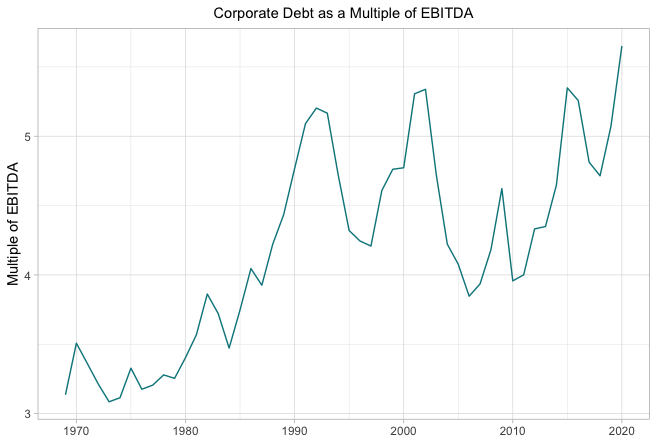
\includegraphics{fig/corporate_debt_ebitda.png}

This high-risk debt is not limited to private companies. A recent Forbes article highlights how, ``some of
the biggest firms in the United States\ldots{} have binged on low interest debt. Most of them borrowed more
than they needed, often returning it to shareholders in the form of buybacks and dividends. They also
went on acquisition sprees.''

From the corporate perspective, historically cheap credit due to low interest rates is attractive,
particularly when combined with the current tax deductibility of interest expense, studies suggesting
that highly leveraged capital structures do not negatively impact stock prices, and arguments that debt
adds discipline to corporate management. Yet debt and common uses of funds can increase risk for
other stakeholders. M\&A has been shown to contribute to corporate consolidation which can stifle
SMEs, innovation, suppliers, the quality and affordability of goods and services, labor's bargaining
power, and diversification for institutional investors. There is significant literature that explores
negative impacts of share buybacks in public companies, given the links with high executive
compensation and that cash paid to executives and shareholders can deter from reinvestment in the
company, the quality of goods and services, and the workforce. In PE-backed companies, high leverage
from acquisitions and dividend recapitalizations can push companies to cut costs related to quality jobs
and jeopardize the quality and affordability of goods and services.

As central banks around the world doubled down on low interest rates and QE, investors responded by
increasing portfolio allocation to higher risk and yielding asset classes.

The combination of QE and low interest rates with corporate consolidation and high
inequality may well be creating challenges to long-term economic growth,
as well as introducing
potential drivers of instability for aggregate demand.

\href{https://papers.ssrn.com/sol3/papers.cfm?abstract_id=3820316}{Rothenberg (2021) ESG 2.0 - Measuring \& Managing Investor Risks Beyond the Enterprise-level}
\href{Rothenberg_2021_ESG2.pdf}{(pdf)}

\hypertarget{central-banks}{%
\section{Central Banks}\label{central-banks}}

In managing our economy with disembedded measures of wealth,
the world's central bankers are effectively agents of the sustainability crisis. They may not
wish to be unsustainable by personal inclination, but they certainly are by professional
obligation because of how they are duty-bound to act.
An entirely foreseeable response to the climate emergency is that people in wealthier
countries may choose to pare back their consumption of non-essentials. Certainly, not
everyone has the luxury to do this, but the obvious solution of ``buying less stuff'' has become
an articulated idea in wealthy countries. ``Flight shaming'' and ``consumption shaming'' are new
memes. Articles in multiple UK newspapers have challenged readers to see if they can go a
year without buying any new clothes, contravening the media's normal practice of generally
trying to coax the economy along. (It buoys the advertising revenue).
Such behaviours would amount to a direct hit on GDP in developed countries, where personal
consumption can represent two-thirds of the total. Critically, any such reduction in
consumption will likely show up as a deflationary decline in economic activity that the world's
central banks are on hair-trigger alert to prevent. The large and powerful financial
bureaucracy stands ready to provide immediate stimulus to any perceived flagging of
measured economic activity.
Hence, the arrangement most populations in the world currently live under is that should they
collectively choose to buy less, more money will be printed until they have changed their
mind. Effectively, our exhausted ecosystem is gasping for a lull in measured economic activity
that our financial authorities are pledged to never let happen.

\href{pdf/Austin_2021_Pigou_\%20and_the_dropped_stitch_of_economics_RWER95.pdf}{Duncan Austin: Pigou and the dropped stitch of economics RWER95 (pdf)}

\hypertarget{central-bank-independence}{%
\subsection{Central Bank Independence}\label{central-bank-independence}}

\textbf{Market Neutrality}

\emph{Klooster Abstract}

Monetary policy operations in corporate security markets confront central
banks with choices that are traditionally perceived to be the prerogative of
governments. This article investigates how central bankers legitimise
corporate security purchases through a comparative study of the
European Central Bank (ECB) and the Swiss National Bank (SNB). As we
show, central bankers downplay the novelty of corporate security
purchases by relying on familiar pre-crisis justifications of Central Bank
Independence. Citing an ideal of `market neutrality', central banks
present corporate security purchases as pursuing a narrow objective of
price stability and obfuscate their distributive consequences. In this way,
central bankers depoliticise corporate security purchases: they reduce
the potential for choice, collective agency, and deliberation concerning
both the pursuit of corporate security purchases and the choices made
in implementing these policies. We also describe the undesirable
democratic, social and environmental dimensions of these practices,
which we propose to address through enhanced democratic
accountability.

\emph{Klooster Memo}

The past decades saw central banks acquire considerable independence from democratic institutions
(McNamara 2002, Singleton 2010). Governments justified their decision to delegate monetary policy
by relying on a narrow conception of monetary policy. This conception focuses on the setting of short
term interest rates to achieve a long-term objective of stable price levels. A crucial element in the
justification of central bank independence is the idea that monetary policy is an apolitical, technical
area of policymaking (Marcussen 2009). The loss of democratic control that results from the creation
of an independent central bank was also thought to be minimal, because distributive choices would
remain with elected governments, who both decided on the central bank mandate and retained the
use of fiscal instruments to achieve their distributive objectives. In this way, governments depoliticised
monetary policy in the sense of reducing the potential for choice, collective agency, and deliberation
around the use of monetary policy

The Global Financial Crisis (GFC) led central bankers to move far beyond the narrow task assigned
to them under the traditional justification of Central Bank Independence (CBI)
To rescue a global financial system on the brink of collapse, central bankers assumed new roles as lenders and market makers of last resort.

Central bankers, meanwhile, are openly concerned that the use of unconventional tools threatens
their independence.
When independent regulatory agencies extend their power, political authorities often seek to regain
control.
Central bankers, accordingly, try to counteract repoliticisation and these efforts
shape their policies.

To investigate the simultaneously occurring processes of politicisation and depoliticisation
we investigate how central bankers relate to the political dimensions of their
new unconventional policies.

\href{https://www.tandfonline.com/doi/epub/10.1080/13563467.2019.1657077?needAccess=true}{Klooster (2021) The Myth of Market Neutrality}
\href{pdf/Klooster_2021_Myth_of_Market_Neutrality.pdf}{(pdf)}

The new exogenous money is exogenous transition shocks in the climate change debate.
Fortunately, Bank of England cannot hide behind that rock because of their new climate mandate.

Remember, Mark Carney's `tragedy of the horizons' speech identified two main risks of climate crisis:
- physical risks (climate events)
- transition risks - from green policies to accelerate transition to low-carbon

Now, central banks are confronted with an unpleasant conundrum that reveals the deeply political nature of their operations:
greening monetary policy (collateral, unconventional bond purchases) means endogenous transition risks

So, in a have your cake and eat it moment, there is a growing tendency in central bank communities to pretend that all transition risks come from the fiscal side (carbon pricing)

It wouldn't be surprising to find the exogenous transition shocks approach in the ECB's monetary policy strategy review, despite \citet{Lagarde}
and other's recognition that central banks cannot longer hide behind the `market neutrality' argument.

\href{https://twitter.com/DanielaGabor/status/1384837864412917765}{Gabor (Twitter)}

\hypertarget{sovereign-debt-held-by-central-banks}{%
\subsection{Sovereign Debt held by Central Banks}\label{sovereign-debt-held-by-central-banks}}

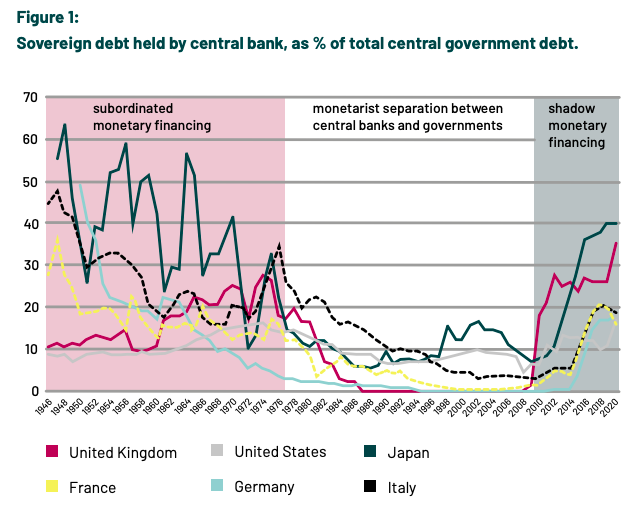
\includegraphics{fig/sovereign_debt_held_by_central_banks.png}

\href{https://transformative-responses.org/the-project/next-generation-central-banking-climate-change-inequality-financial-instability/}{Gabor (2021) Revolution without revolutionaries: Interrogating the return of monetary financing}

\hypertarget{financial-stability}{%
\subsection{Financial Stability}\label{financial-stability}}

\hypertarget{climate-risk}{%
\subsubsection{Climate Risk}\label{climate-risk}}

\hypertarget{bis-recommendations}{%
\paragraph{BIS Recommendations}\label{bis-recommendations}}

This report provides an overview of conceptual issues related to climate-related financial risk
measurement and methodologies, as well as practical implementation by banks and supervisors.

The report contains five key findings:
First, climate-related financial risks have unique features, necessitating granular and
forward-looking measurement methodologies.

Second, to date, measurement of climate-related financial risks by banks and supervisors
has centred on mapping near-term transition risk drivers into counterparty and portfolio exposures.

Third, banks and supervisors have predominantly focused on assessing credit risk, as they
advance in applying methods to translate climate-related exposures into categories of financial risk.

Fourth, while banks and supervisors remain at an early stage of translating climate-related
risks into robustly quantifiable financial risk, work continues to gather pace

Fifth, key areas for future analytical exploration relate to measurement gaps in data and
risk classification methods, as well as methodologies suitable for assessing long-term climate
phenomena not always of a standard nature.

\href{https://www.bis.org/bcbs/publ/d518.htm}{BIS (2021) Climate Risk}
\href{pdf/BIS_2021_Climate_Risk.pdf}{(pdf)}

\hypertarget{index-providers}{%
\section{Index Providers}\label{index-providers}}

\emph{Fitchner}

A silent revolution is happening in investing. It is a paradigm shift that will have a profound impact on corporations, countries and pressing issues like climate change.
A silent revolution is happening in investing. It is a paradigm shift that will have a profound impact on corporations, countries and pressing issues like climate change.
In 2019 there was a watershed in the history of finance. In the United States, the total value of actively managed funds was surpassed by passive funds. Globally, passive funds crossed US\$10 trillion (£7.7 trillion), a five-fold increase from US\$2 trillion in 2007.

This seemingly unstoppable ascent has two main consequences.

First, corporate ownership has become concentrated in the hands of the ``big three'' passive asset managers: BlackRock, Vanguard and State Street. They are already the largest owners of corporate America.

The second consequence relates to the companies that provide the indices that these passive funds follow. When investors buy index funds, they effectively delegate their investment decisions to these providers. Three dominant providers have become increasingly powerful: MSCI, FTSE Russell and S\&P Dow Jones Indices.

A silent revolution is happening in investing. It is a paradigm shift that will have a profound impact on corporations, countries and pressing issues like climate change. Yet most people are not even aware of it.

In a traditional investment fund, the decisions about where to invest the capital of the investors are taken by fund managers. They decide whether to buy shares in firms like Saudi Aramco or Exxon. They decide whether to invest in environmentally harmful businesses like coal.

Yet there has been a steady shift away from these actively managed funds towards passive or index funds. Instead of depending on a fund manager, passive funds simply track indices -- for example, an S\&P 500 tracker fund would buy shares in every company in the S\&P 500 in order to mirror its overall performance. One of the great attractions of such funds is that their fees are dramatically lower than the alternative.

In 2019 there was a watershed in the history of finance. In the United States, the total value of actively managed funds was surpassed by passive funds. Globally, passive funds crossed US\$10 trillion (£7.7 trillion), a five-fold increase from US\$2 trillion in 2007.
¿Le gusta lo que lee? ¿Quiere más?

This seemingly unstoppable ascent has two main consequences. First, corporate ownership has become concentrated in the hands of the ``big three'' passive asset managers: BlackRock, Vanguard and State Street. They are already the largest owners of corporate America.

The second consequence relates to the companies that provide the indices that these passive funds follow. When investors buy index funds, they effectively delegate their investment decisions to these providers. Three dominant providers have become increasingly powerful: MSCI, FTSE Russell and S\&P Dow Jones Indices.

With trillions of dollars migrating to passive funds, the role of index providers has been transformed.

In the past, index providers only supplied information to financial markets. In our new age of passive investing, they are becoming \emph{market authorities}.
Deciding who appears in the indices is not just something technical or objective. It involves some discretion by the providers and benefits some actors over others. By determining which players are included on the list, setting the criteria becomes an inherently political activity.

The three dominant index providers' income mainly derives from the funds replicating their indices, since they have to pay royalties for the privilege.
MSCI, FTSE Russell and S\&P Dow Jones will increase their role as \emph{a new kind of de facto
global regulators}.

This tightly interlinked group of three giant passive fund managers and three major index providers will largely determine how corporations tackle climate change. The world is paying little attention to the judgements they make, and yet these judgements look highly questionable. If the world is truly to get to grips with the global climate crisis, this constellation needs to be far more closely scrutinised by regulators, researchers and the general public.

\href{https://theconversation.com/three-financial-firms-could-change-the-direction-of-the-climate-crisis-and-few-people-have-any-idea-131869}{Fitchner in The Conversation}

\emph{Petry}

Since the global financial crisis, there is a massive shift of assets towards index
funds. Rather than picking stocks, index funds replicate stock indices such as the
S\&P 500. But where do these indices actually come from? This paper analyzes the
politico-economic role of index providers, a small group of highly profitable firms
including MSCI, S\&P DJI, and FTSE Russell, and develops a research agenda from an
IPE perspective. We argue that these index providers have become actors that exer-
cise growing private authority as they steer investments through the indices they
create and maintain. While technical expertise is a precondition, their brand is the
primary source of index provider authority, which is entrenched through network
externalities. Rather than a purely technical exercise, constructing indices is inher-
ently political. Which companies or countries are included into an index or excluded
(i.e.~receive investment in- or outflows) is based on criteria defined by index pro-
viders, thereby setting standards for corporate governance and investor access.
Hence, in this new age of passive asset management index providers are becoming
gatekeepers that exert de facto regulatory power and thus may have important
effects on corporate governance and the economic policies of countries.

Index mutual funds have been available since the late 1970s and the first ETFs
have been launched in the early 1990s. However, investors shunned them for a long
time. But after the global financial crisis growth of index funds has accelerated mas-
sively.

An unprecedented
money mass-migration from active to passive funds, which is rational as most
actively managed funds are unable to beat broad market indices over longer time
periods but charge high fees.

One crucial, yet largely unstudied element of this new era is that
index funds effectively delegate their investment decisions to index providers. Index
providers are the firms that create and maintain the indices on which passive funds
rely and to which asset managers have to pay fees if they use them.

Similar to passive asset management, which is dominated by the `Big Three' of
BlackRock, Vanguard, and State Street (Fichtner et al., 2017), the global index pro-
vider industry is very concentrated. Just three firms, MSCI, S\&P Dow Jones Indices
(DJI) and FTSE Russell, hold a combined market share of almost 80\%.

While global index revenues totaled a record US\$2.7 billion in 2017,
their profit margins that stand out as exceptionally high.
MSCI reports an operating margin of over 60\% for its index segment in 2018.
Index providers operate in an oligopolistic industry,
which has high barriers to competition.

During the last decade the big index providers have had
much higher growth than most other financial companies, especially banks.

Index providers today occupy a position of growing
private authority, with decision-making and standard-setting capabilities that are
consequential in the global political economy. In the past, their indices primarily
served informational purposes. An index such as the S\&P 500 or the Nikkei was
primarily a numerical representation of a particular stock market. Indices served as
benchmarks against which analysts could gauge the performance of stocks. While
the decisions of index providers had some impact on actively managed funds, the
rise of passive investing transformed their role in a significant way. Today, they de
facto steer capital with their indices as inclusions of firms or countries to an
index can lead to inflows of billions of US\$ while exclusions can cause large quasi-
automatic outflows. Constructing indices is therefore not a purely technical exer-
cise. Index providers have significant discretion in devising their methodologies.

The methodology of the pivotal S\&P 500
index was changed at least eight times between 2015 and 2018. Underlying their
seemingly technical exercise are decisional discretion and normative assumptions
about `good' corporate governance and `free' markets. Index providers therefore
play a role as standard-setters: their notions on what constitutes good corporate
governance at the level of the firm and a favorable investment environment at the
level of (national) markets helps or hinders firms and countries in attracting cap-
ital, essentially deciding what is investment-worthy in global financial markets.
This combination of standard-setting and legitimate decision-making power means
that index providers have gained a position of private authority in capital markets
with profound politico-economic consequences.
Today index providers have become important counterparts for states.

Index providers increasingly are
to equity markets what credit rating agencies are to bond markets, crucial
`coordination service firms' that exercise private authority and effectively
set standards for the behavior of other firms and even countries

Their new authority was not delegated from
the public sphere, but gradually emerged as part of a transformation of the index
provider industry -- from primarily supplying information about markets to
becoming private authorities that are able to set standards on corporate governance and
steer international capital flows.

Take for example FTSE Russell, S\&P DJI and
MSCI's emerging market indices; the index providers' recent decision to include
countries such as China and Saudi Arabia to their indices is expected to result in a
`seismic shift' of over US\$120 billion in active and passive fund flows by 2020.

Indices act as `prisms' through which fund managers view the investible world.

Financial market indices are far from objective.

They represent `deliberate decisions'
made by index providers as every index is a managed portfolio whose composition
is decided by the respective index provider.

While these
simplified numerical representations might seem objective and technical, they are
actually based on complex and (often contested) normative values. Moreover, proc-
esses of index production are inherently subjective activities.

Standard-setting is always political.

\emph{Distance Governance}

Indices and indicators have a governing effect on those that are being evaluated,
incentivizing the individuals, companies or states that are being assessed
to comply with the norms underlying those numerical representations,
as better performance has positive ideational and material effects,
enabling a form of `governance from a distance'

Critical gatekeepers that exert de facto regulatory power.

The emergence of private authority through the retreat of the state,
which provided a space for private actors such as firms to exercise authority.

Questions such as the public regulation of index providers.

Private authority is inherently relational, produced and
reproduced through ongoing interactions between the authority and non-authorities,
where the formers' decisions are considered as legitimate by the latter

Rather than coercion or self-interest, legitimacy is a `normative belief
by an actor that a rule or institution ought to be obeyed' and is based on how the
authority is `perceived' by non-authoritarian actorsRather than coercion or self-interest,
legitimacy is a `normative belief by an actor that a rule or institution ought to be obeyed'
and is based on how the authority is `perceived' by non-authoritarian actors.

Three conditions for index provider authority.
First of all, technical expertise to construct an index is a necessary -- but not sufficient.
Second condition; crucial for index provider authority is their brand recognition,
or more specifically the trust that the international investment community puts in their brands.
`Authority is socially constructed' and is ultimately based on
trust, which in turn is based on reputation.
The big three index providers are `brand managers'
: `at the end of the day, those products are homogeneous and exchangeable.
It's like water, there are small differences why Evian is more expensive {[} \ldots{} {]}.
Those are minimal differences, but the price tags are very different!
A third condition that underpins index provider authority lies in a set of net-
work externalities that reinforce the authority of the major index providers. As first
movers they have in effect `captured' different national (e.g.~S\&P 500 or FTSE 100)
and regional (Euro Stoxx 50) market segments with their indices.
These network externalities entrench the authority
that leading index providers derive from their brands. With these three conditions in
place, index providers have become private authorities in financial markets.

The authority of rating agencies developed within and was enabled by changing socio-
economic structures, i.e.~the growth of capital markets and the decline of banks as
allocators of credit, which created a demand for rating agencies' services for the
functioning of the then disintermediated structure of finance.

Authority is best understood as an effect of these circumstances, rather than as an entity or a
characteristic of an actor or institution' and `its existence is therefore not func-
tional, {[} \ldots{} {]} but always contingent on time, place, and circumstance.

Indices had at least some influence on asset managers as an
deviation from the relevant index could be conceived as a kind of risk management
metric.
However, indices only loosely anchored the asset allocation as most fund
managers had the discretion to choose both the degree of replicating the index as
well as the time period for doing so.

Changed fundamentally with the rise of passive investing in the mid-2000s.
Index providers began to influence capital flows in an immediate and comprehensive way.
Being a central
component of the index funds ecosystem conferred them -- gradually and only as a
side-effect of their business model -- a position of growing private authority in
financial markets.

The money mass-migration
towards passive investments, which significantly increased the nascent authority
of index providers as evermore funds directly tracked their indices. Whereas in
the past indices only loosely anchored fund holdings around a baseline, now they
had an instant, `mechanic' effect on the holdings of passive funds, `steering' cap-
ital flows. Increasingly, investments were not actively managed by fund managers
but passively invested into index mutual funds and ETFs

This makes sense as the vast
majority of actively managed funds have not been able to beat benchmark indices
over longer periods of time, while charging substantially higher fees than index
funds.

In order to track the performance of `the market', passively
managed funds replicate stock market indices such as the S\&P 500 or the MSCI
World. Rather than trying to generate `alpha' and outperform the market by pick-
ing stocks, these passively managed funds aim to generate `beta', simply replicat-
ing the performance of specific stock markets while minimizing fees.

By investing in an index, passive investors delegate decision-making about
where to invest to index providers. Index investing thus represents a form of
`delegated management' and every discretionary decision by index providers has a
`flow through effect on the investor's portfolio'

A substantial proportion of equity funds that officially are actively managed
funds (and therefore charge higher fees than index funds) but actually do not devi-
ate much from their benchmark indices. This is referred to as `closet indexing' or
`index hugging', and it is estimated that in the EU between 5-15\% of all equity
funds could fall into this category (ESMA, 2016). Therefore, the rise of passive
management also increases the authority of index providers vis- a-vis active man-
agement because by steering evermore passive capital index decisions now mechan-
ically move ever larger parts of the markets, creating a `pull effect' that actively
managed funds need to follow

Hedge funds and sovereign wealth funds (SWFs) generally have low degrees of rep-
licating indices (one exception is the Norwegian SWF, which almost invests like a
global ESG 5 index fund) and are fully discretionary to follow any index modifica-
tion.

Indices no longer merely measure markets. They move them.

Far from simply
providing information on `the market', index providers now offer a variety of cus-
tomized branded products, by either tweaking existing benchmarks or repackaging
proprietary trading strategies into indices which enable the functioning of (passive)
asset management capitalism.

The relationship between index providers and asset managers is intriguing. On
the one hand, asset managers depend on the large index providers to create their
products that are attractive to investors. On the other hand, they have an interest
to reduce the fees they have to pay for using indices. In theory, there are two ways
for competition to emerge in the index industry: through new index providers and
through self-indexing by asset managers. However, both have so far not been able
to break the oligopolistic market structure.

It is further difficult for challenger indices to gain benchmark status as network
externalities entrench the authority of the big index providers.

Index providers not only decide to include particular firms, they
also make decisions on in- and exclusions of entire markets, steering capital with
important politico-economic implications for states.

While many indices are strictly rule-based and thus only influence companies indirectly,
some indices -- including the S\&P 500, the world's most-tracked index -- have com-
mittees that make discretionary, less rule-based decisions.
While the majority of inclusions is rather mechanical
and influence is indirect, it is not uncommon that index decisions target individual
firms to set a `precedence' on a particular issue that then gets incorporated into
existing methodologies.

It has become standard practice for the majority
of key global stock indices to use only the market capitalization of firms for calcu-
lating the weight of companies. Market capitalization primarily derives from the
(future) profits of corporations. Even though that has changed somewhat in the
last decades, profit maximization is still not the exclusive goal of corporations from
countries such as France, Germany and Japan.

\emph{`reluctant regulators'}

`We're not activists. We're setting the minimum standards
that investors generally will accept, and our role is to build consensus amongst that
investor community as to what that minimum standard should be'.

The three big index providers are therefore best
seen as consensus-building agents that aggregate their own interests with those of
asset managers from developed economies, i.e.~mainly from Anglo-
American countries.

Index providers have become de facto private standard-setters over corporate governance.

By reclassifying individual countries, index providers effectively redraw the borders of
markets. Index providers set out the criteria that decide which countries are
`investment-worthy'.

Index providers decide whether to include countries
into their indices and whether to classify them as `frontier', `emerging' or
`developed' markets. 8 By additionally putting countries on watchlists for such inclu-
sions, exclusions or reclassifications, index providers create incentives for states to
comply with their rules.

MSCI in effect controls the definition of which countries
are ``emerging markets.
Criteria are set out in MSCI's Market Classification Framework, com-
prising three elements: economic development; size and liquidity; and investor
access. Economic development is not crucial as a criterion, neither are the size and
liquidity requirements (only 2-5 companies need to meet minimum requirements).
Investor access is the dealmaker/breaker for country classifications, and it is on this
that most indexing decisions are based

While index
decisions about company inclusions are often more indirect and not targeted at indi-
vidual companies, in the case of country reclassifications index providers take a much
more proactive role. As the following cases demonstrate, these deci-
sions have enormous consequences for states and their national stock markets.

MSCI has a quasi-regulatory function -- `even though MSCI is not a regulator, companies need
to abide, to respect their rules'.

\href{https://www.tandfonline.com/doi/full/10.1080/09692290.2019.1699147}{Petry (2021) Steering Capital}
\href{pdf/Petry_2021_Steering_Capital.pdf}{(pdf)}

\hypertarget{hedge-funds}{%
\section{Hedge Funds}\label{hedge-funds}}

In the midst of a global crisis, the hedge fund has prospered. The top fifteen hedge-fund managers earned an estimated \$23.2 billion last year, according to Bloomberg. Chase Coleman, the forty-five-year-old founder of Tiger Global Management, led the way, hauling in more than three billion for himself. The Financial Times took a more democratic view of the phenomenon, noting that the top twenty ``best-performing hedge fund managers of all time'' had provided more than sixty-three billion dollars for their investors during the coronavirus-driven market turmoil, ``making it the industry's best year of gains in a decade.''

Given the supremacy of hedge funds, it was both satisfying and terrifying to observe the recent boom and bust in the value of GameStop, a run driven by small-time speculators. Several hedge funds lost extraordinary amounts of cash---as in billions and billions of dollars---on financial derivatives.

Those who work at hedge funds are diligent about keeping who they are and what they do obscured behind a wall. Secrecy is intrinsic to the job description---for a hedge is a wall.

\href{https://www.newyorker.com/culture/culture-desk/a-brief-history-of-the-hedge-fund}{Kaufman in New Yorker: History of Hedge}

\hypertarget{the-wall-street-consensus}{%
\section{The Wall Street Consensus}\label{the-wall-street-consensus}}

\begin{quote}
Washington Consensus and structural adjustment is good for you,
especially if it helps you avoid US bombing!
\end{quote}

\emph{Gabor}

The Wall Street Consensus is an elaborate effort to reorganize development interventions around partnerships with global finance. The UN's Billions to Trillions agenda, the World Bank's Maximizing Finance for Development or the G20's Infrastructure as an Asset Class update the Washington Consensus for the age of the portfolio glut, to `escort' global (North) institutional investors and the managers of their trillions into development asset classes. Making development investible requires a two‐pronged strategy: enlist the state into risk‐proofing development assets and accelerate the structural transformation of local financial systems towards market‐based finance that better accommodates portfolio investors. Ten policy commandments forge the `de‐risking state'. They create a safety net for investors in development assets, protecting their profits from demand risks attached to commodified infrastructure assets; from political risks attached to (progressive) policies that would threaten cash flows, including nationalization, higher minimum wages and, critically, climate regulation; and from liquidity and currency risks. These risks are transferred to the balance sheet of the state. The new `development as de‐risking' paradigm narrows the scope for a green developmental state that could design a just transition to low‐carbon economies.

\textbf{De-risking Wall Street}

\begin{quote}
`\ldots.we have to start by asking routinely whether private capital,
rather than government funding or donor aid, can finance a
project. If the conditions are not right for private investment, we
need to work with our partners to de-risk projects, sectors, and
entire countries'.
(Jim Yong Kim, World Bank Group President (2017))
\end{quote}

\emph{Washington Consensus}

\begin{quote}
Anchored in the work of John Williamson (1990, 1993),
the Washington Consensus outlined ten policy areas that would set countries on firm
market foundations, under a `holy Trinity' of macroeconomic \emph{stabilization} through
lower inflation and fiscal discipline; \emph{liberalization} of trade and capital flows, of
domestic product and factor markets; and \emph{privatization} of state companies.
\end{quote}

\emph{Financial globalization} sets the particular context in which
`international development' is pursued in the 21 st century.
The new development mantra, spelled out in the \emph{Billions to Trillions} agenda, the World
Bank's \emph{Maximising Finance for Development}, or the G20 \emph{Infrastructure as an Asset
Class}, aims to create investable development projects that can attract global investors
and orient their trillions into financing the SDG (Social Development Goals) ambitions.

For instance, at the 2017
launch of the Maximising Finance for Development, the World Bank promised global
investors \$12 trillion in market opportunities that include ``transportation,
infrastructure, health, welfare, education', minted into bankable/investible projects via
public-private partnerships (PPPs). These are long-term contractual arrangements
through which the private sector commits to finance, construct and manage public
services as long as the state, with multilateral development bank support via blended
finance, shares the risks to guarantee payment flows to PPP operators and investors.

This shift in the development agenda can be conceptualized as the Wall Street
Consensus, an emerging \emph{Development as Derisking} paradigm that reframes the (Post)
Washington Consensus in the language of the Sustainable
Development Goals, and identifies global finance as the actor critical to achieving the
SDG.

\emph{Financialisation of development} - strategies to `escort' financial capital
into derisked asset classes.

In the age of institutional investors
and asset managers that move capital across border via portfolio flows, (subordinated)
financialisation is no longer confined to the balance sheet of banks and non-financial
corporations, but becomes a state-mediated project of constructing new development
asset classes.

The WSC is an attempt to re-orient the institutional mechanisms of
the state towards protecting the political order of financial capitalism --
against climate justice movements and Green New Deal initiatives.

Development as derisking starts with the question `how to make projects bankable', or
how to construct investible development asset classes.

Making development `investible' requires a two-pronged strategy: (a) enlist the state
into derisking development asset classes, to ensure steady cash flows for investors and
(b) re-engineer local financial systems in the image of US market-based finance to
allow global investors' easy entry into, and exit from, new asset classes. Thus, Wall
Street Consensus marks a new moment in capitalist accumulation, from what David
Harvey (2003) termed `accumulation by dispossession' to accumulation by de-risking.

The state building project in the Wall Street Consensus is more ambitious than the Post-
Washington Consensus tolerance of the state as corrector of market failures, through
regulation and poverty alleviation (Öniş and Senses, 2005). The derisking state creates
a safety net for the holders of development assets, protecting their profits from demand
risks attached to infrastructure assets; from political risks attached to policies that would
threaten cash flows, including nationalization, higher minimum wages and, critically,
climate regulation; and from bond liquidity and currency risks. These risks are
transferred to the balance sheet of the state.

The practice of de-risking goes back to the developmental state, but its politics changed.
The developmental state `de-risked' domestic manufacturing in priority, mainly export,
sectors through industrial policies (Wade, 2018). It was successful where it had the
capacity to discipline local capital (Öniş, 1991), to govern market failures through
evolving institutional structures (Haggard 1990, 2018) and to generate elite support for
the developmental state as a political project (Mkandawire, 2001). In its modern
version, the entrepreneurial state adopts a ``mission-oriented'' market-shaping approach
that shares the risks and returns with highly-innovative private industries (Mazzucato
2016). In contrast, the WSC state de-risks development asset classes for global
institutional investors without the embedded autonomy of the developmental state
(Evans, 1991). It lacks an autonomous strategic vision, unless `more infrastructure' can
be described as such, and has fewer tools to discipline global finance.

The WSC downplays the risks of the macro-financial order it seeks to impose. It
engineers financial globalization that increases vulnerability to volatile capital flows.

In prioritizing market access, the Grand Bargain with private finance
protects bondholders from participating in debt renegotiations or debt service
suspension that poor and emerging countries require when under they come under the
pressure of large shocks such as the COVID19 pandemic or extreme climate events.
It threatens developmental policy space by narrowing the
scope for a green developmental state that could design a just transition to low-carbon
economies, where the burden of structural change does not disproportionately fall on
the poor.

If the Washington Consensus was a coordinated campaign for the global diffusion of
market-led policies, then the WSC coordinates a new modality of state governance
focused on derisking.

Development is narrated as a matter of closing funding gaps
through partnerships with (global) institutional investors,
while development interventions are defined as policies that
create risk buffers to render development projects `investible'.

The inclusion of institutional investors - from pension funds to insurance companies
and sovereign wealth funds -- and asset managers as critical stakeholders upgrades the
derisking renewables strategy into a full-blown, ambitious `development as derisking'
paradigm.
It reflects the political economy of macrofinancial reform in high-income countries
after the global financial crisis.

Worried primarily
by the `global banking glut', that is, excessive cross-border global bank
lending, high-income countries tightened global banking rules while simultaneously
promoting market-based finance, a `resilient' form of shadow banking dominated by
institutional investors and their asset managers. The growing footprint of these `new
powerbrokers of modern capital markets'
reflects the weakening capacity of the state to tax multinational corporations and high-
net worth individuals (that pour their cash into institutional investment vehicles) and to
provide traditional welfare to its citizens via public health, pensions, education
(prompting them to turn to asset-based welfare via pension funds and insurance
companies), often under the pressure of fiscal austerity discourses. These political
forces together have created a portfolio glut. Mirroring the `banking glut' of the pre-
2008 period of financial globalisation, generated by a handful of global banks, the
portfolio glut is also characterised unprecedented concentration of capital in the hands
of a few global asset managers such as Blackrock.

The \emph{portfolio glut} is studied in the capital flow management literature
through Rey's (2015) global financial cycle, the idea that
financial globalisation creates a trade-off between monetary policy autonomy and free
capital flows, rendering middle-income and poor countries vulnerable to US dollar
financing conditions.

It creates demands for a new \emph{`derisking' mode of governance} for states in the Global South.

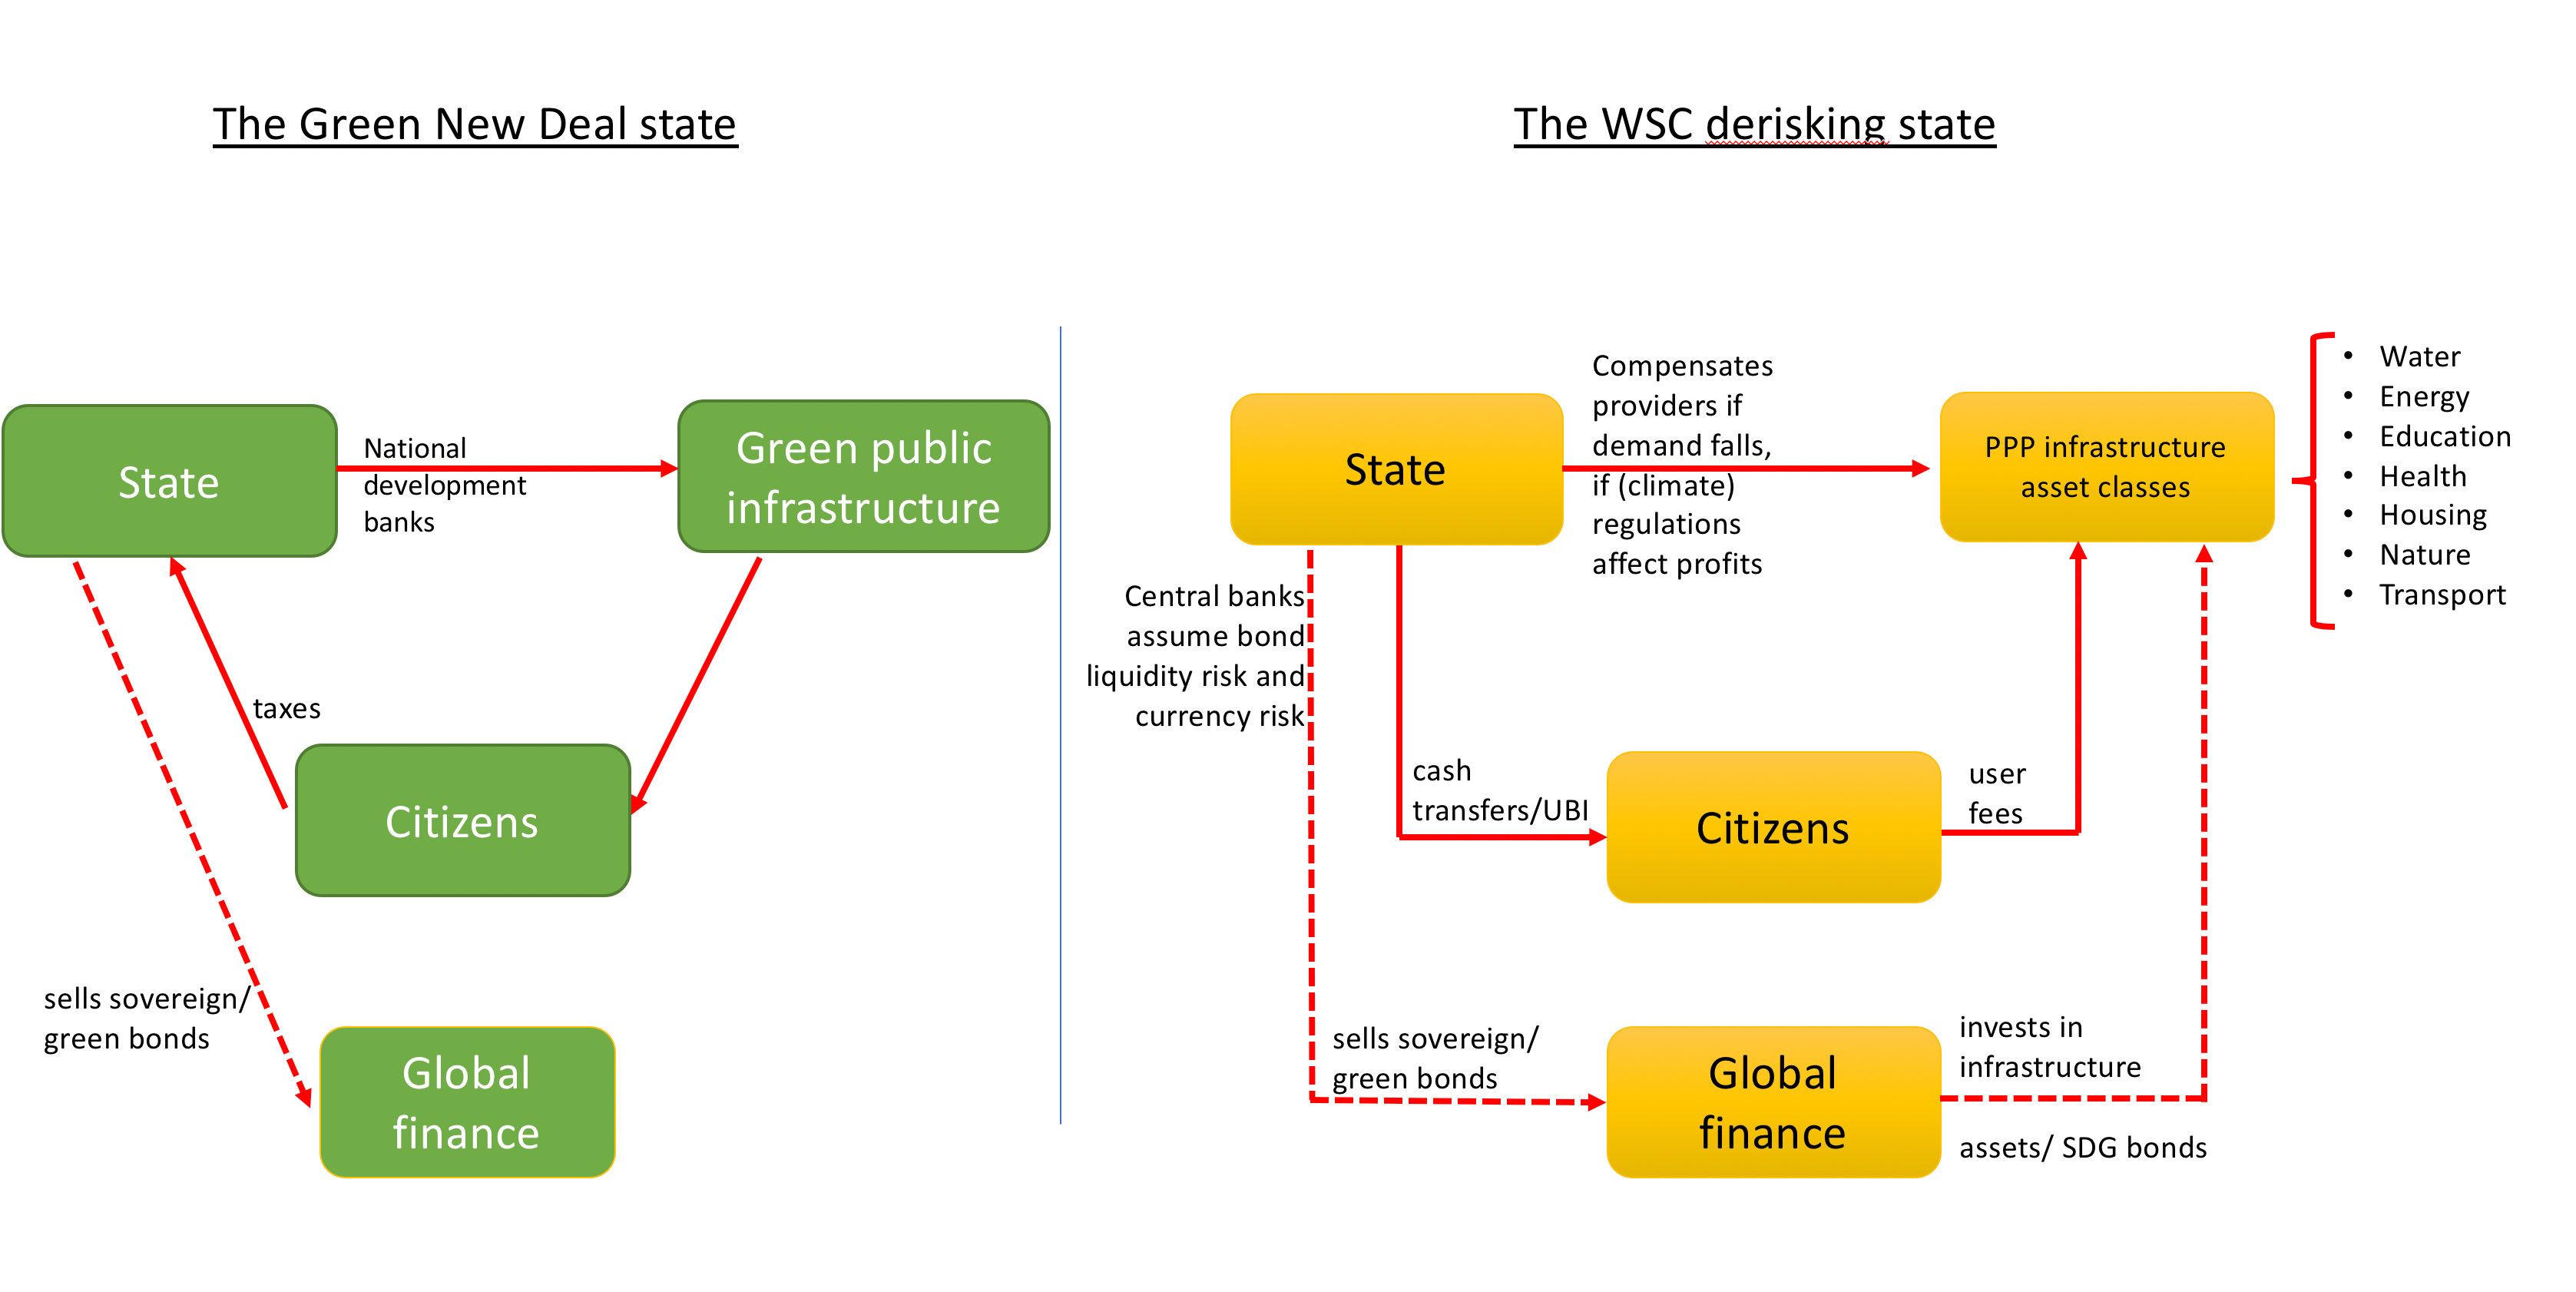
\includegraphics{fig/WSC_State.png}

In the derisking mode of governance, the state designs a menu of sector-specific policy
and financial derisking measures to encourage PPPs, accepts that this involves the
commodification of infrastructure via user-fees but puts in place cash
transfers/universal basic income schemes to mitigate the potential exclusion of the poor
from these services. That the derisking state does distributional politics through cash
transfers paradoxically accommodates calls for rethinking welfare politics as wage
labour becomes increasingly precarious.
Cash transfers enable the poor to access commodified public services,
and where these are not large enough, the state steps in to guarantee cash flows to investors.

Thus, development is not simply one-side defined by the political economy of capital,
but more specifically, by financial capital seeking to expand to new
areas, for which it colonises the infrastructure of the state. Financial capital no longer
just drags the poor into the embrace of the market, but also the state.

The derisking state can thus be understood as a project that seeks to extend the
infrastructural dependence of the state on finance -- and thus the infrastructural power
of the latter -- from its two traditional domains of monetary and fiscal policy to other
arenas of the government.

Derisking is not just about the transfers of risks to the state.
It is also about exercising infrastructural power to prevent
(regulatory) risks from materialising.

Derisking involves the central bank taking on its balance sheet bond liquidity and
currency market risks.

The legal battles to code capital into development asset
classes requires the state to take risks from the private sector onto its balance sheet, in
a clandestine reorienting of public resources that maintains the ideological commitment
to `fiscal responsibility'.

The WSC state assumes demand risk in user-fee based (social) infrastructure and
political risk that future governments might (re-)nationalize commodified
infrastructure or introduce tighter regulations, ranging from labour laws to climate
regulations that would affect profitability.

Uruguay's PPP law, passed by the
Mujica government in 2011, caps the total direct and contingent liabilities generated by
PPPs for the state to 7\% of the previous year's GDP, and fiscal transfers to private
operators to 0.5\% of previous year's GDP.

The fiscal costs of protecting investors from demand volatility will rise rapidly as
extreme climate events accelerate. Indeed, the climate crisis creates political and
demand risks that institutional investors need de-risking for.

The WSC protects investors against the political risks associated with green
developmental states. The green developmental state would prioritise the reorientation
of finance towards low-carbon activities. This requires a public taxonomy of green/dirty
assets that overcomes the shortcomings of private ESG ratings, and policies to penalize
dirty assets (through capital requirements or haircuts) 21 . Yet in the Wall Street
Consensus framework, such policies would classify as political risks, and require the
state to compensate their holders.

In its strategy to mutate climate risks into political and demand risks, private finance
may have found an important ally. Central banks conceptualize the immediate impact
of tighter climate rules regulation that increase the cost of funding or dramatically
change asset values as \emph{transition risks}.
The faster the low-carbon
transition, it is argued, the higher the potential that transition risks affect financial
stability, thus binding central banks in political trade-offs that privilege incremental
green regulatory regimes and accommodate greenwahing, however urgent the climate
crisis. Indeed, when central banks prioritize transition risks, they effectively rely on
private finance to drive the climate agenda, with their coordinating role focused on
subsidizing green assets, via so-called `green quantitative easing'.

In seeking to enlist central banks in the political coalitions against biting climate
regulation, the Wall Street Consensus constrains the green developmental states
directly, by making it liable for transition risks that can be framed as political and
demand risks, and indirectly, by reducing the public resources and central bank support
for Green New Deal programs that can effectively manage transition risks. The de-
risking state and the green developmental state can hardly co-exist, particularly within
market-based financial structures.

\textbf{Derisking market-based finance (formerly known as shadow banking)}

The turn to private finance as vehicle for sustainable development requires a change in
financial structures to accommodate the portfolio glut. It makes shadow banking,
understood as the production (via securitization) and financing (via wholesale funding
and derivative markets) of tradable securities, the desirable structure for financial
systems across the Global South. Indeed, the WSC consolidates
several global initiatives to restructure bank-based financial systems into market-based
finance or shadow banking,
where institutional investors can easily purchase local bonds (securities), including
infrastructure-backed securities, and finance as well as hedge their securities positions
via repos and derivative markets. Structural policies shift from developmental states'
concern with the productive structure, to the financial system.

The Financial Stability Board announced in 2015 that its new priority would be to transform
shadow banking into resilient market-based finance, which it defined as securities,
derivatives and repo markets.

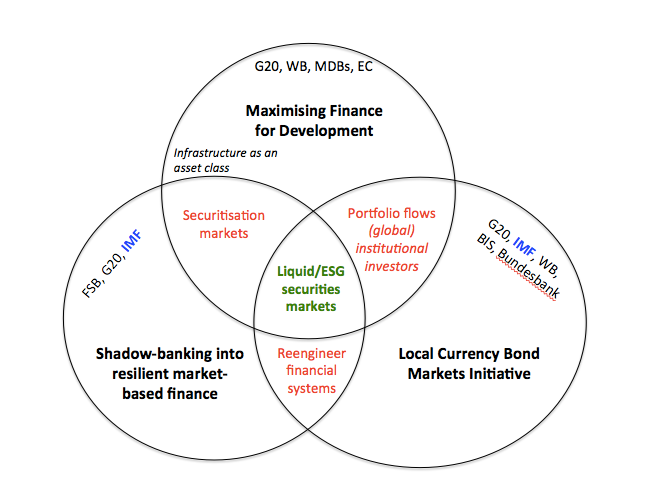
\includegraphics{fig/new_development_finance.png}

Figure: The turn to securities markets/market-based finance in international development

In sum, the organizational promoters of the Wall Street
Consensus championed in a multiplicity of global regulatory spaces the idea that
financial structure change is critical to attract the portfolio glut.

The
securitization of infrastructure loans would create both highly rated, low-return
tranches suitable for conservative pension funds/asset managers and lower-rated,
higher return tranches suitable for risk-driven investors. It would also accelerate lending
to infrastructure projects, constrained by Basel III rules for banks.

Since market-based finance is more systemically vulnerable than traditional bank-based
systems, the Wall Street Consensus assigns a triple de-risking role to central banks: in
bond markets and currency markets as market-makers of last resort,
and, forced by the inevitable consequences of green washing, as climate rescuers of last
resort, for assets left devalued by extreme climate events.
Some derisking
interventions, particularly in government bond markets, are at odds with the ideological
premises of central bank independence. Thus, the process of implicating central banks
in upholding the institutional basis of the derisking-centred accumulation regime is
incremental. It builds on crises such as the COVID19 pandemic to normalize new
derisking practices.

Greenwashing, like any
other regulatory arbitrage, eventually confronts its architects with the systemic
problems it feeds -- extreme climate events will devalue carbon-intensive assets and
greenwashed assets. The political logic of the Wall Street Consensus calls for central
banks to rescue the holders of last resort for carbon-intensive assets (Jahnke, 2019), to
risk-proof their portfolios, taking on its balance sheet the consequences of systemic
greenwashing.

`Development aid is dead, long-live private finance!'

\emph{Conclusion}

The Wall Street Consensus re-imagines international development interventions as
opportunities for global finance. In the new `development as derisking' paradigm,
institutional investors and asset managers are able to influence, if not altogether shape,
the terms on which poor countries join the global supply of `SDG' securities.
Multilateral development banks lead the efforts to design the ``de-risking''/subsidies
measures that seek to protect global investors from political risk or the demand risk
associated with privatized public services.

Equally important, this is a state-building project that puts in place the institutional
basis for a new regime of derisking as accumulation. The state comes under pressure
to institutionally codify risk-proofing arrangements, guaranteeing private financial
profits in the name of aligning sustainable projects with the preferred risk/return profile
of institutional investors. This includes adopting the US model of private pensions and
insurance to create local institutional investors. The tendency toward concentration in
the asset management sector (to exploit economies of scale and scope) may result in
Global North asset managers absorbing the funds of poor countries' institutional
investors and making allocative decisions on a global level.

In pushing for financial system change, development as derisking threatens to render
obsolete the old developmental banking model that put finance in the service of well-
designed industrial strategies. Development banks join the efforts of constructing and
derisking development asset classes. This is a political choice. Developmental banking
can arguably better serve a sustainability agenda because banks can easier include,
monitor and enforce safeguard policies in long-term relationships with customers. Most
countries with a successful experience of industrialisation relied on public development
banking as a critical pillar of industrial policies (Naqvi et al, 2018). Public development
banking allowed the developmental state to derisk via long-term loans to industrial
sectors identified as strategic by an industrial policy aimed at promoting the
international competitiveness of local firms.

This re-engineering of financial systems in the Global South, threatens the space for
alternative development strategies, and for a green developmental state. Government
capacity to design autonomous policies, in many poor countries severely eroded by
structural adjustment, will be further eroded by pressures to allocate scarce resources
to creating the conditions for private development finance.

\href{https://onlinelibrary.wiley.com/doi/abs/10.1111/dech.12645}{Daniela Gabor (2021) The Wall Street Consensus (Paywall)}
\href{pdf/Gabor_2021_Wall_Street_Consensus.pdf}{Draft (pdf)}

\hypertarget{imperialism-and-financialism}{%
\section{Imperialism and Financialism}\label{imperialism-and-financialism}}

\emph{Bichler \& Nitzan}

Over the past century, the nexus of imperialism and financialism has become a major axis
of Marxist theory and praxis. Many Marxists consider this nexus to be a cause of worldy
ills, but the historical role they ascribe to it has changed dramatically over time. The key
change concerns the nature and direction of surplus and liquidity flows. The first
incarnation of the nexus, articulated at the turn of the twentieth century, explained the
imperialist scramble for colonies to which finance capital could export its `excessive'
surplus. The next version posited a neo-imperial world of monopoly capitalism where the
core's surplus is absorbed domestically, sucked into a `black hole' of military spending
and financial intermediation. The third script postulated a World System where surplus is
imported from the dependent periphery into the financial core. And the most recent
edition explains the hollowing out of the U.S. core, a `red giant' that has already burned
much of its own productive fuel and is now trying to `financialize' the rest of the world in
order to use the system's external liquidity. This paper outlines this chameleon-like
transformation, assesses what is left of the nexus and asks whether it is worth keeping.

Our aim is to highlight the historical development of the
nexus of imperialism and financialism,
particularly the loose manner in which it has been altered --
to the point of meaning everything and nothing.

The paper comprises two parts. The first part examines the different schools. It
traces the transmutation of the nexus -- from its first articulation in the early twentieth
century, to the version developed by the Monopoly Capital school, to the arguments of
dependency and Word Systems analyses, to the thesis of hegemonic transition. The
second part offers an empirical exploration. Focusing specifically on the hegemonic
transition hypothesis, it identifies difficulties that arise when the theory meets the
evidence and assesses their significance for the century-old nexus.

\textbf{Empire and Finance}

The centralization of capital altered the political landscape. Instead of
the night-watchman government of the laissez-faire epoch, there emerged a strong, active
state.
The laissez-faire capitalists of the earlier era saw little reason to share their profits
with the state and therefore glorified the frugality of a small central administration and
minimal taxation. But the new state was no longer run by hands-off liberals. Instead, it was
dominated and manipulated by an aggressive oligarchy of `finance capital' -- a coalition of
large bankers, leading industrialists, war mongers and speculators who needed a strong
state that would crack down on domestic opposition and embark on foreign military
adventures.

The concentrated financialized economy, went the argument, requires pre-capitalist colonies
where surplus capital can be invested profitably; and the cabal of finance capital, now in
the political driver's seat, is able to push the state into an international imperialist
struggle to obtain those colonies.

At the time, this thesis was not only totally new and highly sophisticated; it also
fit closely with the unfolding of events. It gave an elegant explanation for the imperial
bellicosity of the late nineteenth century, and it neatly accounted for the circumstances
leading to the great imperial conflict of the first `World War'.

\textbf{Monopoly Capital}

In the brave new world of oligopolies, the emphasis on non-price competition
speeds up the pace of technical change and efficiency gains, making commodities cheaper
and cheaper to produce. But unlike in a competitive system, where market discipline
forces firms to pass on their lower costs to consumers, under the new circumstances, cost
reductions do not translate into falling prices. The prevalence of oligopolies creates a
built-in inflationary bias that, despite falling costs, makes prices move up and sometimes
sideways, but rarely if ever down.

This growing divergence between falling costs and rising prices increases the
income share of capitalists, and that increase reverses the underlying course of capitalism.
Marx believed that the combination of ever-growing mechanization and ruthless
competition creates a tendency of the rate of profit to fall. But the substitution of
monopoly capitalism for free competition inverts the trajectory. The new system
is ruled by an opposite `tendency of the surplus to rise'.

The early theorists of imperialism, although using a different vocabulary,
understood the gist of this transformation. And even though they did not provide a full
theory to explain it, they realized that the consequence of that transformation was to shift
the problem of capitalism from production to circulation (or in later Keynesian parlance,
from `aggregate supply' to `aggregate demand'). The new capitalism, they pointed out,
suffered not from insufficient surplus, but from too much surplus, and its key challenge
now was how to `offset' and `absorb' this ever-growing excess so that accumulation could
keep going instead of coming to a halt.

\textbf{Black Hole: The Role of Institutionalized Waste}

Until the early twentieth century, it seemed that the only way to offset the growing excess
was productive and external: the surplus of goods and capital had to be exported to and
productively invested in pre-capitalist colonies. But as it turned out, there was another
solution, one that the early theorists hadn't foreseen and that the analysts of Monopoly
Capital now emphasized. The surplus could also be disposed off unproductively and
internally: it could be wasted at home.

`Waste' denoted expenditures that are
necessary neither for producing the surplus nor for reproducing the population, and that
are, in that sense, totally unproductive and therefore wasteful. These expenditures absorb
existing surplus without creating any new surplus, and this double feature enables them to
mitigate without aggravating the tendency of the surplus to rise.

Use high military spending as a way to
secure the internal stability of U.S. capitalism.

The magnitude of military expenditures has no obvious ceiling: it
depends solely on the ability of the ruling class to justify the expenditures on the grounds
of national security. Similarly with the size of the financial sector: its magnitude expands
with the potentially limitless inflation of credit. This convenient expandability turns
military spending and financial intermediation into a giant `black hole'.

Spearheaded by U.S.-based multinationals and no longer hindered by inter-
capitalist wars, argued the theorists, the new order of monopoly capitalism has become
increasingly global and ever more integrated. And this global integration, they continued,
has come to depend on an international division of labour, free access to strategic raw
materials and political regimes that are ideologically open for business. However, these
conditions do not develop automatically and peacefully. They have to be actively
promoted and enforced.

Military spending comes to serve a dual role: together with the
financial sector and other forms of waste, it propels the accumulation of capital by black-
holing a large chunk of the economic surplus; and it helps secure a more sophisticated
and effective neo-imperial order that no longer needs colonial territories but is every bit
as expansionary, exploitative and violent as its crude imperial predecessor.

\textbf{Dependency}

The imperial powers relentlessly and systematically
undermined the socio-economic fabric of the periphery, making it totally dependent on
the core. And when decolonization finally started, the periphery found itself unable to
take off while the capitalist core prospered.
At that
point, there was no longer any need for core states to openly colonize and export capital
to the periphery. Using their disproportionate economic and state power, the former
imperialist countries were now able to hold the postcolonial periphery in a state of
debilitating economic monoculture, political submissiveness and cultural backwardness
-- and, wherever they could, to impose on it a system of unequal exchange.

This logic of dependent underdevelopment was first articulated during the
1950s and 1960s as an antidote to the liberal modernization thesis and its Rostowian
promise of an imminent takeoff.

Whereas earlier Marxist
theorists of imperialism accentuated the centrality of exploitation in production,
dependency and World-Systems analysts shifted the focus to trade and unequal
exchange. And while previous theories concentrated on the global class struggle,
dependency and World-Systems analyses spoke of a conflict between states and
geographical regions.

\textbf{Red Giant: An Empire Imploded}

`Financialization' is no longer a panacea for the
imperial power. On the contrary, it is a `sign of autumn', prime evidence of imperial
decline.

Finance (along with other
forms of waste) helps the imperial core absorb its rising surplus -- and in so doing
prevents stagnation and keeps accumulation going. But there is a price to pay. The
addiction to financial waste ends up consuming the very fuel that sustains the core's
imperial position: it hollows out the core's industrial sector, it undermines its productive
vitality, and, eventually, it limits its military capabilities. The financial sector itself
continues to expand absolutely and relatively, but this is the expansion of a `red giant' --
the final inflation of a star ready to implode.

The process leading to this implosion is emphasized by theories of hegemonic
transition.

The maturation of a hegemonic power -- be it Holland in the
seventeenth century, Britain in the nineteenth century or the United States presently --
coincides with the `over-accumulation' of capital.

This over-accumulation -- along with growing international rivalries,
challenges and conflicts -- triggers a system-wide financial expansion marked by soaring
capital flows, a rise in market speculation and a general inflation of debt and equity
values.
The financial expansion itself is led by the hegemonic state in an attempt to
arrest its own decline, but the reprieve it offers can only be temporary. Relying on finance
drains the core of its energy, causes productive investment to flow elsewhere and
eventually sets in motion the imminent process of hegemonic transition.

The United States benefited from being able to control,
manipulate and leverage this expansion for its own ends.
The growing severity of recent financial, economic and military crises suggests
that this ability has been greatly reduced and that U.S. hegemony is now coming to an end.

\textbf{End of Nexus?}

`Financialization' has not worked for the hegemonic power: despite the alleged
omnipotence of its Wall Street-Washington Complex, despite its control over key
international organizations, despite having imposed neoliberalism on the rest of the
world, and despite its seemingly limitless ability to borrow funds and suck in global
liquidity -- the bottom line is that the net profit share of U.S.-listed corporations has kept
falling and falling.

Of course, this isn't the first time that a monkey wrench has been thrown into the wheels
of the ever-changing nexus of imperialism and financialism. As we have seen, over the past
century the nexus has had to be repeatedly altered and transformed to match the
changing reality. Its first incarnation explained the imperialist scramble for colonies to
which finance capital could export its `excessive' surplus. The next version talked of a neo-
imperial world of monopoly capitalism where the core's surplus is absorbed domestically,
sucked into a `black hole' of military spending and financial intermediation. The third
script postulated a World System where surplus is imported from the dependent
periphery into the financial core. And the most recent edition explains the hollowing out
of the U.S. core, a `red giant' that has already burned much of its own productive fuel and
is now trying to `financialize' the rest of the world in order to use the system's external
liquidity.
Yet, here, too, the facts refuse to cooperate: contrary to the theory, they suggest
that the U.S. `Empire' has followed rather than led the global process of `financialization',
and that U.S. capitalists have consistently been less dependent on finance than their peers
elsewhere.

\href{http://bnarchives.yorku.ca/329/}{Bichler \& Nitzan (2012) Imperialism and Financialism}
\href{pdf/Bichler_Nitzan_2012_Imperialism_and_Financialism.pdf}{(pdf)}

\hypertarget{financial-system}{%
\chapter{Financial System}\label{financial-system}}

\emph{Ryan-Collins}

\textbf{Credit drives Housing Prices}

One of the most remarkable, but
neglected, macroeconomic shifts in the past 50 years has been the
transformation of banking systems in advanced economies from their
textbook role of lending to non-­financial firms for working capital
and investment to becoming real estate lenders ( Jordà et al.~2017).
Mortgage lending in advanced economies increased on average from
40 percent of GDP in the mid-­1990s to almost 70 percent by the finan-
cial crisis of 2007--­2008, whilst the stock of business loans rose by
little more than 5 percent ( Jordà et al.~2017). During the same period,
average real house prices followed a path similar to that taken by
mortgage credit, doubling in value, suggesting credit was the primary
driver of rising prices.

\href{https://onlinelibrary.wi\%20ley.com/doi/10.1111/ajes.12387}{Ryan-Collins (2021) Private Landed Property and Finance: A Checkered History}
\href{pdf/Ryan-Collins_2021_Private_Landed_Property_and_Finance.pdf}{(pdf)}

\hypertarget{asset-manager-capitalism}{%
\section{Asset Manager Capitalism}\label{asset-manager-capitalism}}

\begin{quote}
Asset manager capitalism is a structure of power. It is interwoven with policy. It has expanded at the same time as central bank asset purchases (QE) have become the key tool of macro-policy. It is expanding the frontiers of financialization into every area of life. Asset managers need yield. They get yield by financializing everything from real estate to natural capital. And this is capitalism. It is interwoven with social structure, inequality and class.
\end{quote}

\emph{Braun}

The political economy literature explains
financialization in the United States as the result of policymakers -- for reasons specific
to the American political economy between the late 1960s and early 1980s -- turning to
financial markets to solve problems of governability and profitability. My argument,
although compatible with this conjunctural explanation, instead emphasizes the
macroeconomic -- and historically recurring -- process of wealth accumulation as an
underlying, structural cause.

The puzzle that arises from this
argument: the strange non-death of the rentier in an era of financial capital abundance.
Keynes predicted that once the resource the financial sector controls became abundant,
the ``cumulative oppressive power of the capitalist to exploit the scarcity-value of capital''
would decline. Recent economic history has borne out the first part of Keynes' prediction,
but not the second: Finance capital has become abundant, but the rentier has returned
to ``rude health''

As per Piketty, the best measure of this
health is the gap between the rate of return on capital (r) and the rate of economic
growth (g). Subsequent work has shown this gap to have proven
remarkably resilient in recent decades.

My central proposition is that whereas capital scarcity increases the exit-based structural
power of finance, capital abundance strengthens the ownership- and control-based
structural power of finance.

The asset management sector comprises, first and
foremost, mutual funds and exchange-traded funds, as well as the less regulated and
more leveraged institutions, namely hedge funds, private equity funds, and venture
capital funds. 8 Although the distinction tends to get blurry in practice, there is a
fundamental difference between institutional investors that are asset \emph{owners}, and asset
\emph{managers} that are pure intermediaries in the business of managing other people's money
for a fee-

The asset management sector has seen exceptional growth over the
past half century. What is more, since the global financial crisis of 2008 most global
banks have greatly expanded their asset management arms, as have many insurers. On
the list of the world's top-10 asset managers, the ``Big-Three'' asset managers
(BlackRock, Vanguard, and State Street Global Advisors) are closely followed by the
asset management arms of Goldman Sachs, Allianz, and the like.

The assets of investment funds started to rise steeply in the 1980s and especially the
1990s, and today stand at twice the level of bank assets loans.
The growth of institutional capital pools in general, and the concentration of the asset
management sector in particular, have fundamentally reshaped financial markets and the
structure of financial asset ownership.

share ownership concentration,
believed to be an anachronism belonging to the finance capital era, made a comeback
through the backdoor of the retirement-asset fueled lengthening of the investment chain.
As a result of
this ``Great Re-concentration'', the United States is no longer the dispersed ownership
society that scholars across disciplines and across generations -- from Berle and Means,
to Jensen and Meckling, to Hall and Soskice -- took for granted.

Large, voice-affording stakes and full diversification
ceased to be mutually exclusive; while liquidity -- and thus the exit option -- had
evaporated. This combination makes asset manager capitalism historically unique, and
the implications for the structural power of wealth owners and their financial
intermediaries are by no means straightforward.

In their quest for scale, large asset
managers have essentially relinquished the option to exit individual investments.
This is a consequence, first, of the size of
their stakes in individual companies -- which even in a liquid market cannot be sold
without causing a major drop in the share price. Second, the loss of exit is a feature of
the index-tracking investment strategies pursued by the majority of funds offered by the
Big-Three asset managers. The existing theoretical framework would predict the
structural power of large asset managers to be weakened by this loss.

The loss of the exit option is compensated, however, by the increase in \emph{voice}. One source
of asset manager voice is the brute voting power that comes with large shareholdings.
Their voting power makes the large index-tracking asset managers key allies for hedge
funds, which routinely seek the support of the Big Three for their activist campaigns.

The second source of asset manager voice is \emph{diversification}. The Big Three have promoted
the narrative that their fully diversified (``universal'') shareholdings make them the
quintessential long-term shareholders, whose interests are aligned with environmental,
social, and governance (ESG) objectives.

Whether asset managers actually wield their structural power, and in whose interest,
remains an open question.
If the logic of universal ownership
is compelling in theory, in practice it is counteracted by a host of ``agency problems'',
ranging from the cost of exercising voice to the cost of alienating the corporate managers
who control the allocation of retirement plan assets to competing asset managers.

Asset managers' dominant role in capital
markets affords them infrastructural power vis-a-vis fiscal and monetary authorities.
Hiring BlackRock to support their market operations has become routine
for central banks around the world.

Asset managers'
overriding preference is for welfare state policies that increase private household savings
and, crucially, for macroeconomic policies that sustain high asset prices.
This
shift in financial-sector preferences has far-reaching implications for the political economy
of macroeconomic policy.

\href{pdf/Braun_2021_Asset_Mamager_Capitalism.pdf}{Braun (2021) Asset Manager Capitalism (pdf)}

\emph{Tooze}

We live in a remarkable world. As of July 20 2021, three asset managers, BlackRock, Vanguard Group and State Street Corp.~collectively owned about 22\% of the average S\&P 500 company, according to data compiled by Bloomberg, up from 13.5\% in 2008.

On Benjamin Braun:

INVESTMENT is about wealth preservation NOT productivity enhancement!

Financial capital has become abundant in the global economy. The logic of supply and demand would suggest that wealth owners and their financial intermediaries should see their structural power decline. Paradoxically, the ultimate gauge of rentier power -- the gap between the rate of return on capital (r) and the rate of economic growth (g) -- has proven remarkably resilient since the 1980s. Why did this gap not shrink? The guiding hypothesis of this project is that the power of wealth owners is partly a function of the organization of finance. The project studies the rise of different types of asset managers -- firms that pool and manage ``other people's money'' -- and their impact on the economic and political determinants of the rate of return on capital.

Asset manager capitalism differs from early 20th-century ``finance capital'' because unlike the banks studied by Hilferding, today's asset management giants combine control with diversification.

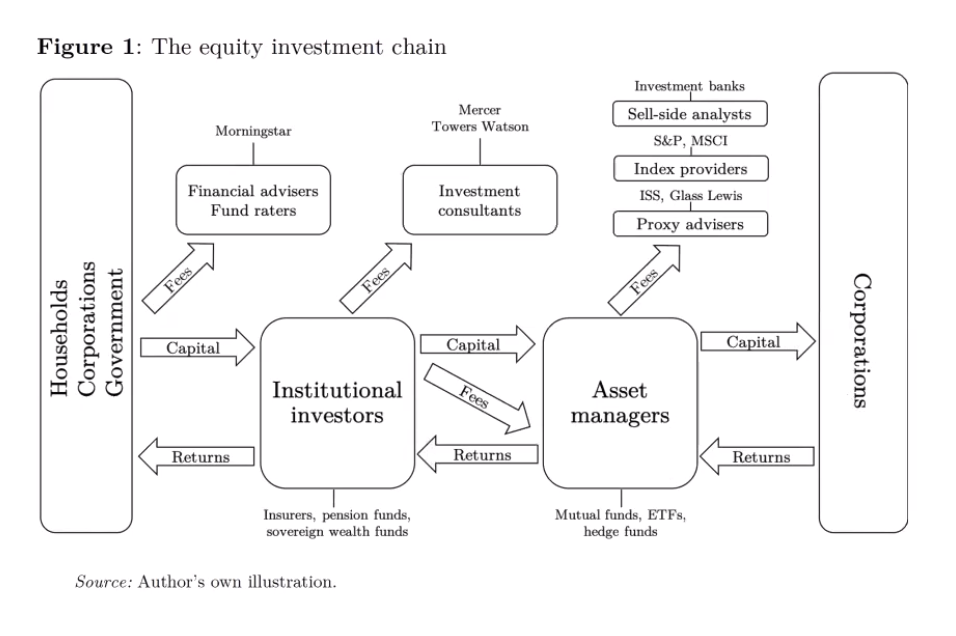
\includegraphics{fig/asset_manager_capitalism.png}

The key point to recognize is how asset managers earn their money. It isn't through the returns of the corporations they invest in, but through the fees paid to them by institutional investors who aggregate the funds of households, corporations, governments etc.
Those fees, of course, will ultimately only roll in if the asset managers earn good returns. But, if you stripped this down, the households could ultimately own the assets themselves. Adding the intermediation, advice, expertise, reduction of complexity etc etc is the key to the entire business.

Asset managers are mediated owners. They are mediated also as a result of the sheer size of their portfolios. They are radically diversified, owning slices of practically every corporation worth anything. But their bulk means that their ability to exit stock is limited. They are simply too big.

Like a robber baron, BlackRock has achieved a high concentration of ownership. Unlike a robber baron it has a huge diversification of what it owns and a limited interest in any particular bit of its portfolio. This somewhat paradoxical state of being into everything and unable to get out, gives rise to the idea that asset managers are what is called ``universal owners''.

Not only do institutional investors own a majority of the public equity of the world, but through that ownership, their success as investors is dependent on the performance of the economy at large. Large owners who own a representative ``slice'' of the economy are more dependent on general macroeconomic performance than on the performance of any one stock or portfolio.

What BlackRock wants is exorbitant. It wants the public balance sheet to step in backstop any risks that asset managers might be running (in making serious ESG investments.)

And because BlackRock is a huge universal owner, when it asks for a public backstop it means the public balance sheet of the world - no kidding!

It is almost as though someone at BlackRock has been reading the \emph{Communist Manifesto} and is asking themselves: Where is that ``committee for managing the common affairs of the whole bourgeoisie'' that we were promised? And no, a 1990s-style ad hoc combo of Greenspan-Summers-Rubin won't do the trick. Universal owner → universal public backstop please!

The fundamental different political economy produced when government conceives its role as being essentially to derisk investment by gigantic private asset managers.

Focusing on 2008 encapsulates the shift from a bank-centered financial model to the rise of asset management. In 2008-9, banks were discredited by the crisis and literally began to cannibalize themselves to survive.

\begin{quote}
Asset manager capitalism is a structure of power. It is interwoven with policy. It has expanded at the same time as central bank asset purchases (QE) have become the key tool of macro-policy. It is expanding the frontiers of financialization into every area of life. Asset managers need yield. They get yield by financializing everything from real estate to natural capital. And this is capitalism. It is interwoven with social structure, inequality and class.
\end{quote}

\href{https://adamtooze.substack.com/p/chartbook-82-the-rise-of-asset-manager}{Tooze (2022) The Rise of Asset manager Capitalism}

\emph{Braun}

\emph{Asset Manager Capitalism} is a historically distinct corporate governance regime. Whereas
the control-based dominance of finance capital during the early 20 th century was
characterized by credit-debt relationships between banks and corporations, today asset
managers' equity holdings dominate; and whereas the shareholder capitalism of the late
20 th century was characterized by impatient investors wielding the threat of exit, the
power of asset managers in corporate governance is based on their large and illiquid, yet
fully diversified shareholdings. Recent evidence suggests that the structural power
wielded by asset managers determines corporate governance outcomes on environmental
and social issues, influences product market competition, and shifts the macroeconomic
policy preferences of the financial sector.

\href{https://osf.io/preprints/socarxiv/4uesc}{Braun (2022) From Exit to Control}
\href{pdf/Braun_2022_From_exit_to_control.pdf}{(pdf)}

\hypertarget{financialization}{%
\chapter{Financialization}\label{financialization}}

\emph{Braun}

Financialization in the United States has been
explained as the result of the exhaustion on the
Fordist growth model. Competition in interna-
tional trade, de-industrialization, and disinfla-
tionary policies all put pressure on political
actors to liberalize finance so that newly cre-
ated credit could substitute for stagnating wage
income and sustain aggregated demand. 11
However, as historians Fernand Braudel and
Giovanni Arrighi have argued, financialization
has been a recurring feature of capitalist devel-
opment. It tends to be driven by a slowdown of
accumulation that makes reinvesting profits in
immobile productive capital relatively less
attractive to capitalists, who instead seek
returns from liquid financial claims.

\href{pdf/Braun_2021_Fueling_Financialization_Funded_Pensions.pdf}{Braun (2021) Fueling Financialization: The Economic Consequences of Funded Pensions (pdf)}

\hypertarget{washington-consensus}{%
\section{Washington Consensus}\label{washington-consensus}}

\emph{Copley}

\textbf{Financialization Was a Response to Capitalism's Failings}

Popular critiques of financial deregulation often blame the City of London's excessive political influence. But financialization wasn't imposed on capitalism by elite plotting --- it was a political response to its inherent crisis tendencies.

Financialization refers to the growing size and importance of financial markets in global capitalism since the 1970s. Credit bubbles have inflated, colossal banking institutions have swallowed up smaller ones, and complex financial instruments have proliferated. Many industrial corporations have also become financialized, earning increasing revenues from financial ventures and reinvesting them in short-term schemes to boost share prices. Everyday life, too, has been transfigured. We are increasingly pressured to approach our lives like balance sheets, making prudent investments, managing risk, and acquiring financial assets (chiefly housing) to insulate ourselves against economic uncertainty.

This process of expanding financial logics has been accompanied by another development, referred to as ``secular stagnation'' or the ``long downturn.'' Global capitalism's dynamism has waned following the end of the post--World War II economic boom. Since the 1970s, profitability, investment, and GDP growth have remained relatively stagnant. What paltry growth the world economy has enjoyed in recent years has depended on continuous interventions by central banks, which have channeled vast quantities of money into financial markets in an attempt to stimulate a boom.

The era of financialization has thus witnessed both financial expansion and economic stagnation. Ours is a world in which stories of record-breaking stock market rallies share the news cycle with gloomy growth projections and spectacular images of revolts by the poor and policed.

How did we arrive at this point? It's important to understand that financialization was not, in fact, a spontaneous market development --- rather, it was deeply political. This phenomenon was engineered by advanced capitalist states through policies of financial liberalization during the 1970s and 1980s, and then it was exported around the world under the banner of the \textbf{Washington Consensus}.

Britain lies at the heart of this story. Margaret Thatcher's radical liberalization of the UK's banking sector was instrumental in forging a global financial order in which the City of London is a crucial hub. Indeed, some of the worst practices revealed by the 2008 crash were conducted by the London branches of global banks. As Peter Gowan observed, the City became for Wall Street ``something akin to what Guantánamo Bay would become for Washington: the place where you could do abroad what you could not do back home.''

The key UK policies that propelled financialization were not primarily driven by financial lobbying or neoliberal doctrine, nor were they part of a larger political blueprint. Instead, these liberalizations were messy, ad hoc attempts to address the political quandaries churned up by the ``stagflation'' crisis of the 1970s and early 1980s --- itself generated by capitalism's inherent crisis tendencies.

These liberalizations were not designed to cater to City elites. Indeed, they endangered the guaranteed profits of many London bankers, exposing them to competition from foreign conglomerates that dwarfed them in scale and sophistication. These policies often found greater support from the Confederation of British Industry than from financial lobbies. Neither were they straightforward enactments of neoliberal dogma. First, they began in 1971, before the so-called ``neoliberal revolution.'' Second, they were geared to address more mundane governing problems. Far from a cunning blueprint, these policies were ``a leap in the dark,'' as Thatcher's financial secretary (and future chancellor) Nigel Lawson called them.

The British liberalizations that propelled financialization were desperate, pragmatic attempts to navigate the contradictory imperatives of global capitalism and domestic politics in a moment of deep crisis.

It is unclear whether our conquest of the state, to which so much energy has recently been devoted, could put the financial genie back in the bottle --- at least not without generating equally objectionable side effects. Financialization was the result of politicians struggling with the real contradictions of governing capitalism. Socialists today, were they to win office, would face these same contradictions. Chief among them is that the capitalist state's very capacity to act depends upon profitable labor exploitation within its territory. Policymakers are not dominated by conniving financiers but by this impersonal compulsion to achieve profitability, which emanates from capitalism's marketized social relations.

Financial liberalizations represented one strategy to negotiate this ugly reality. If a leftist government reversed these liberalizations, it would need to offer an alternative plan to marry popular legitimacy with the lucrative exploitation of its citizenry. For this reason, no matter who signs the executive orders, the state cannot simply ``build a new society just as well as a new railway,'' as Marx once remarked. It cannot legislate for a just world when injustice sustains it. This is the confounding strategic terrain that confronts us as we seek to wrestle with capitalism's out-of-control financial logics.

\href{https://jacobinmag.com/2021/12/financialization-city-london-margaret-thatcher-england}{Copley (2021) Financialization Was a Response to Capitalism's Failings}

\hypertarget{macro-finance}{%
\chapter{Macro Finance}\label{macro-finance}}

\emph{Cochrane Abstract}

Macro-finance addresses the link between asset prices and economic fluctuations.
Many models reflect the same rough idea: the market's ability to bear risk is greater
in good times, and less in bad times. Models achieve this similar result by quite dif-
ferent mechanisms. I contrast their strengths and weaknesses. I highlight directions
for future research, including additional facts to be matched, and limitations of the
models that should prod future theoretical work. I describe how macro-finance mod-
els can fundamentally alter macroeconomics, by putting time-varying risk premiums
and risk-bearing capacity at the center of recessions rather than variation in the
interest rate and intertemporal substitution.

\emph{Cochrane Memo}

Asset prices and returns are correlated with business cycles. Stocks rise in good times,
and fall in bad times. Real and nominal interest rates rise and fall with the business cycle.
Stock returns and bond yields also help to forecast macroeconomic events such as GDP
growth and inflation. 1
Stocks have a substantially higher average return than bonds. Typical estimates put the equity
premium between 4\% and 8\%. Even 4\% is puzzling. Why do people not try to hold more stocks,
given the power of compound returns to increase wealth dramatically over long horizons?

The answer is, of course, that stocks are risky. But people accept many risks in life. In
lotteries and at casinos they even seek out risks. The answer must be that stocks have a spe-
cial kind of risk, that stock values fall at particularly inconvenient times or in particularly
inconvenient states of nature.

So, just what are the bad times or bad states of nature, in which investors are particularly
anxious that their stocks do not fall? Well, something about recessions is an obvious candi-
date. Losing money in the stock market is especially fearsome if that event tends to happen
just as you lose your job, your business is losing money, you may lose your house, and so on.
But what is the feared event exactly? How do we measure that event? And what does
this fear that stocks might fall in recessions tell us about the macroeconomics of recessions?
These questions are what macro-finance is all about.

Why are people so afraid of stocks when they do not seem that afraid
of other events?

In sum, we face two main questions. First, the equity premium question: What is there
about recessions, or some other measure of economic bad times, that makes people particu-
larly afraid that stocks will fall during those bad times---and so people require a large up-
front premium to bear that risk? Second, the predictability question: What is there
about recessions, or some other measure of economic bad times, that makes that premium
rise---that makes people, in bad times, even more afraid of taking the same risk going
forward?

The
consumption-based model works well at a qualitative level, as does the story that people
are afraid of recessions, and become more risk averse during recessions. The challenge is to
find concrete, quantitative, and theoretically explicit measures of fearful outcomes and of
risk aversion, that quantitatively account for asset pricing facts.

**Macro-finance vs Macro-economics*

Though called ``macro-finance'' this literature still stands quite apart from macroeco-
nomics. Macroeconomics by and large does not use, for understanding recession-related
quantity and goods-price dynamics, the preferences or market structures that macro-
finance uses to understand recession-related asset pricing dynamics. Macroeconomics by
and large ignores first-order effects of uncertainty, focusing on ``the'' short term interest
rate and the consequent allocation of consumption over time.

The central lesson of macro-finance denies this approximation: Business cycle-related
asset price fluctuations are all about variation in risk premiums.

In recessions, both consumption and investment fall, and so output and the labor to pro-
duce it fall. Most theories of business cycles therefore start with two questions: First, why
does consumption fall? Second, why does a rise in desired saving not produce a rise in in-
vestment? These questions have been the heart of macroeconomics since Keynes.

Macro-finance suggests that recessions, such as fall 2008, are not times at which
people became thrifty, saving more to provide a better tomorrow, and they are certainly
not times of high real interest rates. Macro-finance suggests that people consumed and in-
vested less because they were scared to death---because of risk, risk aversion, high risk pre-
miums, precautionary savings, not because of sudden thriftiness and a wrong level of the
overnight federal funds rate.

Corporate investment has very little relationship with real interest rates, despite the prevalence of this channel in macroeconomic models.

The key to falling investment, then, is a mismatch between the riskiness of real corpor-
ate investment projects, and the higher risk aversion of savers.

This is not the only path to greater unity between macroeconomics and macro-finance,
of course. It allows us to merge the relatively frictionless preference- or market-structure
based models (habits, recursive utility, idiosyncratic risk, rare disasters) that generate time-
varying risk aversion with the standard general-equilibrium aggregative models that per-
vade macroeconomics. But the behavioral view, as outlined above, might suggest instead a
reverse causality by which behavioral misperceptions in stock markets spill over to macro-
economics, or it might suggest a pervasive behavioral misperception behind both macro
and finance. And merging macroeconomics with asset pricing is the rallying cry of the insti-
tutional finance/frictions research agenda, which aims to put pervasive credit constraints,
balance sheet imbalances, agency frictions, and so forth at the heart of macroeconomics as
well as of asset pricing.

\href{https://academic.oup.com/rof/article/21/3/945/3060346}{Cochrane (2017) Macro-Finance}
\href{pdf/Cochrane_2017_Macro-Finance.pdf}{(pdf)}

\hypertarget{postwar-macrofinancial-regime}{%
\section{Postwar Macrofinancial Regime}\label{postwar-macrofinancial-regime}}

\emph{Braun}

The macro-financial regime of the postwar
period was characterized by substantial financial
repression. Strict financial regulation and
controls on international capital mobility subor-
dinated private finance to the interests of the
non-financial and the public sectors. To the
extent funded pension systems existed, they
were ``characterized by a close proximity
between the state and pension funds.''

\href{pdf/Braun_2021_Fueling_Financialization_Funded_Pensions.pdf}{Braun (2021) Fueling Financialization: The Economic Consequences of Funded Pensions (pdf\\
)}

\hypertarget{money-1}{%
\chapter{Money}\label{money-1}}

\begin{quote}
Money is the alienated essence of man's labour and life; and this alien essence dominates him as he worships it. (Karl Marx)
\end{quote}

\hypertarget{regulation}{%
\chapter{Regulation}\label{regulation}}

\hypertarget{complexity-theory-and-financial-regulation}{%
\section{Complexity Theory and Financial Regulation}\label{complexity-theory-and-financial-regulation}}

\begin{itemize}
\tightlist
\item
  Battiston Abstract*
\end{itemize}

Traditional economic theory could not explain, much less predict, the near collapse of the financial system and its long-lasting effects on the global economy. Since the 2008 crisis, there has been increasing interest in using ideas from complexity theory to make sense of economic and financial markets. Concepts, such as tipping points, networks, contagion, feedback, and resilience have entered the financial and regulatory lexicon, but actual use of complexity models and results remains at an early stage. Recent insights and techniques offer potential for better monitoring and management of highly interconnected economic and financial systems and, thus, may help anticipate and manage future crises.

\emph{Battiston Memo}

Recent research on contagion in
financial networks has shown that network
topology and positions of banks matter; the
global financial network may collapse even
when individual banks appear safe.

Information asymmetry within a net-
work---e.g.~where a bank does not know
about troubled assets of other banks --- can
be problematic. The banking network typically displays a core-periphery structure,
with a core consisting of a relatively small
number of large, densely interconnected
banks that are not very diverse in terms of
business and risk models. This implies that
core banks' defaults tend to be highly correlated.
That, in turn, can generate a collective moral hazard problem (i.e., players
take on more risk, because others will bear
the costs in case of default), as banks recognize
that they are likely to be supported by
the authorities in situations of distress, the
likelihood amplifies their incentives to herd
in the first place.

Publicly available bank information does not allow reliable estimation of systemic risk. The
estimate would improve greatly if banks
publicly reported the number of connections with other banks, even without
disclosing their identity.

Too-central-to-fail may be even more important than
too-big-to-fail.

Recent experiments studying behavior
of a group of individuals in the laboratory
show that economic systems may deviate
significantly from rational efficient equilibrium at both individual and aggregate
levels (14). This generic feature of positive
feedback systems leads to persistent deviations
of prices from equilibrium and emergence of speculation-driven bubbles and
crashes, strongly amplified by coordination
on trend-following and herding behavior.
There is strong empirical evidence of
monetary and fiscal policies and financial
regulation designed to weaken positive feed-
back are successful in stabilizing experimental
macroeconomic systems when properly
calibrated. Complexity theory provides
mathematical understanding of these effects.

\href{https://www.science.org/doi/10.1126/science.aad0299}{Battiston (2021)}
\href{pdf/Battiston_2021_Complexity_Theory_and_Financial_Regulation.pdf}{(pdf)}

\hypertarget{institutionalizing-esg}{%
\section{Institutionalizing ESG}\label{institutionalizing-esg}}

\emph{Beslik}

Suddenly, millions of influential, wealthy and beyond imagination privileged people in the financial and corporate sectors around the world realised that ``Oh, this is no good anymore. We need to deploy `non-financial' metrics to understand the value of companies we invest in and run, from financial point-of-view.''

Just like that? Well, maybe not. But I think one of the most relevant answers to how this has happened does not come from sudden and enormous pressure from clients (they usually don't even know what they are buying on ESG since they lack information) or from a prophetic moment in the morning-mirror for millions of people in the financial and corporate sector asking themselves how they can save the world.

If you try to track down some of the key drivers you can see the traces going back to 2008 when people working in the financial sector and their decisions driven by the only God (money) shook the entire world -- and billions of people around the world paid a price, some with their life.

Politicians reacted too late and too lame, and most of the losses were paid for collectively, i.e.~tax money. For too long, self-regulation and voluntary, business driven responsibility was championed as most efficient symbiosis for the benefit of all, or very few.

After 2008, politicians might have learned the lesson that self-regulation and voluntary responsibility by the financial and corporate sectors means different things to different actors.

In the climate negotiations in Copenhagen and in Paris (two among the hundreds of conferences on climate change and consequences related to that, that I have participated in over last 20 years) the financial industry was largely absent. It was not there, or just there to observe. Despite its size and influence, despite its power, the financial sector does not have any climate targets discussed and agreed upon on a global level -- neither from the COP negotiations, nor via any other transnational agreements.

That's changing now. \emph{It's the regulation in the EU and by now partly in the US that is the key driver behind ESG growth}, both in terms of interest and in terms of assets.

Yes, those grey politicians in the different parts of the world are by all means changing the word of investments by posing rules, sometimes in the need of improvement, yet rules that institutionalise ESG. Not as an add-on, as self-regulated nice-to-have things you can market to clients. But as a law.

This, if anything, is monumental, and in the years to come regulation, nothing else, forced by reality, will completely reshape the social contract between the financial industry and societies at large.

It is both needed and necessary if ESG is meant to make real changes on the ground.

\href{https://esgonasunday.substack.com/p/week-19-esg-on-a-sunday-turns-1-}{Beslik}

\hypertarget{central-banks-1}{%
\chapter{Central Banks}\label{central-banks-1}}

\begin{quote}
Never ever say the words `central banks control the money supply'.
\end{quote}

\begin{quote}
Central banking is more akin to sailing than driving. Whilst it might be tempting to imagine them steering the economy with a reliable accelerator and brake, they are far more at the mercy of the elements. They can tack and trim with a greater or lesser degree of skill, but in the end they can't change the wind.
\end{quote}

In managing our economy with disembedded measures of wealth,
the world's central bankers are effectively agents of the sustainability crisis. They may not
wish to be unsustainable by personal inclination, but they certainly are by professional
obligation because of how they are duty-bound to act.
An entirely foreseeable response to the climate emergency is that people in wealthier
countries may choose to pare back their consumption of non-essentials. Certainly, not
everyone has the luxury to do this, but the obvious solution of ``buying less stuff'' has become
an articulated idea in wealthy countries. ``Flight shaming'' and ``consumption shaming'' are new
memes. Articles in multiple UK newspapers have challenged readers to see if they can go a
year without buying any new clothes, contravening the media's normal practice of generally
trying to coax the economy along. (It buoys the advertising revenue).
Such behaviours would amount to a direct hit on GDP in developed countries, where personal
consumption can represent two-thirds of the total. Critically, any such reduction in
consumption will likely show up as a deflationary decline in economic activity that the world's
central banks are on hair-trigger alert to prevent. The large and powerful financial
bureaucracy stands ready to provide immediate stimulus to any perceived flagging of
measured economic activity.
Hence, the arrangement most populations in the world currently live under is that should they
collectively choose to buy less, more money will be printed until they have changed their
mind. Effectively, our exhausted ecosystem is gasping for a lull in measured economic activity
that our financial authorities are pledged to never let happen.

\href{pdf/Austin_2021_Pigou_\%20and_the_dropped_stitch_of_economics_RWER95.pdf}{Duncan Austin: Pigou and the dropped stitch of economics RWER95 (pdf)}

\hypertarget{macroprudential}{%
\section{Macroprudential}\label{macroprudential}}

Macroprudential policies are financial policies aimed at ensuring the stability of the financial system as a whole to prevent substantial disruptions in credit and other vital financial services necessary for stable economic growth. The stability of the financial system is at greater risk when financial vulnerabilities are high, such as when institutions and investors have high leverage and are overly reliant on uninsured short-term funding, and interconnections are complex and opaque. High vulnerabilities increase the likelihood that a firm's failure or other negative shock would cause distress at other financial institutions because of direct exposures and through fire sales, contagion, or other negative externalities arising from the initial shock. Macroprudential policies aim to reduce the financial system's sensitivity to shocks by limiting the buildup of financial vulnerabilities.

One example of a macroprudential policy is the higher capital charge applied to Global Systemically Important Banks (G-SIBs), banks that pose more risk to the system. The G-SIB capital surcharge is based on five types of characteristics viewed to increase a bank's systemic risk: size, complexity, interconnectedness, lack of substitutes, and cross-jurisdictional activity. Higher capital charges reduce the likelihood that a G-SIB would fail because they will have thicker capital cushions to absorb losses.

A \href{https://www.brookings.edu/research/understanding-the-effects-of-the-u-s-stress-tests/}{recent paper} looks at how the macro scenarios and assumptions about dividends and share repurchases in the stress tests work to reduce procyclicality of capital requirements.

Macroprudential tools can be structural or cyclical. Structural policies are implemented to build lender or borrower resilience to adverse events at any point in the business cycle. For example, the additional capital charges for G-SIBs are a structural tool. In other countries, limits on loan-to-value ratios (LTVs) or debt service--to--income ratios (DSTIs) for mortgage borrowers are examples of structural tools that have been applied to borrowers. These limits can be macroprudential when they are intended to not only protect an individual borrower from too much debt, but to protect home values in neighborhoods from falling sharply because many borrowers have trouble making their payments at the same time. The Hong Kong Monetary Authority, for example, sets the LTV ratios for borrowers based on the value of the property. Bank borrowers for properties with high values could get mortgages with LTV ratios ranging from 40 percent to 60 percent, while they could get mortgages with higher LTV ratios, up to 70 percent, for properties with low values.

Cyclical policies are aimed at increasing resilience in anticipation of an economic downturn to lessen the reduction in the supply of credit once the downturn materializes. The countercyclical capital buffer (CCyB) is an example of a cyclical policy. The CCyB works by requiring banks to increase their capital cushions during an economic expansion when systemic risks are rising, and then release them in an economic downturn to absorb losses. Reducing the capital constraint by releasing the buffer when the economy slows helps to insure against deleveraging, which if not counteracted could deepen the downturn by restricting credit.

Historically, macroprudential policies have been used more often in emerging market economies than in advanced economies. But since the global financial crisis, both advanced economies and emerging market economies have been using macroprudential measures more frequently.

\href{https://www.brookings.edu/blog/up-front/2020/02/11/what-are-macroprudential-tools/}{Brookings}

\hypertarget{central-bank-independence-1}{%
\section{Central Bank Independence}\label{central-bank-independence-1}}

\emph{Haldane Memo}

The widespread adoption of central bank independence was born out of the economic situation of the 1970s. The Great Inflation had seen high and persistent inflation across the world and economists turned their attention to the role that monetary policy played in this phenomenon. The time-consistency theory of Kydland and Prescott (1977), Nordhaus (1975) and Barro and Gordon (1983) provided an elegant answer to what might be going on. Governments had a natural tendency to over-inflate their economies, especially around election time, generating an ``inflation bias''. To curb this inflation bias, some institutional means was needed to constrain government's policy hand. Rogoff (1985) developed a model which provided such an institutional fix. Monetary policy decisions were to be delegated to a ``conservative'', inflation-minded, central bank acting independently from government. In this way, central bank independence could prevent, at source, a return to the Great Inflation of the 1970s.

The macro-economic benefits, in theory, did not end there. Provided inflation expectations were well-anchored and central banks were not too inflation-averse -- ``inflation nutters'' in the language of Mervyn King -- monetary policy could be effective in stabilising output in the economy too. In other words, central bank independence was a potential twin-win, reducing inflation biases at no cost in increased output variability -- a free lunch.

Empirical evidence followed to test these hypotheses. During the 1980s and 1990s, a number of papers established a statistically significant link between the level and variability of inflation and the degree of central bank independence across a range of countries. These cross-country correlations strongly suggested central independence was an important contributor to reduced inflation bias (Chart 3) and that it wasn't associated with increased variability in output (Chart 4). The free lunch in theory was there in practice too. And this evidence, in turn, helped spur moves towards central bank independence in the latter-part of the 20th century.

Interestingly, a look at more recent time periods suggests these observed associations have vanished since the start of the 21st century (Charts 5-7). What explains this disappearing correlation? Some have used it to question whether the earlier link between independence and low inflation was no more than a statistical mirage. It could be argued that the fall in inflation over this earlier period was instead the result of the benign macro-economic environment of the Great Moderation. In other words, better inflation outcomes in the late 20th century might have reflected good luck rather than good central bank management.

The time-consistency problem familiar from monetary policy has a clear read-across to the world of financial stability. Governments have an incentive to run their financial systems, as well as their economies, hot in the interests of growth and electoral advantage. This generates a tendency to loosen regulation too far during credit booms, increasing the risk of future bouts of financial instability. In other words, there is a potential problem of ``instability bias'' in regulatory policies, to accompany the ``inflation bias'' in monetary policies.

In fact, I would argue this time-consistency problem is potentially greater in the financial stability sphere than for monetary policy, for two reasons. Credit cycles tend to be longer in duration, and larger in amplitude, than typical business cycles. This means wishful thinking and policy myopia (``this time is different'') are more likely to arise in credit booms than during typical business cycle upswings, exaggerating the time-consistency problem of financial stability policies.
The costs of financial instabilities and crises also tend to larger than the costs of inflationary surges. This means the temptation to act in a time-inconsistent fashion -- talking tough ex-ante, but acting weak ex-post -- also tends to be greater. That can encourage risk-taking and amplify financial cycles and crises -- a doom loop. The Global Financial Crisis, a long-duration credit boom that prompted massive government support ex-post, was a good example of these acute financial stability time-consistency problems in practice.

Given the practical success of independence, it is important to guard it for the future. And there are potential threats here. Central banks around the world have expanded their balance sheets massively over the past decade, and particularly over the past year. While this is not monetary financing, it has blurred the line between the monetary and fiscal realms and, among some people, raised questions of independence. The test will come if and when inflation begins to rise and central banks need to tighten policy to meet their mandate, independently of the prevailing fiscal stance. At that point, the strength and effectiveness of the legal and institutional frameworks surrounding independence will be crucial in ensuring we continue to benefit from the twin-wins that have been a feature of the last few decades.

\href{https://bankplassen.norges-bank.no/2021/04/16/central-bank-independence-a-practitioners-perspective/\#more-1994}{Haldane}

\hypertarget{market-neutrality}{%
\subsection{Market Neutrality}\label{market-neutrality}}

The principle of market neutrality posits that corporate bonds purchased under the ECB's €270bn corporate sector purchase programme should be made in a `neutral' way: they should reflect the overall eligible market to ensure they do not distort the relative pricing of securities. Given the concentration of carbon-intensive industries in the corporate bond universe, this has resulted in a carbon-biased portfolio. This is problematic as it exposes the ECB to climate-related risks. And yet central bankers have so far been reluctant to question market neutrality for fear of losing their independence.

\href{https://www.omfif.org/2021/02/ecb-market-neutrality-crumbling/}{Kyriakopoulou}

\emph{Klooster Abstract}

Monetary policy operations in corporate security markets confront central
banks with choices that are traditionally perceived to be the prerogative of
governments. This article investigates how central bankers legitimise
corporate security purchases through a comparative study of the
European Central Bank (ECB) and the Swiss National Bank (SNB). As we
show, central bankers downplay the novelty of corporate security
purchases by relying on familiar pre-crisis justifications of Central Bank
Independence. Citing an ideal of `market neutrality', central banks
present corporate security purchases as pursuing a narrow objective of
price stability and obfuscate their distributive consequences. In this way,
central bankers depoliticise corporate security purchases: they reduce
the potential for choice, collective agency, and deliberation concerning
both the pursuit of corporate security purchases and the choices made
in implementing these policies. We also describe the undesirable
democratic, social and environmental dimensions of these practices,
which we propose to address through enhanced democratic
accountability.

\emph{Klooster Memo}

The past decades saw central banks acquire considerable independence from democratic institutions
(McNamara 2002, Singleton 2010). Governments justified their decision to delegate monetary policy
by relying on a narrow conception of monetary policy. This conception focuses on the setting of short
term interest rates to achieve a long-term objective of stable price levels. A crucial element in the
justification of central bank independence is the idea that monetary policy is an apolitical, technical
area of policymaking (Marcussen 2009). The loss of democratic control that results from the creation
of an independent central bank was also thought to be minimal, because distributive choices would
remain with elected governments, who both decided on the central bank mandate and retained the
use of fiscal instruments to achieve their distributive objectives. In this way, governments depoliticised
monetary policy in the sense of reducing the potential for choice, collective agency, and deliberation
around the use of monetary policy

The Global Financial Crisis (GFC) led central bankers to move far beyond the narrow task assigned
to them under the traditional justification of Central Bank Independence (CBI)
To rescue a global financial system on the brink of collapse, central bankers assumed new roles as lenders and market makers of last resort.

Central bankers, meanwhile, are openly concerned that the use of unconventional tools threatens
their independence.
When independent regulatory agencies extend their power, political authorities often seek to regain
control.
Central bankers, accordingly, try to counteract repoliticisation and these efforts
shape their policies.

To investigate the simultaneously occurring processes of politicisation and depoliticisation
we investigate how central bankers relate to the political dimensions of their
new unconventional policies.

QE increases wealth inequalities.

Central bankers depoliticise their security purchases by subsuming
them under the pre-crisis justification of CBI.

Central bankers present themselves as pursuing price stability,
while in reality engaging in these purchases for reasons that are entirely unrelated to price stability.

\emph{`Market Neutrality'}

Rather than acknowledging and
managing the market impact of their policies, central bankers pursue `market neutrality', e.g.~they
seek to minimise the impact of their purchases on the relative prices of financial assets.

Central bankers keep decisions on new monetary instruments in the domain of their
expert judgment, and thereby outside the domain of democratic politics.

As a consequence of their effort to make corporate security purchases market neutral,
these programmes are insufficiently sensitive to environmental and societal concerns.

Depoliticisation of monetary policy: First, independent
central banks treat monetary policy as having a narrow objective, which can be achieved with a
clearly-defined toolbox and, second, central bankers treat distributive consequences as insignificant
and sanctioned by the central bank's mandate.

\href{https://www.tandfonline.com/doi/epub/10.1080/13563467.2019.1657077?needAccess=true}{Klooster (2021) The Myth of Market Neutrality}
\href{pdf/Klooster_2021_Myth_of_Market_Neutrality.pdf}{(pdf)}

The new exogenous money is exogenous transition shocks in the climate change debate.
Fortunately, Bank of England cannot hide behind that rock because of their new climate mandate.

Remember, Mark Carney's `tragedy of the horizons' speech identified two main risks of climate crisis:
- physical risks (climate events)
- transition risks - from green policies to accelerate transition to low-carbon

Now, central banks are confronted with an unpleasant conundrum that reveals the deeply political nature of their operations:
greening monetary policy (collateral, unconventional bond purchases) means endogenous transition risks

So, in a have your cake and eat it moment, there is a growing tendency in central bank communities to pretend that all transition risks come from the fiscal side (carbon pricing)

It wouldn't be surprising to find the exogenous transition shocks approach in the ECB's monetary policy strategy review, despite \citet{Lagarde}
and other's recognition that central banks cannot longer hide behind the `market neutrality' argument.

\href{https://twitter.com/DanielaGabor/status/1384837864412917765}{Gabor (Twitter)}

\hypertarget{financial-stability-1}{%
\section{Financial Stability}\label{financial-stability-1}}

\hypertarget{climate-risk-1}{%
\subsection{Climate Risk}\label{climate-risk-1}}

\textbf{BIS Recommendations}

This report provides an overview of conceptual issues related to climate-related financial risk
measurement and methodologies, as well as practical implementation by banks and supervisors.

The report contains five key findings:
First, climate-related financial risks have unique features, necessitating granular and
forward-looking measurement methodologies.

Second, to date, measurement of climate-related financial risks by banks and supervisors
has centred on mapping near-term transition risk drivers into counterparty and portfolio exposures.

Third, banks and supervisors have predominantly focused on assessing credit risk, as they
advance in applying methods to translate climate-related exposures into categories of financial risk.

Fourth, while banks and supervisors remain at an early stage of translating climate-related
risks into robustly quantifiable financial risk, work continues to gather pace

Fifth, key areas for future analytical exploration relate to measurement gaps in data and
risk classification methods, as well as methodologies suitable for assessing long-term climate
phenomena not always of a standard nature.

\href{https://www.bis.org/bcbs/publ/d518.htm}{BIS (2021) Climate Risk}
\href{pdf/BIS_2021_Climate_Risk.pdf}{(pdf)}

\textbf{Institutional Dynamics}

\emph{Baer Abstract}

This article studies how institutional dynamics might affect the implementation of climate-
related financial policies. First, we propose a three-dimensional framework to distinguish: i)
motives for policy implementation (prudential or promotional); ii) policy instruments
(informational, incentive or coercive); and iii) implementing authorities (political or
delegated). Second, we use this framework to show how sustainable financial interventions in
certain jurisdictions - most notably, Europe - rely solely on informational policies to achieve
both promotional and prudential objectives. Policymakers in other jurisdictions - e.g., China -
also implement incentive or coercive financial policies to achieve promotional objectives.
Third, we identify two main institutional explanations for this European `promotional gap': i)
limited control of political authorities on financial dynamics; and ii) strong powers and
independence of delegated authorities. This governance configuration leads to an institutional
deadlock in which only measures fitting with both political and delegated authorities'
objectives can be implemented. Finally, we discuss the scenarios that might originate from the
current institutional setting. We identify three possible evolutionary paths: i) a drift towards a
green financial technocracy; ii) a re-politicization of delegated authorities; iii) a move towards
fiscal-monetary coordination.

\emph{Baer Memo}

In 2017, the EU Commissioner Valdis Dombrovskis expressed his support to the idea of
introducing a `green supporting factor' in bank capital requirements to incentivize lending to
sustainable activities (Dombrovskis, 2017). The following year, the European Commission
included the idea of `incorporating sustainability in prudential requirements' in its sustainable
finance action plan (EC, 2018). This position was generally greeted with skepticism by most
central bankers and financial supervisors (see, among others: Dankert et al., 2018; Elderson,
2018; Rehn, 2018). It was emphasized that the aim of prudential rules is to mitigate financial
risk, not to steer private credit in any particular direction. \emph{According to central bankers and
financial supervisors, capital requirements should not discriminate between green and dirty
financial assets, unless clear evidence of risk differentials is available.}

This recent clash between public institutions raises deeper questions. For what purposes should
banking and financial regulation be used? And who should decide what the admissible
purposes are?

EU Banking regulation cannot be employed as a
policy tool to actively reallocate private financial resources towards sustainable investments.

In several emerging economies banking and financial regulation is instead
actively used to promote specific productive sectors.
Financial risk is still monitored, but stronger
weight is given to development (e.g., green) objectives.

The current status quo is unsustainable due to environmental constraints. At some
point, someone will need to introduce stronger promotional policies to steer credit towards
sustainable sectors. Given the distribution of responsibilities, missions, and powers crystallized
within the current institutional framework, these promotional efforts should be led by the
political authorities, leaving delegated authorities with a supporting role.

\href{pdf/Baer_2021_Institutional_Climate_Policy_Dynamics.pdf}{Baer (2021) Climate-related financial policies (pdf)}

\hypertarget{climate-change-impact-on-central-banks}{%
\subsubsection{Climate Change Impact on Central Banks}\label{climate-change-impact-on-central-banks}}

\emph{Batten Abstract}

This paper examines the channels via which climate change and policies to mitigate it could affect a
central bank's ability to meet its monetary and financial stability objectives. We argue that two types of
risks are particularly relevant for central banks. First, a weather-related natural disaster could trigger
financial and macroeconomic instability if it severely damages the balance sheets of households,
corporates, banks, and insurers (\emph{physical risks}). Second, a sudden, unexpected tightening of carbon
emission policies could lead to a disorderly re-pricing of carbon-intensive assets and a negative supply
shock (\emph{transition risks}). Climate-related disclosure could facilitate an orderly transition to a low-carbon
economy if it helps a wide range of investors better assess their financial risk exposures.

\emph{Batten Memo}

Our analysis builds on Bank of England (2015) and
Carney (2015) which have examined the impact of climate change on the insurance industry, but
broadens the scope of the analysis. Specifically, our paper examines the impact of climate
change and the changes in the composition of energy supply associated with the transition to a
low-carbon economy on the financial system and the macroeconomy, and thus goes beyond the
analysis of the European Systemic Risk Board (2016) that considered the potential impact of the
transition to a low-carbon economy on financial stability. While climate change is expected to
have more adverse macroeconomic impacts on some developing countries, the focus of this
paper is mainly on the impact of climate change from the perspective of central banks in
advanced economies.

Without CCS, 35\% of known global oil, 52\% of gas and 88\% of coal reserves will
be `unburnable' before 2050 in order to achieve the 2oC target.

The carbon price (which could take a form of a carbon tax or determined via a carbon
emission trading scheme) would need to be about €35-60/tCO 2 for CCS coal-fired power plants
to compete against coal-fired plants with unabated emissions, and €90-105/tCO 2 for CCS-gas
fired plants to compete against gas-fired plants with unabated emissions.

Financial sector activities can influence physical risks through a number of channels. First, the
decision of financial institutions to fund activities that are intensive in CO 2 emissions can
contribute to increasing the climate-related physical risks, albeit indirectly; and conversely, their
financing of technologies that help reduce CO 2 emissions can contribute to a reduction of
climate-related physical risks. This is a problem of externalities, as the financial institutions that
fund these activities do not necessarily suffer the losses and gains resulting from changes in
climate-related physical risks, most of which may occur in the future, and hence may not
internalise these losses and gains when making the funding decisions. The standard ways of
addressing such externalities include appropriate use of taxes and subsidies, and legislation that
directly targets the specific externalities.

By contrast, prudential regulations are fairly blunt instruments for dealing with climate-related
externalities. For example, capital requirements for banks and insurers are designed to mitigate
prudential risks, and hence adapting these to reflect externalities could undermine their primary
purpose, or could give rise to undesirable effects.
On the one hand, relaxing regulations just to
encourage particular types of lending, for example by reducing risk weights that are used in
calculating the regulatory capital ratios below their prudentially sound levels, could jeopardise
the safety and soundness of financial institutions. 12 On the other hand, tightening regulations on
financial exposures to carbon-intensive firms could also have the unintended effect of increasing
the cost of finance for those borrowers, thus reducing their ability to invest in emission-reducing
technologies (e.g.~CCS and renewables), unless exclusions can be applied to financing
specifically earmarked for such investments. Thus, targeted policy measures are more likely to
be effective in achieving climate-related objectives than adapting prudential regulations.

both the size of the financial losses arising from the occurrence of a given hazard and
the allocation of those losses are influenced by the \emph{ex ante} decisions of the financial sector.
For
example, the amount of insurance and credit available for financing the construction of
buildings in flood-prone areas will determine the size of the eventual financial losses arising
from the materialisation of such risks, as well as the allocation of these losses. The market
outcome can be expected to be efficient as long as all contracting parties are fully aware of the
risks and can price them efficiently, but various market imperfections could result in mispricing
of risks. For example, the price of insurance could be driven up if asymmetric information leads
to adverse selection problems, in which only those parties that are inherently higher risk than
average choose to buy insurance. 13 Moreover, uncertainty about the wider repercussions of
extreme weather events implies that certain risks -- such as the likelihood that they trigger riots
that could cause further damage -- are inherently hard to model.

The materialisation of climate-related physical risks -- e.g.~via natural disasters that are
influenced by climate change -- can potentially result in large financial losses, some of which are
borne by insurers while others are uninsured.

\emph{Batten Conclusion}

This paper has examined the impact of climate change on the monetary policy and financial
stability objectives of central banks. We have identified four main ways in which climate
change and policies on carbon emissions could affect central banks' objectives.
First, a weather-related natural disaster could trigger financial instability and a macroeconomic
downturn if it causes severe damage to the balance sheets of households, corporates, banks and
insurers (physical risks). The economic impact of a given natural disaster is likely to be less
severe if the relevant risks are priced in financial contracts ex ante, and the financial system has
distributed them efficiently, e.g.~via insurance and reinsurance. Ex post, a central bank will need
to react appropriately to a disaster to meet its monetary and financial stability objectives by
gauging the impact on the output gap, inflationary pressure and the financial system -- for
example, by adjusting monetary policy and supplying liquidity to the financial system if needed.
Second, gradual warming could also affect an economy's potential growth rate. However, more
reliable quantitative estimates based on detailed sector-level impact analysis would be needed
before central banks can incorporate this effect in their monetary policy analysis.
Third, a sudden, unexpected tightening of carbon emission policies could lead to a disorderly re-
pricing of carbon-intensive assets and generate a negative supply shock (transition risks). This
has a potential for generating significant balance sheet losses and financial instability. An
orderly transition to a low-carbon economy is possible, and is likely to be facilitated by
transparent and predictable policies on carbon emissions that encourage an early re-direction of
private investment towards low-carbon technologies. Climate-related disclosure by industries
could encourage this re-direction if it enables a wide range of investors to better assess their
financial risk exposures. Such disclosure is likely to be more effective if it is both forward-
looking and simple to understand -- for example, how a given change in carbon price will affect
the value of the firm. Such disclosure could potentially also help inform the central banks'
assessment of financial stability risks arising from the transition to a low-carbon economy, for
example via a stress test.
Finally, both the changes in weather patterns and the increased reliance on bioenergy could
increase the volatility of food and energy prices, and hence the volatility of headline inflation
rates. This could make it more challenging for central banks to gauge underlying inflationary
pressures and maintain inflation close to the target.

\href{https://www.bankofengland.co.uk/working-paper/2016/lets-talk-about-the-weather-the-impact-of-climate-change-on-central-banks}{Batten (2016) Impact of climate change on central banks}

\hypertarget{sustainable-regulation}{%
\subsubsection{Sustainable Regulation}\label{sustainable-regulation}}

WWF today launches a new framework -- Sustainable Financial Regulations and Central Bank Activities (SUSREG) -- to support central banks, financial regulators and supervisors in enhancing the financial sector's stability and resilience to climate-related and broader environmental and social risks, while enabling the mobilisation of capital for the transition to a low-carbon, resilient and sustainable economy.

Developed as part of WWF's Greening Financial Regulation Initiative, the SUSREG framework will be used to assess the extent to which climate-related, environmental and social issues are being integrated in key aspects of financial regulations, supervisory expectations and monetary policy in 40 countries, covering most members and observers of the Basel Committee on Banking Supervision (BCBS).

\href{https://wwf.panda.org/?1834441/Sustainable-Financial-Regulations-SUSREG}{WWF}

\hypertarget{feds-dollar-empire}{%
\section{FED's Dollar Empire}\label{feds-dollar-empire}}

The return the Federal Reserve makes on its portfolio managing the dollar empire. In 2015, the Fed remitted \$97 billion in profits to the US Treasury; compare that to the \$88 billion made by the most profitable company in the world, Saudi Aramco.

That money is treated like tax money---the Treasury reduces the federal debt by that amount.
The Treasury reduces the federal debt by that amount, diminishing the quantity of safe assets in the world.

\href{https://phenomenalworld.org/analysis/reconstruction-finance}{Johnson}

\hypertarget{eu-macroprudential}{%
\section{EU Macroprudential}\label{eu-macroprudential}}

\emph{Stellinga Abstract}

The 2007--09 financial crisis appeared to demonstrate the need for a strong, supranational EU macro‐prudential policy framework to prevent similar future disasters. The implemented framework, however, is neither. It is highly complex, involving many constraints on the use of macro‐prudential instruments. It is also one of the principal areas of national discretion in EU banking regulation. To explain this, I build on the `financial trilemma' thesis which holds that there are inherent tensions between pursuing financial stability, financial integration and national financial policies. Supranationalizing macro‐prudential policy proved difficult due to a lack of consensus on how to measure systemic risks and because of the distributional consequences involved. This increased the tension between stability and integration, as national macro‐prudential policies could constrain cross‐border finance and they could be misused for competitiveness considerations. Key policy actors disagreed on which goals to prioritize, with bargaining leading to a convoluted policy framework.

\emph{Stellinga Memo}

MPP targets systemic risks by enabling supervisors to tighten requirements during booms, to loosen them when risks recede, and to impose tougher rules on systemically important financial institutions.

Given the devastating consequences of the crisis and EU policy‐makers' embrace of macro‐prudential ideas, a strong MPP framework seemed a likely post‐crisis outcome. Especially in light of the EU's push for regulatory harmonization -- both the single rulebook and the shift (in the Eurozone) towards supranational supervision by the European Central Bank (ECB) reduced national discretion in micro‐prudential regulation -- we would have expected a harmonized framework to emerge for macro‐prudential policy.

The implemented framework did not meet these expectations.
Although supervisors gained new macro‐prudential instruments, their use has been constrained by procedural requirements and limits to their stringency and scope, with macro‐prudential instruments focusing on capital requirements and leaving other segments of banking regulation and the non‐banking sector largely untouched.

Systemic risk is an elusive concept with an important national dimension, rendering a one‐size‐fits‐all approach counterproductive.

The MPP framework that developed between 2009 and 13 was the result of key actors' inability to agree on how to balance national discretion, stability and integration.

With no consensus on how to measure systemic risks, supranational macro‐prudential norms implied a one‐size‐fits‐none approach. As systemic risks change over time, relying on a fixed set of indicators could well mean preparing for yesterday's war.

\href{https://onlinelibrary.wiley.com/doi/full/10.1111/jcms.13195}{Stellinga}

\hypertarget{finance-influence}{%
\section{Finance Influence}\label{finance-influence}}

\emph{Braun Abstract}

The pre-crisis rise and post-crisis resilience of European repo and securitization markets represent political victories for the interests of large banks. To explain when and how finance wins, the literature emphasizes lobbying capacity (instrumental power) and the financial sector's central position in the economy (structural power). Increasingly, however, finance also enjoys infrastructural power, which stems from entanglements between specific financial markets and public-sector actors, such as treasuries and central banks, which govern by transacting in those markets. To demonstrate the analytical value of this perspective, the article traces how the European Central Bank (ECB), motivated by monetary policy considerations, has shaped post-crisis financial policymaking in the EU. It shows that the ECB has played a key part in fending off a financial transaction tax on repos and in shoring up and rebuilding the securitization market. With market-based forms of state agency on the rise, infrastructural entanglement and power shed new light on the politics of finance.

\emph{Braun Memo}

Following the global financial crisis, the European Commission proposed taxing repos and
reining in securitization, in an effort to tackle the two financial markets at the heart of
European shadow banking. Several years and policy battles later, repos are exempt from a
defanged financial transaction tax proposal, while reviving securitization is a top EU policy
priority. Why did financial-sector interests prevail? Proposing a new theoretical approach to
the politics of finance, this article focuses on the power relations at the hybrid intersection of
private banking and public central banking.

Much has been written about the politics leading up to and protecting central bank
independence, which both stems from and entrenches
unequal power between capital and labour in a low-salience, technocratic policy area. In
contrast, the literature has less to say about how, once central bank independence is
established, power operates at the intersection of public monetary authority and private financial
markets.

The marketization of financial intermediation is a key aspect of financialization.
The rise of what has variously been labelled `shadow banking', `securitized banking'
or `market-based banking' has been a boon to the financial sector.
Fee-based income, regulatory arbitrage, bigger balance sheets and higher leverage ratios
have boosted profits and remuneration.
Despite being seen as the chief culprit of the global financial crisis, market-
based banking has shown remarkable resilience since 2008.
In Europe, following a brief period of stigmatization, it is at the heart of
`Capital Markets Union', the European Commission's attempt to build a more market-based
financial system.
This surprising outcome indicates substantial political support for financial-sector interests.

The political economy literature emphasizes two forms of political power wielded by the
financial sector: instrumental power, exercised through lobbying, and structural power,
which derives from the financial sector's privileged position in financialized economies.

This literature has
yielded important results, but its treatment of the state and of finance as two separate
spheres, and of state agency as purely regulatory, is problematic. It is at odds with the crucial
insight of a discipline-spanning body of research that maintains that, at the centre of the
financial system, state and market actors form a hybrid public--private partnership, or a
franchise system.

Whereas the regulatory view conceptualizes state--finance interactions
as `regulation and governance through rule making and rule enforcement', this article,
drawing on the hybridity view, maintains that state agency is often
market-based---state actors appear not just as regulators of but also as participants in financial
markets.

This article advances a simple theoretical argument: when state actors transact in finan-
cial markets for governance purposes they create infrastructural entanglements, which con-
stitute a distinct source of financial-sector power. In the case at hand, repo and
securitization markets---the two main pillars of market-based banking---provide the infra-
structure through which the European Central Bank (ECB) implements its monetary policy.
This entanglement makes central bankers, who seek to maximize their economic steering
capacity, dependent on bankers, giving the latter infrastructural power. This has
distributional consequences: financial institutions benefit from their infrastructural role in the
monetary system, including through interest payments on central bank reserves---which
come at a fiscal cost to taxpayers --- and through preferential treatment in the political process.

The political power that accrues to private financial actors as a result of
state actors seeking to govern through financial markets.

Explaining the ECB's support for repo and securitization markets by the central
bank's dependence on these financial infrastructures, the article adds an important piece to
the puzzle of how finance wins, while at the same time highlighting policymaking as a facet
of central banking that, at a time of heightened concerns about central bank independence
and legitimacy.

The political economy literature has shed light on the delegation of power to cen-
tral bank technocrats, but has failed to elucidate the politics of how, once empowered,
central bankers act on the economy.

This became particularly problematic when, in the context
of financial liberalization in the 1980s, central bank agency became more market-based.
Specifically, central banks shifted from `direct' to `indirect' monetary policy instruments---
the triad of reserve requirements, standing facilities and open market operations.
As part of the latter, central banks, including the ECB, adopted financial
practices from the private sector, notably mark-to-market techniques, margin calls and hair-
cuts.
The ECB took the marketization of monetary policy to new
heights when, in 2005, it outsourced the decision over the collateral eligibility of euro-area
sovereign bonds to private credit rating agencies.

ECB is different from other EU gov-
ernance bodies. It is not only a central bank that holds and exerts administrative authority---
`setting, interpreting and applying statutory rules'---but also a central bank that trades in
financial claims with other, private-sector banks.

The central bank's control over macroeconomic conditions depends on financial transactions
into which private actors enter at their own discretion, creating infrastructural entanglements with
those financial markets that serve as the conduits for monetary policy.

Traditionally, European banks have
engaged in relationship-based lending financed by customer deposits. While banks continue
to play a central role in European credit intermediation, the hallmark of the new business
model has been the marketization of both sides of banks' balance sheets.
On the asset side, banks securitize loans into asset-backed securities that are sold
to investors. On the liability side, banks complement deposit financing by borrowing in the
secured money market, where securities (including securitized loans) serve as collateral. This
business model of market-based banking is part of the broader shadow banking system that
includes non-bank financial institutions, such as money market mutual funds and asset managers.

From a political economy perspective, market-based banking, and shadow banking more
broadly, matter for three main reasons: systemic risk, corporate finance and inequality.
The 2008 systemic financial crisis was caused by losses on securitized loans on the asset side and
a freeze of short-term money market funding on the liability side of banks' balance sheets
The buffer function associated
with relationship-based banking is diminished with market-based banking,
under which borrowing conditions for firms and households depend much more
directly on developments in global capital markets.
The marketization of financial intermediation has been a key contributor to
the growth in inequality in OECD countries.

The financial sector's high levels of unity and organization often
bring favourable political outcomes.

The dependence of the state on private and the resulting structural power of
business in general, and of finance in particular.
The distinguishing feature of structural power is that it achieves political
forbearance without the need for business to organise and act in concert.

The central bank and the treasury---routinely enter transactions with
private-sector counterparties, buying and selling financial
claims for public policy purposes. This leads to the main theoretical argument of the present
article: those parts of the financial system that serve as conduits for such market-based
economic governance enjoy infrastructural power. Closely related to structural power in that it
rests on the financial sector's centrality for economic performance, infrastructural power
nevertheless constitutes a distinct sub-type derived from direct entanglement at the level of
policy instruments rather than the indirect dependence at the level of ultimate policy goals.

According to the structural power approach policymakers placate business interests
for fear that not doing so would harm economic growth.
In contrast, infrastructural power operates via policymakers' expectation that harming
particular markets would blunt their own policy instruments and thus
diminish their control over the economy.

The European Commission and the ECB may be working towards complementary and
compatible goals, but they do so by different methods: the Commission governs by issuing
directives and regulations, the ECB by issuing liabilities and purchasing securities.

The ECB's support for repo and securitization markets is underpinned by
a rational expectations-based macroeconomic paradigm
that implies a positive net effect of deep and liquid financial markets on economic
performance and governability.

Central bankers protect finance in order to bolster their own
institutional position and independence.

\emph{Repo}

While there was still considerable instrument diversity in the 1990s, by 1997 most EMU
central banks had converged on reverse repurchase transactions as their primary reserve-
providing instrument, thus paving the way for them to become the
standard instrument for all open market operations of the Eurosystem (that is, the ECB and
the national central banks). A sale and repurchase agreement, or repo, consists of an
exchange of cash for securities between two parties. The cash borrower (`repo seller') agrees
to repurchase the securities from the cash lender (`repo buyer') at a specified date in the
future. Interest is paid by the cash borrower in the form of a mark-up on the repurchase
price, the repo rate. Repo markets are at the heart of the global shadow banking system. In
addition to the interbank segment, repo markets also connect banks in search of short-term
funding and non-bank institutions seeking safe and liquid, money-like assets.
Following the crisis, repo markets came under scrutiny for their effects on
pro-cyclicality and leverage in the banking system, as well as on the bank--sovereign nexus.
There are currently \$12 trillion of repo and reverse
repo transactions outstanding globally, of which about \$9 trillion are collateralized by
government bonds. At \$2.8 trillion, the euro-area repo market is the world's largest.

In the late
1990s, several high-level repo market studies identified the transnational integration of the
European collateralized interbank market as a crucial prerequisite for the single monetary
policy. Most importantly, the Giovannini Group, which reported to the European
Commission, bemoaned the fact that Europe still had `essentially 15 separate repo markets'
and argued that a `truly unified repo market' would facilitate central bank control over
interbank rates.
A study commissioned by DG Economic and
Financial Affairs also emphasized that it would be `in the interest of the central bank to have
an efficient repo market', which would enable `interest rate changes {[}to{]} feed through to the
real economy more quickly and more evenly'.

\emph{FTT}

Starting in 2010, the Commission, then supported by the largest Member States, advo-
cated taxing repos on the grounds that the market contributed to excessive and pro-cyclical
leverage and thus to financial instability. The ECB, in contrast, opposed the financial trans-
action tax on the grounds that a tax on repos would harm the market that served as the con-
duit for the implementation and transmission of its open market operations. The rift
between the two agencies was thus not based on a fundamental divergence on policy goals,
but on the dependence of the ECB's market-based policy instruments on a deep and liquid
repo market.

\emph{Securitization}

Prior to the US subprime crisis, central bankers and regulators
praised securitization as a tool for risk diversification. In contrast, after the crisis securi-
tization was seen as riddled with asymmetric information and moral hazard problems, and
was linked to excessive lending, fraudulent mis-selling and financial instability.
Regardless of the normative assessment, securitization
reorganizes risks and incentives in ways that represent `a fundamental shift in how finance is
done'.

The infrastructural entanglement between the ECB and the securitization market is
rooted in the ECB's decision to integrate ABSs into its collateral-eligibility framework.
More recently, in the wake of the failure of Lehman Brothers, the ECB
assumed the role of `dealer of last resort' for ABSs. By taking suddenly-
illiquid ABSs onto its balance sheet, the ECB gained leverage over the securitization market,
while at the same time becoming more dependent on it. This infrastructural entanglement
led the ECB to support securitization at a time when this asset class was still shunned by
investors and politicians alike, thus paving the way for its subsequent resuscitation.

Collateral, quantitative and regulatory easing---no other public agency has done more
for the European securitization market than the ECB. To see why instrumental power
cannot explain this steadfast support, timing is, again, crucial. The ECB cast securitization as
part of the solution at a time when other European and national policymakers still regarded
it as part of the problem.

The divergence between the ECB and the
Commission is difficult to square with the structural power approach, which lacks a theoret-
ical rationale for why different parts of the EU governance apparatus should hold such
different views of the effects of a more tightly regulated securitization market on the shared
policy goals of financial stability and economic growth. In contrast, the market-based nature
of central bank agency, and the resulting infrastructural entanglement at the level of policy
instruments, explain why the interests of the ECB were uniquely aligned with those of the
securitization sector.

The theoretical argument transcends
the case of the ECB: In areas such as monetary policy, debt management or public banking,
policy instruments are market-based, and governmental actors seeking to `govern through
financial markets' have a vested interest in shoring up and stabilising the relevant market/
governance infrastructures.

\emph{Conclusion}

One of the central questions for political economists in recent years has been why and how
finance tends to win. The post-crisis resilience of market-based banking in the euro area repre-
sents a significant victory for the financial sector because repo and securitization markets
boost profits via higher leverage and income from fees. To explain that victory, this article
adapted the concept of infrastructural power for studying the politics of finance. It showed
that, in the two cases under consideration, the political power of repo and securitization mar-
ket actors derives from their infrastructural entanglement with the ECB. Infrastructural power
constitutes a sub-type of structural power that focuses on differences in governance methods,
namely between administrative governance and market-based governance. Whereas structural
power operates via policymakers' expectation that harming business will harm economic per-
formance, infrastructural power operates via policymakers' expectation that curtailing mar-
kets will curtail the effectiveness of their own, market-based policy instruments.

ECB as a de facto financial policymaker; a role that is not, except in supervisory
matters, part of its legal mandate.
The ECB has helped establish, expand, pro-
tect and revive repo and securitization markets, which serve as infrastructure for the imple-
mentation and transmission of monetary policy.
The preference for deep and liquid financial markets, shared by bankers
(guided by profits) and central bankers (guided by monetary governability), prevailed.

The notion of harnessing capital markets for public policy goals has also been at the heart of
Capital Markets Union, which deploys a broad set of measures to engineer a more-market-
based financial system. Deprived of fiscal and other macroeconomic policy instruments, the
European Commission, supported by the ECB and by public development banks, sees
Capital Markets Union as a means to harness private financial markets in order to achieve
macroeconomic goals.

The infrastructural power approach predicts that, under conditions of infrastructural
entanglement, the interests of state actors in search of market-based economic steering
capacity will tend to align with the interests of financial-sector counterparties, thus boosting
the latter's political power.

This article calls for caution. Other things being equal, greater reli-
ance on market-based forms of state agency tends to strengthen the infrastructural power of
finance. Working `through financial markets' may limit the ability of public authorities `to
help Main Street, not Wall Street'.

\href{https://academic.oup.com/ser/article/18/2/395/4883362}{Braun (2021) Central banking and the infrastructural power of finance}
\href{pdf/Braun_2021_Central_Banking_and_Infrastructural_Power_of_Finance.pdf}{(pdf)}

\hypertarget{unconventional-central-banking}{%
\section{Unconventional Central Banking}\label{unconventional-central-banking}}

\emph{Mushtaq Abstract}

The 2008 financial crisis saw central banks introduce a variety of tools to shore up the financial system, including unconventional measures that made use of central bank balance sheets to directly shape markets. This paper argues that central banks increasingly rely on unconventional tools in noncrisis times to maintain confidence in an unstable financial system: in rich countries, outright asset purchase programs form the core of monetary policy, and in emerging capitalist economies, the sale and purchase of foreign exchange assets constitute the central mechanism of exchange rate policy. These interventions increasingly target `market dysfunction,' as opposed to (a narrow interpretation of) monetary policy or the level of the exchange rate, suggesting a convergence in central bank operations around maintaining the plumbing of finance. Using two case studies -- foreign exchange operations by the Reserve Bank of India and asset purchase programs by the U.S. Federal Reserve -- the paper demonstrates a blurring of the boundaries between crisis and noncrisis interventions, and lends evidence to the concept of a de-risking state that guarantees liquidity. The paper concludes with a discussion of how a de-risking state exacerbates inequality, financial vulnerabilities and undermines meaningful action on pressing issues such as climate change.

\href{https://www.tandfonline.com/doi/abs/10.1080/09692290.2021.1997785}{Mushtaq (2021) Unconventional central banking and the politics of liquidity (paywall)}

\hypertarget{off-balance-sheet-financial-agencies-obfa}{%
\chapter{Off Balance Sheet Financial Agencies (OBFA)}\label{off-balance-sheet-financial-agencies-obfa}}

\emph{Gutur-Sandu Abstract}

ABSTRACT

The original Maastricht regime designed the Eurozone's fiscal segment in a way that sought to keep member states' treasury budgets balanced by disciplining them through market forces, reducing the overall volume of public indebtedness, prohibiting monetary financing, and avoiding that Eurozone treasuries bail each other out. In this article, we analyse how these `neoliberal' rules for fiscal governance have been gradually superseded by an alternative approach that we call `governing through off-balance-sheet fiscal agencies' (OBFAs). OBFAs are special purpose vehicles that complement treasuries in supporting public investment, offering solvency insurance for banks, providing capital insurance of last resort for other treasuries, and expanding the stock of safe assets. By sponsoring OBFAs, treasuries can substitute `actual' liabilities on their balance sheets, which are potentially in conflict with the EU's neoliberal fiscal rules, with `contingent' liabilities -- guarantees that do not appear on-balance-sheet. Together, national and supra-national treasuries and OBFAs form a `fiscal ecosystem' in which neoliberal fiscal rules get re-emphasised but in practice are increasingly mitigated. This new mode of Eurozone fiscal governance is reflected not only in multiple policies implemented since 2010 -- the Recovery and Resilience Facility for example -- but also represents the main strategy in many Eurozone reform proposals.

\href{https://www.tandfonline.com/doi/full/10.1080/13563467.2021.1910648}{Gutur-Sandu (2021) Eurozone's Evolving Fiscal Ecosystem}
\href{pdf/Gutur-Sandu_2021_Eurozones_evolving_Fiscal_Ecosystem.pdf}{(pdf)}

\hypertarget{public-debt}{%
\chapter{Public Debt}\label{public-debt}}

\hypertarget{public-debt-management}{%
\section{Public Debt Management}\label{public-debt-management}}

\emph{Romerskirchen}

Already before the outset of the global pandemic, public debt loomed at historically high levels in all but a few advanced economies. The pandemic-related surge in government financing needs has resulted in OECD governments issuing a record amount of debt. Questions around the sustainability of this growing debt burden have taken centre stage in accounts of public finance. What is largely absent in these debates is the question of how governments actually borrow. The budgetary constraints of debt are not merely a function of debt levels, but are influenced by the ways in which public debt is planned, issued and managed. In the UK, 2019/20 debt interest payments, while benefiting from low interest rates, amounted to £48 billion -- more than defence spending. In spite of its economic and political importance, public debt management has received scant attention and continues to be clouded with technocratic obscurity. The arcane nature of public debt management has allowed consequential reforms in debt management agencies to largely fly under public and academic radars. This ESRC-funded study seeks to give a comprehensive account of this overlooked revolution.

Starting in the 1980s, debt management functions in rich economies have been handed over to newly created debt management offices, which now enjoy far-reaching policy independence in managing sovereign debt. Who are these agencies which manage over 50 trillion US-Dollars across OECD countries? How can we explain the transformation of public debt management, both regarding institutional arrangements and new managerial practices? And what are the consequences and challenges of this silent revolution?

This project on the operational arm of debt management seeks to throw light into an overlooked corner of public finances. ToPDeM will theorise and analyse the diffusion of new practices in sovereign debt management. In so doing, this research will combine evidence from statistical analyses of 24 advanced economies with an in-depth comparative case study of 3 countries demonstrating variation in institutional outcome (the UK, Germany, and Denmark).

\href{https://www.public-debt.sps.ed.ac.uk/}{Romerskirchen}

\hypertarget{sovereign-debt-after-covid}{%
\section{Sovereign Debt after Covid}\label{sovereign-debt-after-covid}}

\emph{G30 Report}

\textbf{Sovereign Debt and Financing for Recovery after the COVID-19 Shock: Next Steps to Build a Better Architecture}

This report acknowledges the world -- and lower-income countries -- have so far avoided large pandemic-driven debt defaults in part due to positive spillovers from extraordinary monetary and fiscal support in mature markets. However, the authors caution against complacency, warning that as the overall economic outlook brightens, the likelihood of tightening policy may result in outflows as well as further debt distress and ill effects in emerging and frontier market economies. Moreover, continued worries over the course of the pandemic, predominately vaccination rates and global access, must discourage early complacency or congratulatory posturing.

The report makes clear that collective aversion to crisis planning - ostensibly for fear of triggering a self-fulfilling prophesy of debt defaults - is irresponsible when much of the world is one unforeseen shock away from a lost decade. The report underscores that now is the time to rebuild and reform the architecture to improve its long-term resilience and effectiveness. The G30 report makes a series of important recommendations designed to buttress the sovereign debt restructuring process and mechanisms in the following areas: There should be a recycling of SDRs, creditors should reaffirm and elaborate the comparability of treatment principle, the G-20 should establish a standing consultative mechanism in conjunction with the Common Framework, national law in major financial markets should shield payment systems and intermediaries from disruptive debt collection, the G-20 should publicly disavow the use of contract terms that impair debtors or creditors participation in international debt negotiations, and commercial, official, and multilateral lenders should encourage sovereign borrowers to adopt robust domestic debt disclosure requirements as part of their debt authorization.

Slow progress on reforming debt architecture leaves the world unprepared to deal with persistent global public health and macroeconomic vulnerabilities in the coming years.

The ravages of the pandemic are now at the highest point in several important emerging markets, while higher inflation is resulting in policy tightening, endangering the economic recovery.

The possibility of debt servicing difficulties is substantial in the near term.

The mechanisms put in place so far are likely inadequate to the challenges ahead.

Continued failure to take the necessary steps to prepare for future shocks increases the risk that debt problems would not be resolved in an orderly way.

\href{https://group30.org/publications/detail/4915}{G30}

\hypertarget{treasury-bond-market}{%
\section{Treasury Bond Market}\label{treasury-bond-market}}

\emph{Tooze}

The system as a whole looks highly unstable. The Treasury market, ``is primed so that high-frequency traders and primary dealers pull back when there are problems'', said Yesha Yadav, a professor at Vanderbilt Law School in Nashville who studies Treasury market structure and regulation. ``The way this is set up is designed to fail. It is exceptionally fragile,'' Yadav said.

Yadav has just put out a Columbia Law Review article on Treasury market structure and its fragilities which I highly recommend. The picture she paints is alarming:

\begin{quote}
The asymmetric distribution of regulatory burdens between primary dealers on the one hand and high-speed securities firms on the other limits opportunities for private cooperation and mutually reinforces risk-taking behavior by both sets of players. Unwieldy public monitoring, combined with a light-touch rulebook, allows all firms to take risks or trade opportunistically with little chance of detection and discipline. Traders can also cheaply exit the market if something goes wrong, limiting how fully they must internalize the costs of their risky behavior. For the less-regulated, nonprimary dealer firms, the regulatory constraints are even weaker, further increasing their financial incentive to seek risk in Treasury markets. Faced with diminishing profits and a less lucrative franchise, primary dealers are also incentivized to take risks and shirk self-discipline. So, not only is the task of private oversight logistically harder as the number of traders proliferates and diversifies, but it is also problematic when self-policing would result in primary dealers imposing added costs on themselves in a period of fierce competition and lower profits. The consequences of this regulatory neglect in Treasury markets were apparent even prior to the March 2020 COVID-19 crisis, as a number of disruptions over the years pointed to unaddressed fragilities at the heart of this supposedly failure-proof market.
\end{quote}

Regulators have discussed making changes to bolster Treasury market liquidity. There have been recommendations also from the G30.

But progress has been slow and the lack of a centralised Treasury market regulator can cause confusion.

Yadev's first proposal for stabilization would be a binding Memorandum of Understanding between the regulators themselves to create a clearer division of labour between them.

Her second proposal takes up the suggestion from Darrel Duffie for a centralized Treasury clearing house model that would ensure that all major players had skin in the game in ensuring that the market continued to function even at moments of stress.

In the view of Bank of America analysts: ``Treasury market size ``has outgrown dealer ability to effectively intermediate risk.'' This then requires an ``official-sector role as dealer of last resort.''''

\href{https://adamtooze.substack.com/p/chartbook-49-global-bond-market-turmoil}{Tooze (2021) Global bond market turmoil 2021 - an explainer}

\hypertarget{index-providers-1}{%
\chapter{Index Providers}\label{index-providers-1}}

\emph{Fitchner}

A silent revolution is happening in investing. It is a paradigm shift that will have a profound impact on corporations, countries and pressing issues like climate change.
A silent revolution is happening in investing. It is a paradigm shift that will have a profound impact on corporations, countries and pressing issues like climate change.
In 2019 there was a watershed in the history of finance. In the United States, the total value of actively managed funds was surpassed by passive funds. Globally, passive funds crossed US\$10 trillion (£7.7 trillion), a five-fold increase from US\$2 trillion in 2007.

This seemingly unstoppable ascent has two main consequences.

First, corporate ownership has become concentrated in the hands of the ``big three'' passive asset managers: BlackRock, Vanguard and State Street. They are already the largest owners of corporate America.

The second consequence relates to the companies that provide the indices that these passive funds follow. When investors buy index funds, they effectively delegate their investment decisions to these providers. Three dominant providers have become increasingly powerful: MSCI, FTSE Russell and S\&P Dow Jones Indices.

A silent revolution is happening in investing. It is a paradigm shift that will have a profound impact on corporations, countries and pressing issues like climate change. Yet most people are not even aware of it.

In a traditional investment fund, the decisions about where to invest the capital of the investors are taken by fund managers. They decide whether to buy shares in firms like Saudi Aramco or Exxon. They decide whether to invest in environmentally harmful businesses like coal.

Yet there has been a steady shift away from these actively managed funds towards passive or index funds. Instead of depending on a fund manager, passive funds simply track indices -- for example, an S\&P 500 tracker fund would buy shares in every company in the S\&P 500 in order to mirror its overall performance. One of the great attractions of such funds is that their fees are dramatically lower than the alternative.

In 2019 there was a watershed in the history of finance. In the United States, the total value of actively managed funds was surpassed by passive funds. Globally, passive funds crossed US\$10 trillion (£7.7 trillion), a five-fold increase from US\$2 trillion in 2007.
¿Le gusta lo que lee? ¿Quiere más?

This seemingly unstoppable ascent has two main consequences. First, corporate ownership has become concentrated in the hands of the ``big three'' passive asset managers: BlackRock, Vanguard and State Street. They are already the largest owners of corporate America.

The second consequence relates to the companies that provide the indices that these passive funds follow. When investors buy index funds, they effectively delegate their investment decisions to these providers. Three dominant providers have become increasingly powerful: MSCI, FTSE Russell and S\&P Dow Jones Indices.

With trillions of dollars migrating to passive funds, the role of index providers has been transformed.

In the past, index providers only supplied information to financial markets. In our new age of passive investing, they are becoming \emph{market authorities}.
Deciding who appears in the indices is not just something technical or objective. It involves some discretion by the providers and benefits some actors over others. By determining which players are included on the list, setting the criteria becomes an inherently political activity.

The three dominant index providers' income mainly derives from the funds replicating their indices, since they have to pay royalties for the privilege.
MSCI, FTSE Russell and S\&P Dow Jones will increase their role as \emph{a new kind of de facto
global regulators}.

This tightly interlinked group of three giant passive fund managers and three major index providers will largely determine how corporations tackle climate change. The world is paying little attention to the judgements they make, and yet these judgements look highly questionable. If the world is truly to get to grips with the global climate crisis, this constellation needs to be far more closely scrutinised by regulators, researchers and the general public.

\href{https://theconversation.com/three-financial-firms-could-change-the-direction-of-the-climate-crisis-and-few-people-have-any-idea-131869}{Fitchner in The Conversation}

\emph{Petry}

Since the global financial crisis, there is a massive shift of assets towards index
funds. Rather than picking stocks, index funds replicate stock indices such as the
S\&P 500. But where do these indices actually come from? This paper analyzes the
politico-economic role of index providers, a small group of highly profitable firms
including MSCI, S\&P DJI, and FTSE Russell, and develops a research agenda from an
IPE perspective. We argue that these index providers have become actors that exer-
cise growing private authority as they steer investments through the indices they
create and maintain. While technical expertise is a precondition, their brand is the
primary source of index provider authority, which is entrenched through network
externalities. Rather than a purely technical exercise, constructing indices is inher-
ently political. Which companies or countries are included into an index or excluded
(i.e.~receive investment in- or outflows) is based on criteria defined by index pro-
viders, thereby setting standards for corporate governance and investor access.
Hence, in this new age of passive asset management index providers are becoming
gatekeepers that exert de facto regulatory power and thus may have important
effects on corporate governance and the economic policies of countries.

Index mutual funds have been available since the late 1970s and the first ETFs
have been launched in the early 1990s. However, investors shunned them for a long
time. But after the global financial crisis growth of index funds has accelerated mas-
sively.

An unprecedented
money mass-migration from active to passive funds, which is rational as most
actively managed funds are unable to beat broad market indices over longer time
periods but charge high fees.

One crucial, yet largely unstudied element of this new era is that
index funds effectively delegate their investment decisions to index providers. Index
providers are the firms that create and maintain the indices on which passive funds
rely and to which asset managers have to pay fees if they use them.

Similar to passive asset management, which is dominated by the `Big Three' of
BlackRock, Vanguard, and State Street (Fichtner et al., 2017), the global index pro-
vider industry is very concentrated. Just three firms, MSCI, S\&P Dow Jones Indices
(DJI) and FTSE Russell, hold a combined market share of almost 80\%.

While global index revenues totaled a record US\$2.7 billion in 2017,
their profit margins that stand out as exceptionally high.
MSCI reports an operating margin of over 60\% for its index segment in 2018.
Index providers operate in an oligopolistic industry,
which has high barriers to competition.

During the last decade the big index providers have had
much higher growth than most other financial companies, especially banks.

Index providers today occupy a position of growing
private authority, with decision-making and standard-setting capabilities that are
consequential in the global political economy. In the past, their indices primarily
served informational purposes. An index such as the S\&P 500 or the Nikkei was
primarily a numerical representation of a particular stock market. Indices served as
benchmarks against which analysts could gauge the performance of stocks. While
the decisions of index providers had some impact on actively managed funds, the
rise of passive investing transformed their role in a significant way. Today, they de
facto steer capital with their indices as inclusions of firms or countries to an
index can lead to inflows of billions of US\$ while exclusions can cause large quasi-
automatic outflows. Constructing indices is therefore not a purely technical exer-
cise. Index providers have significant discretion in devising their methodologies.

The methodology of the pivotal S\&P 500
index was changed at least eight times between 2015 and 2018. Underlying their
seemingly technical exercise are decisional discretion and normative assumptions
about `good' corporate governance and `free' markets. Index providers therefore
play a role as standard-setters: their notions on what constitutes good corporate
governance at the level of the firm and a favorable investment environment at the
level of (national) markets helps or hinders firms and countries in attracting cap-
ital, essentially deciding what is investment-worthy in global financial markets.
This combination of standard-setting and legitimate decision-making power means
that index providers have gained a position of private authority in capital markets
with profound politico-economic consequences.
Today index providers have become important counterparts for states.

Index providers increasingly are
to equity markets what credit rating agencies are to bond markets, crucial
`coordination service firms' that exercise private authority and effectively
set standards for the behavior of other firms and even countries

Their new authority was not delegated from
the public sphere, but gradually emerged as part of a transformation of the index
provider industry -- from primarily supplying information about markets to
becoming private authorities that are able to set standards on corporate governance and
steer international capital flows.

Take for example FTSE Russell, S\&P DJI and
MSCI's emerging market indices; the index providers' recent decision to include
countries such as China and Saudi Arabia to their indices is expected to result in a
`seismic shift' of over US\$120 billion in active and passive fund flows by 2020.

Indices act as `prisms' through which fund managers view the investible world.

Financial market indices are far from objective.

They represent `deliberate decisions'
made by index providers as every index is a managed portfolio whose composition
is decided by the respective index provider.

While these
simplified numerical representations might seem objective and technical, they are
actually based on complex and (often contested) normative values. Moreover, proc-
esses of index production are inherently subjective activities.

Standard-setting is always political.

\emph{Distance Governance}

Indices and indicators have a governing effect on those that are being evaluated,
incentivizing the individuals, companies or states that are being assessed
to comply with the norms underlying those numerical representations,
as better performance has positive ideational and material effects,
enabling a form of `governance from a distance'

Critical gatekeepers that exert de facto regulatory power.

The emergence of private authority through the retreat of the state,
which provided a space for private actors such as firms to exercise authority.

Questions such as the public regulation of index providers.

Private authority is inherently relational, produced and
reproduced through ongoing interactions between the authority and non-authorities,
where the formers' decisions are considered as legitimate by the latter

Rather than coercion or self-interest, legitimacy is a `normative belief
by an actor that a rule or institution ought to be obeyed' and is based on how the
authority is `perceived' by non-authoritarian actorsRather than coercion or self-interest,
legitimacy is a `normative belief by an actor that a rule or institution ought to be obeyed'
and is based on how the authority is `perceived' by non-authoritarian actors.

Three conditions for index provider authority.
First of all, technical expertise to construct an index is a necessary -- but not sufficient.
Second condition; crucial for index provider authority is their brand recognition,
or more specifically the trust that the international investment community puts in their brands.
`Authority is socially constructed' and is ultimately based on
trust, which in turn is based on reputation.
The big three index providers are `brand managers'
: `at the end of the day, those products are homogeneous and exchangeable.
It's like water, there are small differences why Evian is more expensive {[} \ldots{} {]}.
Those are minimal differences, but the price tags are very different!
A third condition that underpins index provider authority lies in a set of net-
work externalities that reinforce the authority of the major index providers. As first
movers they have in effect `captured' different national (e.g.~S\&P 500 or FTSE 100)
and regional (Euro Stoxx 50) market segments with their indices.
These network externalities entrench the authority
that leading index providers derive from their brands. With these three conditions in
place, index providers have become private authorities in financial markets.

The authority of rating agencies developed within and was enabled by changing socio-
economic structures, i.e.~the growth of capital markets and the decline of banks as
allocators of credit, which created a demand for rating agencies' services for the
functioning of the then disintermediated structure of finance.

Authority is best understood as an effect of these circumstances, rather than as an entity or a
characteristic of an actor or institution' and `its existence is therefore not func-
tional, {[} \ldots{} {]} but always contingent on time, place, and circumstance.

Indices had at least some influence on asset managers as an
deviation from the relevant index could be conceived as a kind of risk management
metric.
However, indices only loosely anchored the asset allocation as most fund
managers had the discretion to choose both the degree of replicating the index as
well as the time period for doing so.

Changed fundamentally with the rise of passive investing in the mid-2000s.
Index providers began to influence capital flows in an immediate and comprehensive way.
Being a central
component of the index funds ecosystem conferred them -- gradually and only as a
side-effect of their business model -- a position of growing private authority in
financial markets.

The money mass-migration
towards passive investments, which significantly increased the nascent authority
of index providers as evermore funds directly tracked their indices. Whereas in
the past indices only loosely anchored fund holdings around a baseline, now they
had an instant, `mechanic' effect on the holdings of passive funds, `steering' cap-
ital flows. Increasingly, investments were not actively managed by fund managers
but passively invested into index mutual funds and ETFs

This makes sense as the vast
majority of actively managed funds have not been able to beat benchmark indices
over longer periods of time, while charging substantially higher fees than index
funds.

In order to track the performance of `the market', passively
managed funds replicate stock market indices such as the S\&P 500 or the MSCI
World. Rather than trying to generate `alpha' and outperform the market by pick-
ing stocks, these passively managed funds aim to generate `beta', simply replicat-
ing the performance of specific stock markets while minimizing fees.

By investing in an index, passive investors delegate decision-making about
where to invest to index providers. Index investing thus represents a form of
`delegated management' and every discretionary decision by index providers has a
`flow through effect on the investor's portfolio'

A substantial proportion of equity funds that officially are actively managed
funds (and therefore charge higher fees than index funds) but actually do not devi-
ate much from their benchmark indices. This is referred to as `closet indexing' or
`index hugging', and it is estimated that in the EU between 5-15\% of all equity
funds could fall into this category (ESMA, 2016). Therefore, the rise of passive
management also increases the authority of index providers vis- a-vis active man-
agement because by steering evermore passive capital index decisions now mechan-
ically move ever larger parts of the markets, creating a `pull effect' that actively
managed funds need to follow

Hedge funds and sovereign wealth funds (SWFs) generally have low degrees of rep-
licating indices (one exception is the Norwegian SWF, which almost invests like a
global ESG 5 index fund) and are fully discretionary to follow any index modifica-
tion.

Indices no longer merely measure markets. They move them.

Far from simply
providing information on `the market', index providers now offer a variety of cus-
tomized branded products, by either tweaking existing benchmarks or repackaging
proprietary trading strategies into indices which enable the functioning of (passive)
asset management capitalism.

The relationship between index providers and asset managers is intriguing. On
the one hand, asset managers depend on the large index providers to create their
products that are attractive to investors. On the other hand, they have an interest
to reduce the fees they have to pay for using indices. In theory, there are two ways
for competition to emerge in the index industry: through new index providers and
through self-indexing by asset managers. However, both have so far not been able
to break the oligopolistic market structure.

It is further difficult for challenger indices to gain benchmark status as network
externalities entrench the authority of the big index providers.

Index providers not only decide to include particular firms, they
also make decisions on in- and exclusions of entire markets, steering capital with
important politico-economic implications for states.

While many indices are strictly rule-based and thus only influence companies indirectly,
some indices -- including the S\&P 500, the world's most-tracked index -- have com-
mittees that make discretionary, less rule-based decisions.
While the majority of inclusions is rather mechanical
and influence is indirect, it is not uncommon that index decisions target individual
firms to set a `precedence' on a particular issue that then gets incorporated into
existing methodologies.

It has become standard practice for the majority
of key global stock indices to use only the market capitalization of firms for calcu-
lating the weight of companies. Market capitalization primarily derives from the
(future) profits of corporations. Even though that has changed somewhat in the
last decades, profit maximization is still not the exclusive goal of corporations from
countries such as France, Germany and Japan.

\emph{`reluctant regulators'}

`We're not activists. We're setting the minimum standards
that investors generally will accept, and our role is to build consensus amongst that
investor community as to what that minimum standard should be'.

The three big index providers are therefore best
seen as consensus-building agents that aggregate their own interests with those of
asset managers from developed economies, i.e.~mainly from Anglo-
American countries.

Index providers have become de facto private standard-setters over corporate governance.

By reclassifying individual countries, index providers effectively redraw the borders of
markets. Index providers set out the criteria that decide which countries are
`investment-worthy'.

Index providers decide whether to include countries
into their indices and whether to classify them as `frontier', `emerging' or
`developed' markets. 8 By additionally putting countries on watchlists for such inclu-
sions, exclusions or reclassifications, index providers create incentives for states to
comply with their rules.

MSCI in effect controls the definition of which countries
are ``emerging markets.
Criteria are set out in MSCI's Market Classification Framework, com-
prising three elements: economic development; size and liquidity; and investor
access. Economic development is not crucial as a criterion, neither are the size and
liquidity requirements (only 2-5 companies need to meet minimum requirements).
Investor access is the dealmaker/breaker for country classifications, and it is on this
that most indexing decisions are based

While index
decisions about company inclusions are often more indirect and not targeted at indi-
vidual companies, in the case of country reclassifications index providers take a much
more proactive role. As the following cases demonstrate, these deci-
sions have enormous consequences for states and their national stock markets.

MSCI has a quasi-regulatory function -- `even though MSCI is not a regulator, companies need
to abide, to respect their rules'.

\href{https://www.tandfonline.com/doi/full/10.1080/09692290.2019.1699147}{Petry (2021) Steering Capital}
\href{pdf/Petry_2021_Steering_Capital.pdf}{(pdf)}

\hypertarget{hedge-funds-1}{%
\chapter{Hedge Funds}\label{hedge-funds-1}}

\begin{quote}
Decarbonization needs rules to penalise shadow banks' carbon lending
\end{quote}

In the midst of a global crisis, the hedge fund has prospered. The top fifteen hedge-fund managers earned an estimated \$23.2 billion last year, according to Bloomberg. Chase Coleman, the forty-five-year-old founder of Tiger Global Management, led the way, hauling in more than three billion for himself. The Financial Times took a more democratic view of the phenomenon, noting that the top twenty ``best-performing hedge fund managers of all time'' had provided more than sixty-three billion dollars for their investors during the coronavirus-driven market turmoil, ``making it the industry's best year of gains in a decade.''

Given the supremacy of hedge funds, it was both satisfying and terrifying to observe the recent boom and bust in the value of GameStop, a run driven by small-time speculators. Several hedge funds lost extraordinary amounts of cash---as in billions and billions of dollars---on financial derivatives.

Those who work at hedge funds are diligent about keeping who they are and what they do obscured behind a wall. Secrecy is intrinsic to the job description---for a hedge is a wall.

\href{https://www.newyorker.com/culture/culture-desk/a-brief-history-of-the-hedge-fund}{Kaufman in New Yorker: History of Hedge}

\hypertarget{hedge-central-banks}{%
\section{Hedge Central Banks}\label{hedge-central-banks}}

\emph{Braun (twitter)}

Let's create a Chinese wall between sovereign bond issuers and the central bank.
Wait who's up there taking bonds from the issuers and throwing them at the central bank at a profit whose social value is 0? Oh no they're hedge funds.

\emph{WSJ 210510}

Hedge Funds Face Backlash From Europe in Bond Market
Spain, France and Italy have moved to curb orders from hedge funds
to avoid demand for new bonds from appearing inflated.

European governments are acting to limit hedge funds' participation in the market for new sovereign-bond issuance, following a surge in demand from the firms.

The pushback was prompted by unusually large orders placed by hedge funds for new bonds, which can then potentially be sold---sometimes within hours---to the European Central Bank for a profit, bankers, investors and a government official said. Order books, which track demand for new bonds and help determine the prices, have ballooned since hedge funds began to pile into this trade.

The debt-management offices of Spain and Italy have placed caps ranging from €500 million to €1 billion, equivalent to \$608 million to \$1.2 billion, on orders from hedge funds for bonds directly issued by countries in the primary market, according to bankers who worked on the deals. France has also limited order sizes, an official said.

Millennium Management, Brevan Howard, DoubleLine, Tenaron Capital Management and BlueBay Asset Management are among the hedge funds that have been active in the primary market for sovereign bonds in recent months, according to bankers. Some hedge funds have put in orders for as much as €3 billion of bonds in a single offering, which is far more than they can realistically buy, the bankers said.

Large investment firms, pension funds, insurers and banks' treasury departments are usually the biggest buyers of government bonds in the primary market. Countries issuing bonds typically seek to avoid investors with a short-term horizon. That is because hot money flowing quickly in and out of their debt can make prices volatile and potentially drive away other buyers, which could increase their borrowing costs.

Hedge funds became bigger players in Europe's sovereign-bond market after the ECB last year put forward a program to buy as much as €1.85 trillion of debt to backstop credit markets and have stepped up their activity in 2021. The central bank only purchases government bonds in the secondary market, creating an opportunity for investors to buy bonds directly from the governments and sell them to the ECB.

In October, the first issuance of European common debt attracted an unprecedented €233 billion in orders, according to the European Commission. That was the most ever in records dating back to 2003. Around 80\% of the bids were from hedge funds, according to a banker who worked on the deal. The commission, which is the executive arm of the European Union, ultimately raised €17 billion.

Hedge funds have sought to turn profits from central-bank stimulus programs previously. The Federal Reserve's Troubled Asset Relief Program during the 2008-09 financial crisis drove distressed-debt investors to snap up assets such as mortgage-backed securities and U.S. bank debt cheaply and sell them to the Fed. The corporate-bond market in Europe is another area where this trade happens, as the ECB also buys investment-grade corporate debt to support the market.

\href{https://www.wsj.com/articles/hedge-funds-face-backlash-from-europe-in-bond-market-11620639114}{WSJ}

\hypertarget{index-funds}{%
\chapter{Index Funds}\label{index-funds}}

Financial markets need indices. There are over three million of
them, according to the Index Industry Association.

\href{https://planet-tracker.org/tracker-programmes/cross-programme-papers/\#indexing-prepare-for-sustainability-driven-disruption}{Planet Tracker (2021) Sustainability-Driven Disruption}
\href{pdf/Planettracker_2021_Indexing.pdf}{(pdf)}

\hypertarget{etf}{%
\section{ETF}\label{etf}}

\emph{Fitchner (Tweet)}

Global passive assets hit \$15tn as ETF boom heats up

The relentless growth of index funds in on picture!
This growth is concentrating power in the hands of
giant asset managers such as BlackRock, Vanguard
but also in index providers like MSCI.

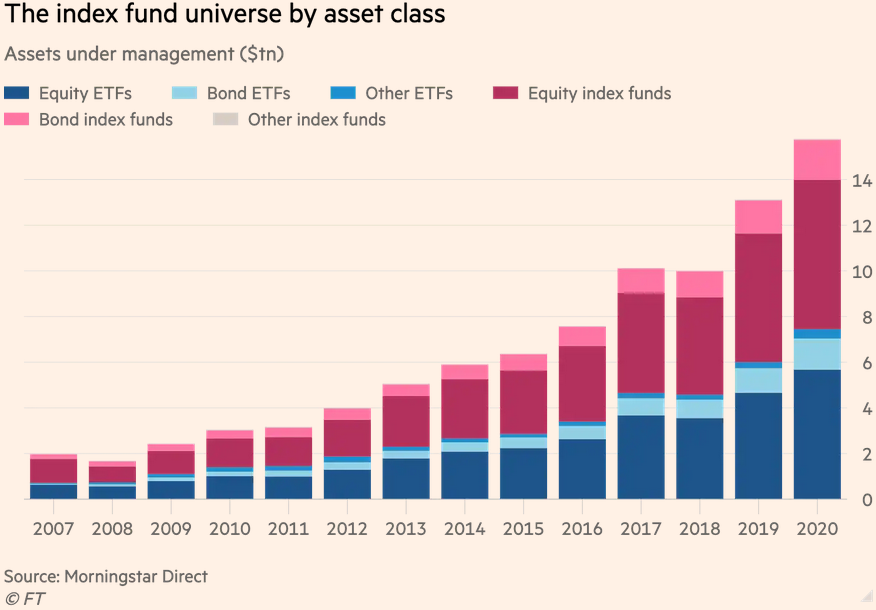
\includegraphics{fig/ft_index_funds_2007-2020.png}

\emph{Figure: FT}

\begin{verbatim}
Please use the sharing tools found via the share button at the top or side of articles. Copying articles to share with others is a breach of FT.com T&Cs and Copyright Policy. Email licensing@ft.com to buy additional rights. Subscribers may share up to 10 or 20 articles per month using the gift article service. More information can be found at https://www.ft.com/tour.
https://www.ft.com/content/7d5c2468-619c-4c4b-b3e7-b0da015e939d

Assets under management in exchange traded funds are eclipsing traditional index-tracking mutual funds for the first time, after the global passive investment industry vaulted past $15tn in assets last year.
\end{verbatim}

ETFs stood at \$7.71tn under management at the end of last year --- narrowly behind index mutual funds at \$7.76tn --- according to data compiled for the FT by the Investment Company Institute.

Since then, ETFs are likely to have nosed ahead thanks to powerful inflows this year. Comprehensive global data comes with a lag, but consultancy ETFGI calculates that assets under management in ETFs stood at \$8.33tn at the end of March.

The ascent of ETFs past their older cousins reflects the speed at which they have reshaped the investment industry.

``People are increasingly building entire investment strategies using only ETFs. The choices you have vastly outstrip what you have in traditional index funds,'' said Todd Rosenbluth, head of ETF and mutual fund research at CFRA.

Traditional passive mutual funds accept investor money or redemptions at the end of each day, whereas ETFs, first invented two decades later in the 1990s, trade like stocks on an exchange, letting investors hop in and out whenever they want.

The pandemic-triggered market upheaval of March 2020 failed to dent their growth, with bond ETFs now also quickly gaining ground among investors who were pleasantly surprised by their resilience in the turmoil.

Not everyone in the industry has been thrilled by the dramatic rise of ETFs. Some critics worry they lead investors to overtrade, which harms returns and exacerbates the volatility of markets.

Jack Bogle, the founder of Vanguard, introduced the first index mutual fund for ordinary savers, but was infamously hostile to ETFs and disliked when his old company entered the industry after he retired. However, he conceded before he died in 2019 that ETFs had changed ``not only the nature of indexing, but also the entire field of investing''.

Others argue that the flexibility of ETFs means securities that would normally be unavailable to ordinary investors --- such as complex derivatives --- can be easily packaged and sold to everyone without any restrictions.

\href{https://www.ft.com/content/7d5c2468-619c-4c4b-b3e7-b0da015e939d}{FT}

\hypertarget{big-three}{%
\section{Big Three}\label{big-three}}

\emph{Fitchner Abstract}

Since 2008, a massive shift has occurred from active toward passive investment strategies. The passive index fund industry is dominated by BlackRock, Vanguard, and State Street, which we call the ``Big Three.'' We comprehensively map the ownership of the Big Three in the United States and find that together they constitute the largest shareholder in 88 percent of the S\&P 500 firms. In contrast to active funds, the Big Three hold relatively illiquid and permanent ownership positions. This has led to opposing views on incentives and possibilities to actively exert shareholder power. Some argue passive investors have little shareholder power because they cannot ``exit,'' while others point out this gives them stronger incentives to actively influence corporations. Through an analysis of proxy vote records we find that the Big Three do utilize coordinated voting strategies and hence follow a centralized corporate governance strategy. However, they generally vote with management, except at director (re-)elections. Moreover, the Big Three may exert ``hidden power'' through two channels: First, via private engagements with management of invested companies; and second, because company executives could be prone to internalizing the objectives of the Big Three. We discuss how this development entails new forms of financial risk.

\hypertarget{the-age-of-asset-management-capitalism}{%
\subsection{The age of asset management capitalism}\label{the-age-of-asset-management-capitalism}}

\emph{Fitchner Memo}

In the early 1930s, Adolf Berle and Gardiner Means famously coined the phrase of the ``separation of ownership and control,'' meaning that there were not anymore blocks of ownership large enough to wield effective control over U.S. publicly listed corporations. 8 The dispersion of corporate ownership that Berle and Means observed empirically represented a markedly changed situation compared to the first decades of the twentieth century, when most large corporations had been owned and controlled by banks and bankers---what Rudolf Hilferding referred to as Finanzkapitalismus (finance capitalism). 9 Dispersed ownership however entailed that instead of the owners, it was the managers and directors who wielded control. This, in turn, led to the recognition of the principal-agent problem that underlies modern corporate governance theory: Given their collective action problem, how can the suppliers of capital (principals) ensure that the managers (agents) act in their best interests? In response to this question, corporate governance regulation has progressively shifted towards a more powerful position for shareholders. The extent to which the separation of ownership and control took shape has been a debate ever since. Nonetheless, there is an overwhelming consensus that since the second half of the twentieth century corporate ownership in the United States is by and large fragmented and dispersed.

Early signs of a fundamental change in the organization of corporate ownership emerged in the late twentieth century. Useem signaled the growing importance of mutual funds in the early 1990s and argued that we have moved from shareholder towards investor capitalism. 11 After the turn of the century and more than seven decades after Berle and Means, Davis went a step further and argued that the rapid rise of assets invested by actively managed mutual funds in equity markets and the ensuing re-concentration of corporate ownership led to a ``new finance capitalism.'' 12 Davis found that by 2005 active mutual funds had accumulated 5 percent blockholdings in hundreds of publicly listed U.S. companies. Being the single largest shareholder thus gave the biggest mutual funds---such as his running example Fidelity---potential power over the corporate governance of these listed companies by means of dominating corporate elections.

However, despite this great potential power, actively managed mutual funds at that time did not seek to influence corporate decision-making. Davis mentions three reasons for this. First, he points out that owners holding more than 10 percent of voting rights are considered as ``insiders,'' which significantly restricts their trading possibilities. Second, actively managed mutual funds are faced with potential conflicts of interest because the firms they are invested in are often also their clients. Particularly eminent is this where mutual funds are large providers of pension fund management for corporations. This curbs the willingness of funds to pursue shareholder activism. 13 Third, and more general, shareholder activism is always costly---and the costs are borne only by the activist, while the benefits are enjoyed by all shareholders. Hence, Davis concluded that ``networks of concentrated yet liquid ownership without control seem to be the distinctive feature of the new finance capitalism.'' 14 Davis pointed out that this observed new finance capitalism is historically unique, but also cautiously concluded that its durability remains to be seen. One decade later, we can safely conclude that the re-concentration of corporate ownership was not a temporary market anomaly, but a fundamental reorganization of the system of corporate governance. However, the period 2005--15 is also one of significant transformation of the new finance capitalism.

A remarkable feature of the passive index fund industry is its high level of concentration. In the ETF segment, the market shares in December 2016 have been 37 percent for BlackRock, 18.5 percent for Vanguard, and 15.5 percent for State Street, respectively. 20 Hence, together these three firms stand for a stunning 71 percent of the entire ETF market; all other ETF providers have market shares below 3.3 percent. Data about market shares in index mutual funds are not publicly available, but it seems clear that Vanguard dominates this segment with probably at least 75 percent market share.

BlackRock, Vanguard, and State Street dominate the passive index fund industry. Together they manage over 90 percent of all Assets under Management (AuM) in passive equity funds.

Although the Big Three have in common that they are passive asset managers, they are quite different in their own corporate governance structures. BlackRock is the largest of the Big Three---and represents the biggest asset manager in the world. At mid-2016, BlackRock had U.S. \$4.5 trillion in assets under management. 23 BlackRock is a publicly listed corporation and thus finds itself under pressure to maximize profits for its shareholders. Vanguard---with U.S. \$3.6 trillion in assets under management in mid-2016---is currently the fastest growing asset manager of the Big Three. In 2015, the group had inflows of U.S. \$236 billion, the largest annual flow of money to an asset managing company of all-time. 24 The main reason for the high growth of Vanguard is that it has the lowest fee-structure in the entire asset management industry. Vanguard is mutually owned by its individual funds and thus ultimately by the investors in these funds. Consequently, the group does not strive to maximize profits for external shareholders but instead operates ``at-cost,'' which allows Vanguard to offer the lowest fees in the industry. Vanguard pioneered passive investing by creating the ``First Index Investment Trust'' in 1975, however this investment approach was attacked as ``un-American'' at the time. 25 State Street is slightly smaller than BlackRock and Vanguard, but still one of the largest global asset managers. In mid-2016, it had U.S. \$2.3 trillion in assets under management.

A passive investment strategy leads to the question of why passive investors would be interested at all to concern themselves with corporate governance at the level of individual firms. If a fund holds---for instance---500 stocks the risk of any individual stock will be irrelevant. Indeed the incentive structure of passive index fund managers is such that they are rewarded more for keeping the costs low than for improving firm governance.

The decentralized attribution of ownership in separate funds and ETFs may hamper a centralized voting strategy in at least two ways. BlackRock for instance has more than 200 mutual funds and equity ETFs as well as several closed end equity funds and hedge funds---all of which could have positions in a particular firm. These portfolios may have different interests when it comes to shareholder vote. Even more differences occur because BlackRock holds some shares in short positions. Any vote that helps the long positions in BlackRock will hurt the short positions. So which way will BlackRock vote? These decentralized ownership structures may also hamper the ability to systematically use the voting power at all as it demands a serious coordination effort on behalf of the asset managers.

The risks of individual stocks are largely irrelevant to their business model.

While active investors can and will sell shares when they observe or anticipate diminishing (future) returns, passive investors are generally ``stuck.'' This means that their main interest is not short or medium term value creation, as is the case for most investors. Instead, their main interest is in long-term value creation.

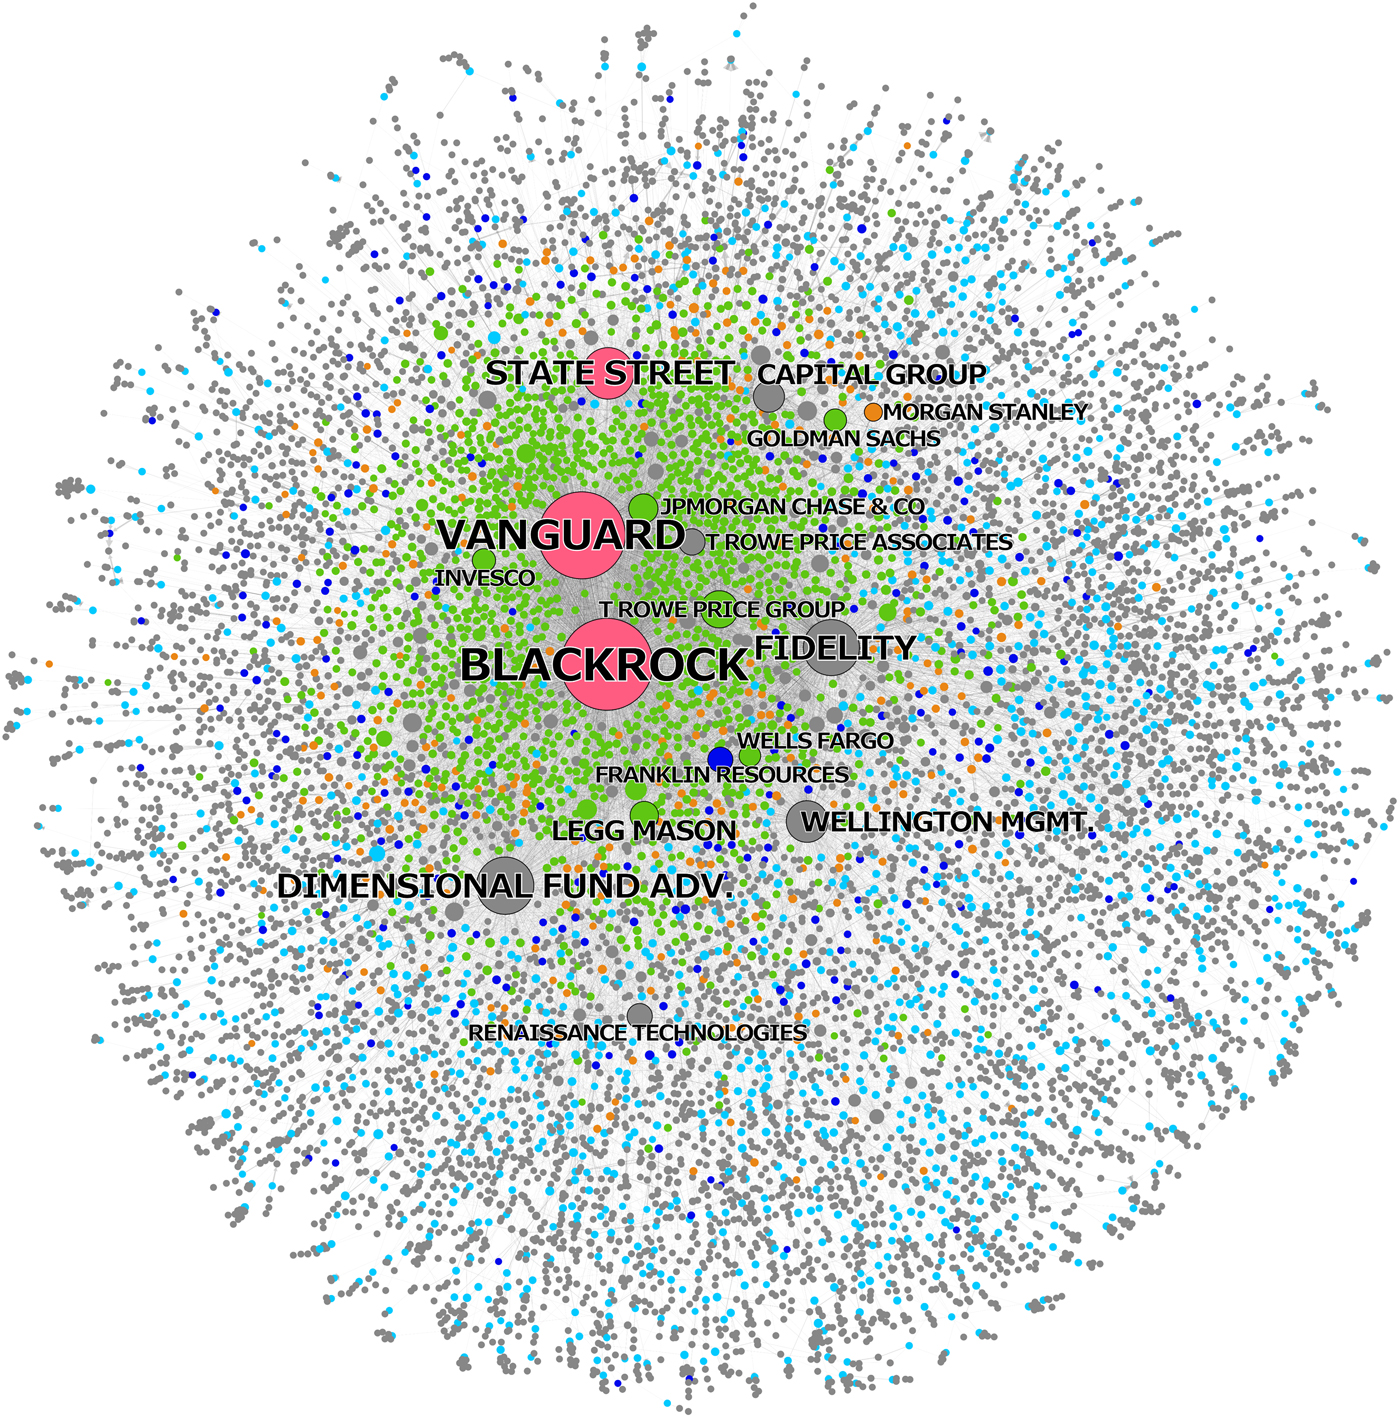
\includegraphics{fig/big3_ownership_map.jpeg}

\textbf{Asset management capitalism and new financial risk}

\emph{Stealth Socialism}

The recent rise of the Big Three has already led to serious concerns that ``it cannot be good for capitalism.'' 59 A first and major concern is that a further increasing market share of passive index funds could impair efficient price finding on equity markets, as the proportion of actively traded shares would continue to shrink. This concern already led some to polemically argue that because passive funds take active fund managers out of the role of allocating capital, the outcome is ``stealth socialism.'' 60 One of the most outspoken regulators concerning this topic is Andrew Haldane from the Bank of England. In a speech in 2014, he argued that we have potentially entered the ``age of asset management'' due to enormous growth of assets under management in the last decades and the relative retreat of banks after the global financial crisis. 61 He sees indications that passive investing could increase investor herding and thus lead to more correlated movements of markets. In this way, passive index funds could intensify the pro-cyclicality of financial markets.

A second concern regarding increased risk relates to the practice of securities lending. Passive asset managers regularly lend out shares to short-sellers to generate additional income. According to Cetorelli, BlackRock has increased its securities lending operations significantly in recent years. Indemnification of securities on loan by BlackRock more than tripled from U.S. \$40 billion in 2012 to over U.S. \$130 billion in 2014, while for State Street the value was even U.S. \$320 billion one year before. 62 Such securities lending---like most activities of large passive asset managers---seems to be unproblematic in good times, but could impair liquidity significantly in times of serious market stress. These developments have led global regulators to examine whether large asset managers, such as BlackRock, should be labeled ``systemically-important financial institutions.''
On the other hand, concerns about reduced liquidity due to passive investment strategies may be moderated by the observation that ETFs themselves have become the object of active trading strategies.

The active trading of passive index funds may have far reaching consequences. When passive index funds do indeed become the main building blocks for active investment, we are confronted with a fundamental reorganization of contemporary corporate governance. Because the voting rights reside with the asset managers who supply the passive index funds, and because the passive index fund industry is concentrated in the hands of the Big Three, this effectively means that the separation of ownership and control may potentially come to an end. After all, the active investors who trade with the passive building blocks no longer have access to the voting rights. And the Big Three accumulate the voting rights without much concern for short-term considerations. What is more, their interests are not restricted to the well-being of any particular firm. As mentioned, passive index fund managers arguably have little interest in fierce competition between their co-owned corporations, because this constitutes a zero-sum (or even negative-sum) game for them. Rather, they have industry or market-wide interests. Such developments may lead to a situation where the large owners of corporate businesses have limited incentives to engage with firm-level corporate governance beyond fulfilling their fiduciary obligations.

\emph{Fitchner Conclusion}

Since 2008, an unprecedented shift has occurred from active towards passive investment strategies. We showed that the passive index fund industry is dominated by BlackRock, Vanguard, and State Street. Seen together, these three giant, passive asset managers already constitute the largest shareholder in at least 40 percent of all U.S. listed companies and 88 percent of the S\&P 500 firms. Hence, the Big Three, through their corporate governance activities, could already be seen as the new ``de facto permanent governing board'' for over 40 percent of all listed U.S. corporations. 65

An original and compressive mapping of blockholdings revealed that in the United States the market for corporate control shows unprecedented levels of concentrated corporate ownership. The Big Three occupy a position of ``structural prominence'' in this network of corporate governance. We furthermore found that while the proxy voting strategies of the Big Three show signs of coordination, they by and large support management. However, BlackRock, Vanguard, and State Street may be able to influence management through private engagements. Moreover, management of co-owned companies are well aware that the Big Three are permanently invested in them, which makes it possible that through this ``disciplinary'' effect they may internalize some common objectives of the passive index managers. On balance, we find significant indications that the Big Three might be able to exert forms of power over the companies held in their portfolios that are hidden from direct inspection.

When Vanguard pioneered its index fund concept in the mid-1970s it was attacked as ``un-American,'' exactly because they held shares in all the firms of an index and did not try to find the companies that would perform best. Therefore, the new tripartite governing board of BlackRock, Vanguard, and State Street is potentially conflicting with the image of America as a very liberal market economy, in which corporations compete vigorously, ownership is generally fragmented, and capital is generally seen as ``impatient.'' 66 Benjamin Braun has argued that passive investors may, in principle, act as ``patient'' capital and thus facilitate long-term strategies. 67 Hence, the Big Three have the potential to cause significant change to the political economy of the United States, including through influencing important topics for corporations, such as short-termism versus long-termism, the (in)adequacy of management remuneration, and mergers and acquisitions.

We reflected on a number of anticompetitive effects that come with the rise of passive asset management, which could have negative consequences for economic growth and even for economic equality. As well, we signaled how the continuing growth of ETFs and other passive index funds can create new financial risk, including increased investor herding and greater volatility in times of severe financial instabilities. The ongoing rise of the Big Three and the concomitant fundamental transformation of corporate ownership today clearly warrants more research to examine their impact on financial markets and corporate control---in the United States but also internationally.

\href{https://www.cambridge.org/core/journals/business-and-politics/article/hidden-power-of-the-big-three-passive-index-funds-reconcentration-of-corporate-ownership-and-new-financial-risk/30AD689509AAD62F5B677E916C28C4B6}{Fitchner (2017) Hidden power of the Big Three? Passive index funds, re-concentration of corporate ownership, and new financial risk}

\hypertarget{shareholder-democracy}{%
\section{Shareholder Democracy}\label{shareholder-democracy}}

\emph{Sommer}

\begin{quote}
Control of most public companies ---
that is, the wealthiest organizations in the world,
with more revenue than most states ---
will soon be concentrated in the hands of a dozen or fewer people.
\end{quote}

In the near future, giant index funds, those low-cost investments that have helped millions of people to build nest eggs, will gain ``practical power over the majority of U.S. public companies.''
That nightmarish vision originated in a prescient 2018 paper by John Coates.

Index funds, which simply track the market and make no attempt to outperform it, are so effective and cheap, he said, that they have become the investment vehicle of choice for trillions of dollars of assets. Yet under current rules, it is the index fund executives, not the millions of people who invest in them, who have the power to cast proxy votes.

That lack of proxy voting capability leaves vast numbers of investors out of the equation, and gives corporations inordinate power.

When major fund companies receive compensation from corporations, they tend to side with corporate management even more frequently than usual.

The fundamental cure would be to take proxy voting power away from the fund companies and put it in the hands of millions of fund shareholders.

\href{https://www.nytimes.com/2021/05/21/business/stock-funds-shareholder-democracy.html}{Sommer (2021) Future True Shareholder Democracy}

\textbf{The Problem of Twelve}

\emph{Coates Abstract}

Three ongoing mega-trends are reshaping corporate governance: indexing, private equity, and globalization. These trends threaten to permanently entangle business with the state and create organizations controlled by a small number of individuals with unsurpassed power. The essay focuses on indexation. After providing background, the essay describes the rise of and reasons for indexation, noting that ``passive'' indexed investing takes a variety of forms. Data on indexation are presented --- with the bottom line that indexation has progressed farther than most realize, because foreign ownership, institutional indexation, and ``closet'' indexation are often neglected by observers. Index providers' incentives, resources, and methods are reviewed, with an emphasis on the how such providers have greater practical importance than simpler analytical approaches might suggest. The essay ends with an outline of policy options, and preliminary analyses of which seem likely to address the ``Problem of Twelve'' --- the likelihood that in the near future roughly twelve individuals will have practical power over the majority of U.S. public companies.

\href{https://papers.ssrn.com/sol3/papers.cfm?abstract_id=3247337}{Coates (2019) The Problem of Twelve}
\href{pdf/Coates_2019_The_Problem_of_Twelve.pdf}{(pdf)}

\hypertarget{direct-indexing}{%
\section{Direct Indexing}\label{direct-indexing}}

\emph{Planet Tracker}

An oligopoly of major index providers -- MSCI, FTSE Russell, S\&P Dow Jones and
Bloomberg -- are being challenged by innovative competitors. The index `majors' are
some of the most powerful players in the financial markets. If the drive towards self-
indexing continues -- and financial institutions have been positioning themselves for
such a move -- investors of all types will be able to choose from a much wider range of
products.
The sustainable investor could be the catalyst for this change, providing them with
the opportunity to invest in line with their personal principles, rather than taking
the templates on offer. And for the braver ones, direct indexing is becoming more
widespread. As for the corporates, being included in a popular sustainable index could
provide them with a cost of capital advantage. Things are looking up for sustainable
investors and sustainable companies

The index production landscape is evolving to meet the demands of
sustainability-based investment products. Declining fund fees, rising
competition in index production and demand for greater consumer
choice have all arrived at the same time as the upswing in sustainable
investing.

There are four main index providers for ETFs -- MSCI, FTSE Russell, S\&P Dow Jones and Bloomberg.
There is also another tier of index providers across asset classes which
are challenging this oligopoly.
These include CRSP, Morningstar, Qontigo and Solactive.

Solactive sells `tailormade' solutions as well as being `dedicated to developing
customized indices'.
Growing competition also exists from industry participants, including asset
managers and investment banks, that create their own indexes'

MSCI reveals dependency on the largest financial institutions with
BlackRock accounting `for 11.0\% of our total revenues'.

Two interesting examples of notable increases in
index demand: fixed income and ESG (environmental, social and governance).
In 2019, fixed income indices rose 7\% year-on-year, driven by Europe,
the Middle East and Africa (EMEA).
ESG indices rose by 14\% across both equities and fixed income.
The IIA snapshot for 2020 reveals continued growth in
fixed income indices of 7\% but a leap in ESG demand by 40\%.

ESG investing is `the growth opportunity of the century'.

If we then move the trillions of dollars of money away
from traditional indexes into these more sustainable or ESG-based indexes, that's going to
shape finance in a substantial way.

Testing further customisation
with STOXX iStudio, which provides the customer with the tools to build their own index.
This suggests Deutsche Börse is willing to become a disruptor.

So, are the index majors caught between a rock and a hard place? If they provide ever more
customisation, they undermine the profitability of their existing business model, especially in relation
to their most popular indices -- e.g.~S\&P 500, FTSE 100, MSCI World etc.
But there's a further issue. Will increasing customisation, driven by sustainable demand, lead to
greater regulatory scrutiny? Some regulators have already expressed concerns. In 2018, the EU
Benchmark Regulation (BMR) was introduced amid fears about the accuracy and integrity of indices
used as benchmarks in EU markets, following the LIBOR g scandal. BMR imposes requirements for
organizations that provide, contribute data to and reference financial benchmarks. 30 To further
complicate the issue, regulators will need to ensure that the largest Asset Managers, which may sit
on Advisory Boards of the Index Providers or provide advice, are unable to exert influence over the
formulation of indices.

Index providers are viewed as data publishers by the SEC, rather than investment advisers. Should
there be a regulatory distinction between broad indices and the customised varieties?

Presently, it appears that only financial institutions and ultra-high net worth individuals (UHNWIs)
are reaping the full customisation benefits. Many retail investors are left with limited options when
using the fund platforms of the major financial institutions.

Perhaps the most exciting development for supporters of sustainability and ESG strategies may be
an unintended consequence. If corporate management teams become convinced that the inclusion
of their company in an index is one of the most important drivers of a share price, then there could
be a scramble by executives to adopt more sustainable and ESG strategies, in order to win access to
these indices and possibly lower their cost of capital. A race to the top that would be welcomed by
many.

\href{https://planet-tracker.org/tracker-programmes/cross-programme-papers/\#indexing-prepare-for-sustainability-driven-disruption}{Planet Tracker (2021) Sustainability-Driven Disruption}
\href{pdf/Planettracker_2021_Indexing.pdf}{(pdf)}
\href{https://planet-tracker.org/large-index-providers-should-prepare-for-disruption-says-planet-tracker/}{Press Release}

\hypertarget{institutional-investors-1}{%
\chapter{Institutional Investors}\label{institutional-investors-1}}

\hypertarget{pension-funds}{%
\section{Pension Funds}\label{pension-funds}}

\emph{Braun}

Rather than
financing entrepreneurs and fostering growth,
pension money has ``{[}inflated{]} capital markets in
which unproductive takeover and corporate
restructuring activity flourishes, while industrial
production and employment activity stagnate.''

At the same time, their capital feeds an asset
management sector geared toward capitalizing an
ever-increasing share of economic activity, thus
expanding the universe of investable assets.

It is ``never noticed'' by advocates
of market provision ``that financial markets are
not large enough to support welfare transfers.''

Invariably, therefore, the supply of pension sav-
ings in search of investment outstrips demand
for financing from the non-financial sector
(firms, households, government). This mis-
match means that pension capital contributes to
asset price inflation and to declining yields in
established, ``conservative'' asset classes, which
in turn gives pension funds a strong incentive to
lobby state and federal governments to allow
them to move into high-risk investment strate-
gies and asset classes. In this effort, they will
invariably be supported by the asset manage-
ment sector.

Pension funds' asset composition has steadily
moved from public, local, and development-
oriented investments to more private, global,
and predatory investments.

In a system in
which financial return is structurally linked to
predation, exercising labor power through capi-
tal stewardship is doomed to fail. Unlocking the
progressive promise of labor's capital requires
a macro-financial regime that strictly regulates
finance and that allows for greater economic
democracy. The public would play a much
greater role in credit creation and allocation,
labor's capital would be uncoupled from
the for-profit asset management sector, and
employee equity funds and other forms of
mutual ownership would institutionalize profit-
sharing and co-determination at the firm level. 35
On the transition path to such a ``real utopia,''
funded pensions appear as an obstacle rather
than a stepping stone because they create a
sequencing problem---things would have to get
worse for labor's capital before they get better
for labor.

\href{pdf/Braun_2021_Fueling_Financialization_Funded_Pensions.pdf}{Braun (2021) Fueling Financialization: The Economic Consequences of Funded Pensions (pdf)}

\hypertarget{esg-2.0-1}{%
\section{ESG 2.0}\label{esg-2.0-1}}

\emph{Segal}

\textbf{How Institutional Investors Encourage Corporations Bad Behavior}

Wittingly or unwittingly, pensions and endowments' investment strategies aid and abet activities that make the financial system more fragile.

The growing scale of institutions and the large amounts of money they need to deploy into high-risk investments is leading to consolidation among asset managers, higher global debt levels, short-term corporate behavior, and market instability.

Institutions' investment strategies are in conflict with environmental, social, and governance goals to which they are increasingly committing.

Pension funds, insurance companies, sovereign wealth funds and others need to deploy large amounts of capital efficiently because they themselves are so big.

Institutions' only option in many cases is to put billions of dollars to work in the largest public and private companies, Rothenberg explained. That results in companies, for example, taking on unsustainable amounts of debt.

There are incentives to layer on debt, much of which is supplied by capital markets and the shadow banking sector.

Ironically, institutional investors want to integrate ESG into their process, but they also contribute to corporate consolidation and huge debt burdens. Institutional investors are essentially contributing to some of their own problems in the way they allocate capital to leveraged loans, high-yield loans, collateralized loan obligations
and other higher risk products.

All of this adds to global systemic risks.
Unchecked increases in corporate debt result in increased systematic market risk that boomerangs back to investors and their portfolios
Existing approaches like Modern Portfolio Theory and ESG or impact investing frameworks don't focus on these potentially negative effects.

Perversely, as major central banks globally respond to the current crisis with rock bottom interest rates and new rounds of quantitative easing (QE), investors and companies are further incentivized to increase their exposure to high-risk debt and inflated asset valuations --- a situation that leaves society and markets vulnerable to a rise in interest rates or other unplanned challenges

\href{https://www.institutionalinvestor.com/article/b1r9js87jhyn8s/How-Institutional-Investors-Encourage-Corporations-Bad-Behavior}{Segal - Comment - Instititional Investor}

\emph{Rothenburg}

Many of our existing ESG and impact investing frameworks focus on issues at the
portfolio company level, but they do not take into account potential negative
impacts from capital structures and investors' influence in shaping them.
Asset allocation strategies can be in conflict with ESG objectives.

The conflict materializes in various interconnected ways, particularly from
institutional investors' role in increasing global debt levels and
fund manager and corporate consolidation.

For long-term, diversified institutional investors, or ``Universal Owners''
of the market, these dynamics eventually translate into lower financial returns.
For workers and communities, these dynamics translate into
greater precarity and inequality.

Potential solutions focus on diversifying asset allocation to
more regenerative investment structures and asset classes, building an
enabling environment through adjustments to team incentive structures, performance reviews,
benchmarking and valuation methodologies, and field-building.

Over the past decades, institutional investors have migrated up
the risk-return spectrum to asset classes with higher yields.
Investor allocations to private equity (PE), venture capital (VC), private debt (PD),
high yield bonds (HYBs), leveraged loans (LLs), and
collateralized loan obligations (CLOs), for instance,
have been growing steadily in response to a number of trends.
\emph{While such shifts in asset allocation may suit near-term goals,
such as meeting actuarial targets, this institutional allocation to higher risk asset
classes has also meant increased global debt burdens, corporate and
fund manager consolidation, and risk across capital structures,
resulting in fragility for companies, the real economy, and the stability of
financial markets.
The resulting risks are therefore shared not only by investors,
but also governments,workers, and communities alike.}

To optimize leverage ratios, companies may prioritize debt servicing or distributions to investors at the
expense of worker payrolls and benefits. Infrastructure and social infrastructure investments --- such as
power, water, roads, hospitals, nursing homes, housing, and cybersecurity --- might be structured in
such a way that provides access to end-users at unaffordable prices, or of poor quality, in order to meet
investor return expectations and therefore attract capital. Weak capital structures increase the risk of
restructurings or bankruptcies that are detrimental for stakeholders, such as workers. Stakeholders have
increasingly raised concerns about high leverage, coined ``financial engineering,'' particularly in the PE
asset class, for such reasons. 5 Yet studies produced over the past decades, inspired by PE, praise the
discipline of debt, and due to a number of additional factors, high leverage ratios are no longer confined
to the PE asset class and are prolific across public equity markets, as well.

In practice, the negative impacts of weak capital structures are typically being addressed piecemeal
through company-by-company interventions that focus on corporate operations, like a game of whack-
a-mole; but key roots of the problem --- the investment structures themselves --- are left unaddressed.

The unintended negative consequences of highly levered investments have been underexplored when it
comes to ESG and impact investing frameworks and practice. Matters relating to investment structures,
capital structures, leverage ratios, earnings calculations, valuation methodologies, benchmarking
approaches, and resulting asset allocation and portfolio construction are not typically within the realm
of ESG-related responsibilities.

Too much leverage is dangerous for all stakeholders.
While leverage looks like a neutral, bilateral accelerant, it
actually reduces financial resiliency at the very times when it might be most needed.

Systemic inequality has been shown to result in economic decline.

Neither Modern Portfolio Theory (MPT) nor ESG or impact investing frameworks
currently include a focus on potential negative impacts stemming from
investment structures.

Corporate debt burdens and leverage ratios are historically high, covenants are light, and
defaults and bankruptcies are being held at bay by government support
(e.g.~through fiscal and monetary policy) -- which is also funded by debt,
though at the sovereign level.

Corporate funding dynamics have changed since the Global Financial Crisis
(GFC), when banks came under heavy regulation that caused them to
restrict lending to smaller clients.
Capital markets, or the Non-bank Financial Intermediary
(``NBFI'' or ``Shadow Banking'') sector, has stepped in to fill this void.

The financial assets of the NBFI sector amounted to \$200.2 trillion in 2019,
accounting for nearly half of the global financial system in 2019, up from 42\%
in 2008

\emph{How Did We Get Here?}

For the past two decades, institutional asset owners have significantly shifted their overall asset
allocation strategy. Private markets -- including PE, PD, VC, infrastructure, and real estate - as well as LLs,
CLOs, and HYBs, have become much larger percentages of overall portfolios. There are a number of
reasons for these changes, including, but not limited to, ongoing declines in interest rates by major
global central banks, dynamics related to funding ratios of institutional investors such as pension funds,
growing interest in the illiquidity premium of private markets, benchmarking practices, investor
dissatisfaction with public markets, and increased opportunity for NBFIs to provide financing following
banking regulations resulting from the GFC. 16 Private capital assets under management (AUM) in 2019
was approximately US\$6.5 trillion, an increase of over US\$4 trillion over the past ten years.

\emph{Private Equity (PE)}

Investor demand is now so high for PE that many are concerned that the asset class is becoming crowded with capital.

Consolidated capital flows stems from the institutionalization of capital.
Markets have evolved from being dominated by individual investors to
having a large presence of institutional investors.
Institutional investors now hold over 40 percent of
global market capitalization of listed companies.

Institutional investors have sizable portfolios and must invest billions
if not trillions of dollars.
With such large chunks of capital to put to work,
they often find it challenging to invest in smaller fund managers,
smaller companies, and niche investment strategies due to a number of factors,
such as transaction costs.

Even when small deals perform well, which data suggests that they often do,
they are hard to justify because they do not meaningfully move the needle
in terms of overall portfolio returns.

A well-documented negative impact of consolidated capital flows to larger
fund managers is that
smaller, emerging, and innovative fund managers can be starved of capital.

\emph{Institutionalization of Capital}

The consolidation of capital among institutional investors is a double-edged sword. On the one hand,
institutions offer individual investors professional money management with multi-disciplinary staff and
robust internal infrastructure capable of constructing well-diversified portfolios. Size and scale can also allow
large allocators to influence corporate governance of portfolio companies, as well as negotiate more
attractive terms with fund managers. It is arguable that fees overall are reduced through these dynamics, and
strong ESG practices can be better advocated for. On the other hand, since large institutions need to put
significant amounts of capital to work, they often allocate to the largest managers and companies, thereby
resulting in consolidation of power, profit, influence, and opportunity among a shrinking pool of asset
managers and companies. 53 In order for large institutional investors to act as responsible Universal Owners
and effectively manage systematic risk, it will be critical for them to evaluate their asset allocation practices
for unintended negative consequences that not only impact the real economy, but also markets and their
long-term portfolios.

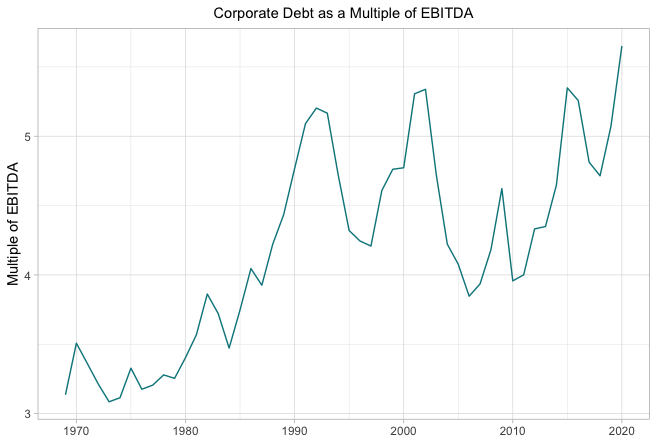
\includegraphics{fig/corporate_debt_ebitda.png}

This high-risk debt is not limited to private companies. A recent Forbes article highlights how, ``some of
the biggest firms in the United States\ldots{} have binged on low interest debt. Most of them borrowed more
than they needed, often returning it to shareholders in the form of buybacks and dividends. They also
went on acquisition sprees.''

From the corporate perspective, historically cheap credit due to low interest rates is attractive,
particularly when combined with the current tax deductibility of interest expense, studies suggesting
that highly leveraged capital structures do not negatively impact stock prices, and arguments that debt
adds discipline to corporate management. Yet debt and common uses of funds can increase risk for
other stakeholders. M\&A has been shown to contribute to corporate consolidation which can stifle
SMEs, innovation, suppliers, the quality and affordability of goods and services, labor's bargaining
power, and diversification for institutional investors. There is significant literature that explores
negative impacts of share buybacks in public companies, given the links with high executive
compensation and that cash paid to executives and shareholders can deter from reinvestment in the
company, the quality of goods and services, and the workforce. In PE-backed companies, high leverage
from acquisitions and dividend recapitalizations can push companies to cut costs related to quality jobs
and jeopardize the quality and affordability of goods and services.

As central banks around the world doubled down on low interest rates and QE, investors responded by
increasing portfolio allocation to higher risk and yielding asset classes.

The combination of QE and low interest rates with corporate consolidation and high
inequality may well be creating challenges to long-term economic growth,
as well as introducing
potential drivers of instability for aggregate demand.

\href{https://papers.ssrn.com/sol3/papers.cfm?abstract_id=3820316}{Rothenberg (2021) ESG 2.0 - Measuring \& Managing Investor Risks Beyond the Enterprise-level}
\href{Rothenberg_2021_ESG2.pdf}{(pdf)}

\hypertarget{capital-markets}{%
\chapter{Capital Markets}\label{capital-markets}}

\hypertarget{china}{%
\section{China}\label{china}}

\emph{Petry Abstract}

Since 2009, China's capital markets have developed and internationalized to an unprecedented
degree, which has contributed to a lot of debates on China's rise and its implications for the
global financial order. Contributing to these debates, this article analyses the development of
capital markets in China and their integration into global finance between 2009 and 2019, focusing
on three aspects: how Chinese capital markets are developing domestically; how they are inte-
grating with global markets; and how Chinese capital markets are internationalizing, i.e.~expanding
abroad. Thereby, the article analyses the crucial role of securities exchanges who as organizers of
capital markets are powerful actors that exercise considerable influence over these markets and
their development. This empirical investigation reveals that while they share some characteristics
with `global' capital markets, Chinese capital markets function quite differently. The article argues
that China's state-owned exchanges facilitate the development of state-capitalist capital markets --
capital markets that follow an institutional logic derived from China's state-capitalist economic
system. Rather than giving in to a neoliberal rulebook, China's capital markets represent an
alternative to, resist and challenge the norms, principles and procedures of the contemporary
global financial order. While different capital markets share some characteristics, they are insti-
tutionally embedded, and these institutional settings facilitate different institutional logics that
underpin and inform the functioning of markets. Instead of viewing capital markets as homoge-
neous entities, the article therefore proposes to investigate a `varieties of capital markets' that are
shaped by different institutional logics.

\emph{Petry Memo}

In 1989, capital markets did not exist in China. Fast forward three decades, China's capital
markets have become the second largest equity markets, second largest futures markets and
third largest bond markets globally.

While China's markets had been virtually
closed from the outside world for decades, especially since the global financial crisis (GFC)
2007--2009, they have become connected to both regional and global financial markets `at an
unprecedented pace'.

This growing Chinese significance in global finance
is also expressed by the internationalization of the renminbi,
how their investments change financing patterns,
China's growing
role in development finance and global financial governance,
and with the Belt-and-Road Initiative (BRI).

The rapid growth of China's capital markets takes place within the context of a global
financial order (GFO) based on neoliberal principles of open, lightly-regulated, internation-
ally-integrated financial markets, guaranteed and facilitated by US power.
Scholars are therefore debating whether China is a
status quo power integrating into the GFO,
a reforming power,
a revisionist power challenging this (neo)liberal, US-dominated financial order
or whether global finance is itself adapting to accommodate China.

This discussion is linked to broader debates on state capitalism,
where some policy makers fear that China will not play by the neoliberal
rulebook on which the contemporary global (financial) order is based.

In these debates, state capitalism is often
defined in juxtaposition to capital markets, the epitome of liberal capitalism.

By linking state capitalism, capital markets and the neoliberal GFO, this article contrib-
utes to these debates, seeking to make a twofold contribution. Empirically, the article anal-
yses the post-GFC reform and opening process of China's capital markets between 2009 and
2019. This empirical investigation reveals that capital markets in China function
significantly different from `global' markets. While many Western commentators argue
that `proper'
capital markets do not exist in China, this article argues that such assessments actually
reflect the neoliberal bias that Western views of markets exhibit, thereby shedding light
on the contested politics between different types of capital markets championed by China
and the US. Theoretically, the article therefore proposes to re-evaluate common global
political economy (GPE) conceptions of capital markets: instead of viewing these as uniform
entities, in opposition to the state and interlinked with the concept of neoliberalism, to look
at an institutionally embedded `varieties of capital markets'.

In China one can observe the development of \emph{state-capitalist capital markets}
as Chinese capital markets are intricately linked with state institutions
and play an active role in facilitating national development goals.
The article examines the crucial role of China's (stock and derivatives) exchanges as
important actors who organize markets in a way that facilitates state-capitalist logic, shap-
ing capital market dynamics and directing market outcomes towards state objectives, both
within China and internationally. The capital markets organized by China's exchanges
thereby provide an alternative to, resist pressures to conform with, and even challenge
the neoliberal capital markets that underpin the GFO. In other words, no matter how
deep the reforms, Chinese capital markets will not converge with global markets but
rather maintain their distinct character.

As such, the capital markets underpinning
the GFO facilitate and perpetuate existing power relations and hierarchies within global
capitalism.
State capitalism is
often defined as the anti-thesis of such governance through markets, as the state's
predominance over markets and impairment of `free' market mechanisms.
Proponents of liberal, free markets argue that there might be state capitalism in China,
but not `true capitalism'.

Moving beyond the fact that states and capitalism have historically been in an intimate
relationship, state capitalism literature focuses on a more recent
empirical phenomenon -- the increasing intensity of government direction and steering in
economic processes, especially in emerging markets.

In contrast to earlier forms of state-led eco-
nomic development in the late-19th (US, Germany) and mid-20th century (Stalinism, fas-
cism, developmental states), contemporary state capitalism relies less on prohibitive tariffs
(first wave) or centralized command structures (second wave) but more on market-based
economic coordination which, however, is controlled, steered or influenced by the state.

State capitalism highlights `the essentially
capitalist nature of the {[}socio-economic{]} system' where markets are important but `the
state plays a very large role' through intervening into the economy and state-ownership.

While the Chinese state has recognized the usefulness of market-based mechanisms for
economic coordination, `free' markets are seen as something not quite to be
trusted, endogenously crisis-prone, socially unproductive and leading to a loss of control
over the economic system if not strictly regulated.
The state rather
engages in a `pragmatic use' of markets, managing markets for specific policy goals.

State-owned banks are the main actors in China's financial system.
State capitalism is often understood in juxtaposition to capital markets, the epitome of
liberal capitalism. However, capital markets have become more important in China since
the GFC.

In GPE literature,
states and markets have long been analysed as opposing institutions prevailing over or
constraining each other's actions.
While the role of states
in promoting capital markets has been well-documented and more recently
a focus has emerged around `governing through financial markets',
capital markets and their organization are often conceptualized as uniform, and divergencies
between markets and the sources of these differences are seldom the focus of GPE analyses.

In the comparative capitalism literature, state and market are also defined as
mutually exclusive for economic coordination within national economies.

Especially with regard to the financial system,
either the state facilitates credit provision, mainly through state-owned and policy-banks,
or market relations fulfil this role. Markets are coordination mechanisms
that result from certain institutional arrangements -- but capital markets themselves are
often conceptualized as homogenous, with little internal variegation.

If not all markets are equal,
they might produce different outcomes and socio-economic effects. What is missing is a
better understanding of the differential organization of capital markets.

In contrast to the premise that markets are uniform, following the likes of Keynes and
Polanyi, economic sociology has shown that markets are `embedded in distinct sets of social
and political institutions'.
Markets are social phenomena that are
embedded in and influenced by man-made institutional arrangements.
How and by whom markets are organized matters. For capital markets, this function is
mainly fulfilled by securities exchanges.
Instead of mere institutions/platforms on which
market transactions take place, exchanges are powerful actors in their own right who active-
ly organize and shape capital markets.
`Power often depend{[}s{]} on control over key financial infrastructures' that enable
the functioning of financial markets.

Exchanges are such actors whose business is to orga-
nize, create and control their infrastructural arrangements. Rather than investors who are
active within markets, as infrastructure providers exchanges play a more architectural role
for capital markets. By deciding the `rules of the game' and acting as gatekeepers in capital
markets, deciding who gets in, what is traded and how trading is conducted, exchanges are
crucial in shaping capital markets.

But both capital markets and exchanges are embedded and shaped by their institutional
environment. These institutional configurations
create a particular contextual ``logic'' or rationality of economic action. Every economy
consists of a set of institutions which create distinct patterns of constraints and incentives
that shape and channel actors' behaviours (Zysman, 1994: 245--246). Hence, given the
existing institutional structure, a particular institutional logic emerges
that is distinct from
other institutional contexts. So, while functionally all capital
markets are characterized by market-based mechanisms of coordination between buyers,
sellers and investors, applying the concept of institutional logic to capital markets reveals
how the institutional embeddedness of markets and market organizers shapes these markets,
leading to different market dynamics and outcomes.

Consequently, how exchanges (i.e.~market organizers) are governed and which con-
straints and incentives they face matters. In the West, exchanges are publicly traded com-
panies that have to make profitable business decisions to increase shareholder value; they
are situated within an institutional setting informed by a neoliberal institutional logic.

Six global exchange groups (GEGs) dominate global capital markets: account-
ing for 50\% of exchange industry profits, futures trading volume and stock market
capitalization globally.

The ostensible purpose of these capital markets that underpin the neoliberal
GFO is to achieve `efficiency' by enabling the generation of (private) profit, which is
achieved by the principles of `free markets' and `free flows of capital' that should be respon-
sible for allocating economic resources without state intervention.

The underlying neoliberal institutional logic that informs the functioning of
these markets depoliticizes those
markets, proposes a (`supposed') separation between state and capital markets, and puts
a significant degree of trust and power in the collective agency of private (financial) capital
actors to achieve `efficient' outcomes by maximizing (private) profit.
While the state is not absent, its priority is enabling private profit creation
instead of other socio-economic outcomes, cementing the power of private finance capital.

Merely adopting market-
mechanisms (e.g.~capital markets) does not make China neoliberal. While market-based
finance emerged as an important economic governance tool in China (Gabor, 2018),
Chinese capital markets function fundamentally different than neoliberal capital markets.
This is because exchanges and capital markets are situated within a very different
institutional context -- that of state capitalism.
The institutional logic of China's state capitalism is
not simply one of command-and-control but a combination of top-down state coordination
and bottom-up market competition.

China's capitalism `relies on a unique duality or dialectic whereby state-
capitalist features are balanced by {[}. . .{]} a variety of hybrid institutional arrangements'
(also, Sum, 2019). Chinese capital markets also follow this institutional logic. Bottom-up
you have millions of profit-driven speculating investors that create manias, panics and
crashes like in any capital market. But while profit creation for private finance capital is
the primary underlying principle in neoliberal markets, importantly, in China, the state
intervenes into capital markets to steer them into `productive' tracks that facilitate state
objectives. The defining difference between neoliberal and state-capitalist logic is not the
existence of markets per se but rather the principles that underlie market organization
(profit creation vs state objectives) and the actors that dominate/shape these markets (pri-
vate finance capital vs state institutions).

While investors act as entrepreneurs, `certain levers of state control remain intact'.
As the organizers of capital markets, exchanges remain strictly in
government control.
These `infrastructural
arrangements {[}are important{]} because this is where you can control the market'. 5 The
exchanges are also deeply embedded in the \emph{nomenklatura system}; doing a
good job as senior exchange manager (i.e.~directing markets towards state policies)
is important for party officials to eventually get promoted to higher positions.
`The financial industry can therefore justifiably be treated as an integral part of the
political system'. In contrast to being `marketized', exchanges in China are rather `politi-
cized'. Therefore, capital markets can be understood as a site where the authorities exercise
`statecraft {[}through{]} financial control'.

Chinese exchanges organize
markets by designing market infrastructures that aim to shape market behaviour by mon-
itoring, regulating and managing the behaviour of market participants and direct market
outcomes towards the accomplishment of state objectives, both within China and abroad.
Rather than neoliberal, the capital markets organized by China's state-owned exchanges
should hence be conceptualized as \emph{state-capitalist capital markets}.

Neoliberal or state-capitalist,
they are both capital markets populated by profit-driven investors and prone to speculative
dynamics. However, what can be observed is that in China, a fundamentally different way of
thinking about, managing and governing capital markets has emerged, as these markets are
permeated by but also reproduce the institutional logic of Chinese state capitalism.

\begin{enumerate}
\def\labelenumi{\arabic{enumi}.}
\item
  Chinese exchanges develop markets that represent a \emph{distinct alternative} to neoliberal
  capital markets.
\item
  China's integration into global finance through its exchanges (largely) conforms
  with state-capitalist logic, demonstrating their resistance to conform with neoliberal
  capital markets.
\item
  Chinese capital markets not only resist
  but also challenge US-dominated neoliberal capital markets.
\end{enumerate}

The growing importance of market-based finance in China does not
represent a shift towards neoliberalism but rather a perpetuation of Chinese state capitalism
through financial means.

In 2017, Xi Jinping noted that the tasks of China's financial sector were
above all `{[}to{]} better serve the real economy!
Markets are organized to facilitate these policies.

The partially contradictory nature
of state-capitalist institutional logic. On the one hand, the state aims to control financial
instability, and on the other hand, it has interwoven social stability with capital market
participation which in turn potentially decreases financial stability

The exchanges' system of risk monitoring and management
is used in a delicate balancing act between allowing retail investors
to participate in markets but also reduce the volatility that they bring into markets, profes-
sionalize/educate them and protect them from themselves and more sophisticated investors.

China has an ambiguous relationship with foreign
investors. As one interviewee stated, `it's absolutely a love and hate story, they love the
money, love the stability, hate giving up control. . . and hate it if foreign investors want to
dominate the terms'.

Foreigners are not allowed to freely participate in Chinese markets but only if they
establish local entities, so-called wholly foreign-owned enterprises (WFOEs). 36 As several
interviewees noted, setting up WFOEs to trade in capital markets is accepted by the author-
ities -- because they are registered in China, subject to Chinese laws, funds/profits cannot be
easily repatriated, and they can be monitored and controlled by the Chinese exchanges.
One called China a `façade of an open market'.

`Step by step there is a whole market infrastructure
emerging' that connects China with the outside world. 50 But while China is increasingly
integrating with global finance, international investors have to play according to Chinese
rules. Attempts to shape market behaviour and steer market outcomes are maintained by
China's exchanges, following China's state-capitalist logic of organizing capital markets,
and demonstrating China's resistance to conform with neoliberal capital markets underpin-
ning the GFO.

In their current form, global markets are not perceived as fair but as being stacked against
Chinese interests, rather benefitting Western private financial actors.
Similar to RMB internationalization, the internationalization of China's capital mar-
kets is part of the state's strategy to change the rules of the game in global finance or at least
to create a level-playing field that does not disadvantage China.

This case study hence highlights the need to re-evaluate the conceptual toolbox with
which we analyse global finance. In political economy literature, capital markets are often
viewed as homogeneous entities, an analytical category different from/contrary to `the
state', and capital market development is often linked to a neoliberal policy paradigm.
However, as the findings of this article demonstrate, conceptually capital markets (and
exchanges) should be analysed separate from neoliberalism.

\href{https://journals.sagepub.com/doi/10.1177/1024529420964723}{Petry (2020) Same but different}
\href{pdf/Petry_2020_Same_but_different_China_Capital_Markets.pdf}{(pdf)}

\hypertarget{climate-finance}{%
\chapter{Climate Finance}\label{climate-finance}}

\hypertarget{institutional-dynamics}{%
\section{Institutional Dynamics}\label{institutional-dynamics}}

\emph{Baer}

Financial markets not only have an important role to play in steering financial capital to support the net-zero transition but also are increasingly vulnerable to climate-related financial risk that may be a source of financial instability. In this context, Frank Elderson, chair of the Network for Greening the Financial System, in a speech of 2018 meaningfully titled `Let's dance'

, highlighted the elevated responsibility of central banks to act on climate change.

Analysing the institutional relations between political authorities (governments) and delegated authorities (central banks and financial regulators), as well as their mandates and degree of freedom for intervention across jurisdictions, the authors of this paper argue that central banks cannot and should not `dance alone', as only coordinated efforts between these institutions will be sufficient to mitigate climate risks -- put simply, it takes two to dance.

Supporting the analysis and to better explain the heterogeneity in institutional behaviours in the field of climate-related financial policies, the authors propose a framework to distinguish: i) the motives for policy implementation -- either the desire to tackle climate change by directly influencing the allocation of financial capital (promotional) or the desire to ensure the stability of the financial system in the face of climate-related challenges (prudential); ii) the relevant policy instruments to achieve these objectives (informational, incentive and coercive); and iii) the type of implementing authority (political or delegated).

Applying this framework, the authors demonstrate how sustainable financial interventions in certain jurisdictions -- most notably, the EU -- rely solely on informational policies to achieve both promotional and prudential objectives; this is in contrast to emerging economies. The authors term this restricted usage of climate-related financial policies for promotional purposes in Europe a `promotional gap' and explain this through two main institutional dimensions: the low strength of public control on private financial markets; and the high degree of independence of delegated authorities. This leads to an institutional deadlock in which only measures fitting with both political and delegated authorities' objectives can be implemented.

Relying on a game-theoretic framework, the authors then argue that the current institutional setting is unstable and discuss three potential evolutions: a drift towards a green financial technocracy; a re-politicisation of delegated authorities; or a move towards fiscal-monetary coordination.

\href{https://www.lse.ac.uk/granthaminstitute/publication/it-takes-two-to-dance-institutional-dynamics-and-climate-related-financial-policies/}{Baer}
\href{pdf/Baer_2021_Institutional_Climate_Policy_Dynamics.pdf}{(pdf)}

\hypertarget{assistance-to-developing-countries}{%
\section{Assistance to Developing Countries}\label{assistance-to-developing-countries}}

Climate Finance assistance to developing countries is NOT on track.
\href{news.html\#climate-finance-shadow-report-2020}{Oxfam Report 2020 (News issue)}

\hypertarget{asset-managers-scoreboard}{%
\section{Asset Managers' Scoreboard}\label{asset-managers-scoreboard}}

We surveyed 29 major asset managers, mostly based in Europe
and among the biggest institutions in terms of assets
under management. We analyzed their investment practices
regarding climate change, using coal as the most straightforward
benchmark on climate. The first edition of this scorecard focuses on
coal, as one of the easiest asset classes financial institutions can begin
to act on and as the sector that requires the most urgent exit.

Key information on our sample of 29 asset managers:

• They represent a total of €34 trillion in assets under
management;

• Overall, `passively' managed assets represent approximately
48\% of this amount;

• Each participant represents at least €300 billion in assets
under management and 24 participants are headquartered
in Europe.

Main findings:

• Less than half of the asset managers assessed have a public policy to phase
out coal. Vanguard, PIMCO and Schroders are among the big asset managers
that have still not adopted such a policy.

• Moreover, because these policies often allow for many exceptions, overall,
only 25\% of all the assets managed within our sample were covered by a
coal exclusion criterion. For example, while they have adopted a coal policy,
BlackRock, Legal \& General Investment Management and UBS AM's coal
policies apply to less than 40 \% of their assets.

• Even when a coal policy does apply, the criteria used to exclude companies
are rarely robust. Only 20\% of the asset managers exclude companies that
still have coal expansion plans. As a result, of €23 trillion of assets covered by
long term climate commitments, only €3.4 trillion exclude companies with
coal expansion plans.

• Even worse, whilst being signatories of the Net Zero Asset Managers
Initiative, six asset managers have still not adopted any public policy to
restrict investments in coal, including Vanguard, DWS and Allianz GI.

• `Passively' managed investments are increasingly a recipe for climate
chaos: although they represent more than 45\% of the assets handled by the
29 asset managers, they are hardly covered by coal-related criteria. Hence,
passive asset managers' exposure to coal remains very high. Among the
biggest `passive' managers in our sample, less than 3\% of their passively
managed investments is currently covered by a coal exclusion criterion.

• Half of the asset managers are publicly requesting or recommending
companies they invest in align with Paris Agreement objectives. However,
none systematically define time-bound requests or apply sanctions in case
of absence of short-term progress. As a result, combined with weak exclusion
policies, most asset managers are not acting to protect their clients from
stranded assets.

\href{pdf/SlowBurn_2021_Coal_Scoreboard.pdf}{Slow Burn (2021) Assets Managers' Coal Scoreboard (pdf)}

\hypertarget{accounting-standards}{%
\section{Accounting Standards}\label{accounting-standards}}

\hypertarget{double-materiality}{%
\subsection{Double Materiality}\label{double-materiality}}

The concept of double materiality brings environmental impacts into the focus of standard-setting in accounting. Different reasons for adopting this concept might lead to widely varying interpretations, yet the fitness of the financial system to facilitate a net-zero economy depends on how it is conceived.

Lack of data -- lack of decisions

No matter where on the spectrum any one institution sits, they all voice one similar complaint: there is a lack of granular, high-quality, useful data. Without that data, financial actors often feel unable to make climate-related decisions, even if they wanted to. This has prompted both debates and actions by financial supervisors and regulators in terms of adapting disclosure requirements to plug the data gap. The Financial Stability Board's Task Force on Climate-related Financial Disclosures (TCFD) is the most global and prominent example. More recently, the International Financial Reporting Standards Foundation (IFRS), which sets accounting standards for approximately 120 nations, announced it was throwing its weight behind the task of bringing sustainability into financial disclosure. In this context of sustainability-related financial disclosure, a new concept has emerged: double materiality.
What is double materiality?

Double materiality is an extension of the key accounting concept of materiality of financial information. Information on a company is material and should therefore be disclosed if ``a reasonable person would consider it {[}the information{]} important'', according to the US Securities and Exchange Commission

. Thanks to the work by the TCFD, it is now widely accepted within financial markets that climate-related impacts on a company can be material and therefore require disclosure.

The concept of double materiality takes this notion one step further: it is not just climate-related impacts on the company that can be material but also impacts of a company on the climate -- or any other dimension of sustainability, for that matter (often subsumed under the environmental, social and governance, or ESG, label).

This notion of materiality is already embedded in the EU's new sustainable finance disclosure regime for financial firms
and corporates. Additionally, Mark Carney, former Chair of the FSB, is now, as UN Special Envoy for Climate Action and Finance, pushing for worldwide mandatory climate disclosure ahead of the COP26 climate summit, elevating the concept of double materiality to a matter of global concern.

Accounting standards are not neutral, but they systematically affect capital allocation and market dynamics. Decades of global standard harmonisation have veiled the fact that accounting practices are simply social conventions and not exact or objective measures. In 1993, for instance, the German car manufacturer Daimler disclosed 615 million Deutsche Mark in net profits under German accounting rules but a loss of 1.84 billion Deutsche Mark under US rules. Accounting rules can therefore substantially alter the perception of a company in the eyes of financial markets and incentivise certain management practices (e.g.~distributing profits to shareholders) over others (e.g.~reinvesting profits). They might even exacerbate financial crises; fair value accounting, for instance, has been criticised for having pro-cyclical effects during the 2008 financial crisis. Thus, far from being neutral, accounting standards shape capital allocation dynamics. Their implications for facilitating or preventing climate-aligned investment therefore deserve close attention.

\href{https://www.lse.ac.uk/granthaminstitute/news/double-materiality-what-is-it-and-why-does-it-matter/}{Täger}

\hypertarget{financial-crises}{%
\chapter{Financial Crises}\label{financial-crises}}

\hypertarget{diversification}{%
\section{Diversification}\label{diversification}}

The 2008 financial crisis was triggered, in part, by extreme
interconnectivity among financial institutions, making diversifi-
cation impossible.

\href{https://www.sciencedirect.com/science\%20/article/pii/S2590332221002359\#undfig1}{Crona (2021) The Anthropocene reality of financial risk}
\href{pdf/Crona_2021_Anthropocene_reality_of\%20Financial_Risk.pdf}{(pdf)}

\hypertarget{defi--decentralized-finance}{%
\chapter{Defi -Decentralized Finance}\label{defi--decentralized-finance}}

\emph{Zhao}

At the last peak in Jan 2018 the total market cap of crypto -- i.e.~all the crypto money in circulation -- stood at \$770 million. Today that number is \$2.6 trillion! The most significant driver of this growth has been institutional onboarding. To highlight a few OG crypto-native market makers: Alameda Research now trades \textgreater\$5B in cryptos daily, GSR trades \textgreater\$4B daily, Genesis Trading's institutional lending desk processed \$36B loans in Q3 2021, etc\ldots{} Their success caught the attention of ``traditional'' big market makers: Jump Trading, Tower, HRT, Susquehanna, Jane Street, and the latest addition as of Jan 11, 2022\ldots{} Cita-last-straw-del.

``But why do we want institutions in DeFi?'' you may wonder. ``Isn't the whole point to decentralize and give power to the people?''

Yes. Of course. But 1) markets need liquidity and 2) what does it actually mean to give power to the people? It was never the existence of hedge funds and banks in traditional markets that was the problem. It was that traditional markets rigged the game, giving hedge funds and banks hidden privileges and special access totally unknown to retail traders.

Like the fact that non-accredited investors \textless\$1M net worth can't invest in startups or buy secondaries in private deals. (Whereas, anyone can buy any crypto project's token in DeFi.)

Like the fact that if retail traders wanted to buy options or oil futures, the minimum trade size is 100 shares' worth and 1,000 barrels' worth, respectively. (Whereas, assets trade in infinitely fractionable increments in DeFi.)

Like the fact that retail traders can't directly market-make on the traditional exchanges: CME, NYSE, NASDAQ, etc. (Whereas, on crypto exchanges like FTX, Binance, Coinbase, etc. retail traders can quote and execute trades programmatically using the exact same APIs as professional firms.)

If DeFi is our second chance to build a new financial system free of structural biases and bureaucracy, then we need to massively accelerate institutional adoption to get there.

Three ways that institutional activity directly lifts crypto markets:

\begin{enumerate}
\def\labelenumi{\arabic{enumi}.}
\item
  It increases liquidity, which means tighter spreads, lower slippage, and huge executional improvements.
\item
  Each new initiate injects huge chunks of capital into the system, many billions in lifetime value (e.g.~when Microstrategy bought 125,000 BTC, now worth \textgreater\$5B).
\item
  It creates memes and marketing (e.g.~when SBF rekt Coinmamba over \$SOL at \$3; when Su Zhu pumped/pumps \$AVAX).
\end{enumerate}

Three ways that institutional activity indirectly lifts crypto markets:

\begin{enumerate}
\def\labelenumi{\arabic{enumi}.}
\item
  Wild returns from market inefficiencies continue to lure the biggest IQs from TradFi to crypto (e.g.~Jane Street = ``HR department at FTX''?)
\item
  Market makers continue to be the biggest bootstrappers of new DeFi projects (e.g.~Alameda is the biggest liquidity provider for Serum, QCP is the biggest liquidity provider for Ribbon Finance)
\item
  Funds trading market-neutral strategies (e.g.~basis trade) must constantly borrow assets, pushing up lending rates which trickle down to retail in the form of ``juicy yields.''
\end{enumerate}

Since March 2020, Fed Chairman JPow has injected \$5.4 trillion dollars of stimulus checks into circulation, ballooning M2 supply by 34\%! That's one-third of all US dollars in existence! Printed in the last 22 months! 🤯 🤯 🤯 The result?

Yield on stock market: 100\%

Yield on Bitcoin: 400\%

Yield on DeFi: 69420\%

Ok fine JK on that DeFi number. But the point is: during COVID 2020, every DeFi project alive suddenly realized ``Hey, I too can pull a JPow! I too can print magic Internet monies, call them `reward tokens' in lieu of `stimmie checks,' then give them out to users based on how much they use my product!!''

Yield as CAC (customer acquisition cost). What could go wrong?

Lending platform Compound Finance was one such pioneer in ``liquidity mining,'' i.e.~rewarding liquidity providers/lenders and liquidity takers/borrowers with a new magic internet coin called \$COMP. As the value of \$COMP appreciated, the return on lending and borrowing (i.e.~``yield'') rose dramatically. And differently for each underlier (e.g.~ETH, DAI, WBTC, USDT, USDC) based on supply and demand so that users were incentivized to keep switching between borrowing and lending different tokens to optimize yield.

This was such a successful customer acquisition hack that suddenly every AMM and every lender started doing it.

That was when Yearn Finance created a smart aggregator of all other yielding platforms to take care of the fund routing optimization headache.

Once again it got too easy to make money.

DeFi degens started dumping out of staking and dumping into swap pools (why stake your \$ETH for 7\% APY when you could be making 50\% on Yearn??). There was just no way to compete for users' wallet share. And that's when Lido Finance realized, ``Why ask people to choose between staking and lending when you can tell them to do both! Let them have their cake and eat it too!'' Lido then invented ``liquid staking,'' i.e.~rewarding stakers with 1 stETH for every 1 ETH staked, such that users can then chuck their stETH as collateral for more borrowing and more lending.

What could possibly go wrong? As long as new stimmie-checks and institutional capital continue pouring into crypto, as long as inflation narratives keep driving the next marginal buyer into crypto, as long as markets remain greedy, nothing could go wrong. Just like, as long as the US dollar stays a reserve currency, nothing could go wrong. Keep printin'!

So after all that, where is DeFi headed now? What other unsolved problems--what other untapped growth hacks--remain on the yellow brick road to financial Emerald City?

\begin{enumerate}
\def\labelenumi{(\alph{enumi})}
\tightlist
\item
  TradFi Distribution Channels:
\end{enumerate}

The next 1 Billion users on DeFi will look nothing like the first 10 million early adopters. Crossing the chasm to onboard the ``early majority'' will require deeper integrations into traditional finance distribution channels: credit unions, traditional brokerages (e.g.~Paxos-IBKR, Robinhood), 401-K and IRA plans (e.g.~AltoIRA), modern wealth managers / robo advisors (e.g.~Wealthfront and Betterment), expansion into non crypto-specific indices (e.g.~ARKK), deeper inclusion into enterprise treasuries (beyond Microstrategy, Square, Tesla), etc.

\begin{enumerate}
\def\labelenumi{(\alph{enumi})}
\setcounter{enumi}{1}
\tightlist
\item
  Prime Brokerage and Cross-Chain Margining for Retail:
\end{enumerate}

DeFi today is notoriously capital-inefficient. If Alice buys 1 BTC long on Uniswap, and sells 1 BTCPERP short on FTX, the two platforms each don't know about her positions on the other. So FTX will ask her to post much higher collateral than the correlation between BTC and BTCPERP necessitates. This sucks for Alice (and all retail traders who don't have access to prime brokerage services) because she could otherwise use the excess collateral to earn yield elsewhere.

\begin{enumerate}
\def\labelenumi{(\alph{enumi})}
\setcounter{enumi}{2}
\tightlist
\item
  Options Market:
\end{enumerate}

Trading volumes for BTC and ETH options grew 443\% in 2021, yet 95\% of that volume remains on Deribit. Why? Until Pyth, Dexs could not auto-update margin requirements at a fast enough frequency to prevent systemic nonlinear liquidation events. Plus, protocol-level computational ceilings limited the ability to price-update across the full options chain (dozens of strikes and dozens of tenors per token). Furthermore, the crypto-degen appetite for 100x leverage had already found satiation in trading perps while up-only markets blinded even conservative traders from any region below Yreturn = 0. So the use case of options as hedging instruments and portfolio insurance largely fell on deaf ears. All of this should change in 2022.

\begin{enumerate}
\def\labelenumi{(\alph{enumi})}
\setcounter{enumi}{3}
\tightlist
\item
  Crypto Exchanges Acquiring TradFi Brokers:
\end{enumerate}

In traditional finance, broker-dealers are separate entities from exchanges. Operationally, they are the sales \& marketing and customer acquisition arms of the exchanges. But in crypto, the trading stack is vertically integrated. (Imagine if Robinhood, Citadel, and BOX had a massive merger into one single behemoth\ldots{} that's basically FTX today.) It makes tons of strategic sense for the large crypto exchanges to go on massive shopping sprees and buy out TradFi broker dealers for (i) their retail customer base and (ii) their deep embeddings with corporate HR systems to deliver employee equity compensation (e.g.~Schwab, Fidelity).

In the end, all arrows point to a DeFi \textless\textgreater{} TradFi convergence as we build upward and onward, standing on the scaffolds of old fiat market structure. ``So we beat on, boats against the current, borne back ceaselessly into the past.''

Comment by Micheal M:
I've read your articles but I still genuinely don't understand what problem all this is meant to be solving. Integration into `TradFi' just sounds like a way for the early adopters to keep the bottom from falling out of assets that will run out of buyers by entangling them so heavily in the regulated financial system that the government will be forced to buy digital currencies to protect regular citizens who have made ill-advised purchases. The `anarchy' seems absolutely horrible for everyone except early adopters.

\href{https://noahpinion.substack.com/p/a-defi-crash-course-for-normies-crypto}{Zhao (2021) A DeFi crash course for normies: Crypto markets since 2017}

\hypertarget{digital-currencies}{%
\chapter{Digital Currencies}\label{digital-currencies}}

\hypertarget{crypto-currencies}{%
\section{Crypto Currencies}\label{crypto-currencies}}

\emph{Diehl}

\begin{enumerate}
\def\labelenumi{\arabic{enumi}.}
\tightlist
\item
  The technology does not solve a real problem.
\end{enumerate}

The crypto project has had 13 years to try and find a problem to solve. It has not found one.

The real world has fundamental constraints that make the technology unworkable, whenever it has to interact with the outside world the benefits of decentralization disappear and the solutions end up simply recreating slower and worse versions of processes and structures that already exist.

Despite that, for the last thirteen years these projects have done nothing but scam people by creating synthetic asset bubbles for gambling and destroying the environment. There are fundamental limitations to the scalability of blockchain-based technologies, and every use case is better served by another simpler technology, except for crime, extralegal gambling, and sanctions evasion. Taken as a whole the technology has no tangible benefits over simply using trusted parties and centralized databases.

Crypto coins are simply speculative gambling products that only create a massive set of negative externalities on the world. It is introducing artificial volatility into markets untethered to any economic activity and creates an enormous opportunity cost where the only investment opportunity is as an economically corrosive synthetic hedge against all productive assets. This is not innovation, this is technical regression and flirtation with ecological disaster in a time when we cannot afford to gamble our planet's fate on pyramid schemes and dog memes.

\begin{enumerate}
\def\labelenumi{\arabic{enumi}.}
\setcounter{enumi}{1}
\tightlist
\item
  So called ``cryptocurrencies'' aren't actually currencies, and cannot fulfil the function of money.
\end{enumerate}

Money exists to exchange for goods and services in an economy. It is created to mediate the exchange of goods so that we have a common unit of account we can trade instead of bartering goods directly. Money needs to have a reliable and stable value compared to a domestic basket of common goods and services, in order to achieve that the supply of the money needs to be controlled by a monetary authority which can expand or contract the supply according to market fluctuations.

A dynamic money supply is a fundamental necessity for a modern economy. A small amount of inflation discourages hoarding and incentivizes investment into productive enterprises which grow the economy and produce prosperity. Conversely a static fixed money supply encouages hoarding, and is inflexible in times of crisis because it does not allow intervention. Economies do not stabilize themselves and require active intervention to curb recessions.

In an environment in which multiple currencies can commingle there is a perverse incentive to create counterfeit currency or to create parallel currencies. Counterfeit currencies dilute trust in commerce, create counterparty risk and catalyze crime. Parallel currencies introduce exchange risk and create artificial barriers to commerce. The optimal solution within any economic region is to thus have a single currency with a single authority to control the supply, protect against counterfeiting and lower barriers to commerce by discouraging other systems through creating demand. The only possible entity that can fulfil this role is the State and it creates demand for a single currency by requiring citizens to extinguish their obligations to the state in that currency. A single currency and single monetary authority is the inevitable role of the state because of its singular monopoly on taxation and justice.

Historically commodity-based money (so called ``hard money'') was based on backing by metals and was used extensively in the 18th and 19th century. Instead of vesting power in democratic controls, it instead vested power in non-elected international parties who could source, mine and mint metals. Under a gold standard, inflation, growth and the financial system were all less stable due to trade imbalances. This led to frequent recessions, larger swings in consumer prices and perpetual banking crises. When these events occurred in one part of the world, the distress would be transmitted more quickly and completely to others and thus created a politically unstable, unequal and more violent world. We saw this in the Gilded Age of the 1870s to 1920s in which hard money created a world of massive wealth inequality, thus ultimately leading up to the speculative market manias that lead to the Great Depression. The United States ultimately devalued its currency with the policies of the New Deal which slowly decoupled the dollar's dependence on gold and which led to an era of economic growth and prosperity. Conversely Europe largely did not engage in these corrective policies and this era saw the rise of populist strong men and fascists who promised to correct the wealth inequality of the common man, and ultimately plunged the continent into the most violent period in human history.

Money is always going to be inseparable from politics. As much as libertarians want to believe that value should be determined by a God-given order independent of the will of men, they cannot escape the logical and historical contradictions at the heart of this idea. The fixed-supply ideas of deflationary coins like Bitcoin fundamentally misinterpret the properties of fiat money as bugs when they are in fact features. The crypto project contains unresolvable logical and economic contradictions in its stated purpose. State controlled money embeds control and accountability for fiscal stability and market intervention in the democratic process where it inevitably and rightly belongs.

\begin{enumerate}
\def\labelenumi{\arabic{enumi}.}
\setcounter{enumi}{2}
\tightlist
\item
  The history of private money is one of repeated disasters that destroy public trust.
\end{enumerate}

Even playing devil's advocate and assuming cryptocurrency could function as money---which they can't---we come up against the hard limitation that everytime private money has been tried in history it creates a form of corporate feudalism coupled to a toxic environment that encourages fraud and discourages commerce. The lessons of history are quite clear on this issue because the United States flirted with such a system back in the Free Banking Era from 1837 to 1863. In this time period there were hundreds of private entities that went about issuing their own private bank notes allegedly created one-for-one with state bonds.

The problem with these so-called wildcat banks is that their reserves were not always verifiably backed and were thus subject to runs on the bank in which customers could not access their funds. The second issue is that unlike public money which is universally accepted at par, the wildcat bank notes had a massive secondary exchange market where notes from different banks would not trade at par. A dollar note from Wyoming bank could be worth \$0.60 to a note from a Nebraska bank and these values would fluctuate depending on market conditions. As a merchant this would make business rather complicated as you would be forced to purchase goods in one set of notes, accept notes from customers and give change in a different set of notes. This was great for bankers who had access to non-public information and could arbitrage these notes for their own profits, but for the average person it was a terribly predatory and exploitative system. Private bank notes are a needlessly complicated, risky and inefficient way to run an economy and this was remedied by the National Bank Act of 1863. It was a truly terrible idea.

History tends to rhyme with itself, and today we are flirting with the same bad ideas of the past. Except now instead of wildcat banks we have wildcat tech platforms with the same aspirations. They don't want to interface with public money, they want to become issuers of private money themselves. A fully vertically integrated form of company scrip that they issue to their investors, employees and customers to create not just a walled garden, but a walled garden where every path has a toll booth. The elephant in the room that no venture investor in these projects wants to talk about is that creating private money, just like in the wildcat banking era, is a license to print money by creating markets for these coins/notes with massive position and information asymmetries baked into the design. These kinds of private money regimes are just as exploitative today as they were in the 1800s, and the so-called ``web3'' notion of embedding this form of institutionalized corruption as a first class structure into the internet is a terrible idea that ignores the lessons of history.

\begin{enumerate}
\def\labelenumi{\arabic{enumi}.}
\setcounter{enumi}{3}
\tightlist
\item
  Crypto assets are all unregistered securities.
\end{enumerate}

When we logically deconstruct the crypto narrative by tossing out the phoney populism and cult-like structure of faith in economic absurdities, we end up with an inescapable conclusion that fits firmly within our existing regulatory framework. Crypto assets are simply unregistered securities on ventures whose stated aspiration is to develop technology to become digital wildcat banks. They've just synthesized their corporate equity and alleged notes into one financial product.

Cryptocurrencies aren't currencies and have no mechanism to ever become currencies. They are effectively unregulated securities where the only purpose of the products is price appreciation untethered to any economic activity. The only use case is gambling on the random price oscillations, attempting to buy low and sell high and cash out positions for wins in a real currency like dollars or euros. Crypto cannot create or destroy real money because unlike a stock there is no underlying company that generates income. So if you sell your crypto and make a profit in dollars, it's exactly because someone else bought it at a higher price than you did. So every dollar that comes out of a cryptocurrency is because a later investor put a dollar in. They are inherently zero-sum by design, and when you take into account the casino (i.e.~exchanges and miners) taking a rake on the game then the entire structure becomes strictly negative-sum. For every winner there are guaranteed to be multiple losers. It's a game rigged by insiders by hacking human psychology.

For cryptocurrency to have any real utility, the volatility needs to cool off. If that were to happen, there would be little reason for the public to speculate on cryptocurrency prices, given that there would no longer be the potential for massive returns. The smart money exits, the liquidity disappears and the bubble collapses. This is the fate of all cryptocurrencies, and we see this reflected in the simple fact that the median return on all these thousands of flash-in-the-pan coins is zero.

The argument laid out in this article is a quite complicated edifice, and requires a large amount of knowledge at the intersection of several fields of study that, quite frankly, the public should not have to concern themselves with learning to safeguard themselves against fraud. Public money should just work for most people without them having to be concerned with the details. This is ultimately where cryptocurrencies tap into the ignorance, desperate faith in technical solutionism and political resentment of the public and weaponize it for the aims of these libertarian private money charlatans to engorge themselves. These guys aren't building a new financial system, they're just lining their own pockets.

History repeats itself first as tragedy and then as farce. The wild economic oscillations of yesterday's gold standard is today's dog meme mania. Human nature is remarkably invariant through the ages and if we don't learn the lessons of history then we're doomed to repeat the mistakes of past generations. This time around If we're very lucky then crypto assets simply end in a market crash and a series of progressive New Deal-like reforms to our financial system. If we're unlucky then they accelerate the expansion of a shadow financial system used to enrich the already wealthy, increase wealth inequality to historically unprecedented levels, decrease faith in democracy and further fan the flames of populism. These trends ultimately converge to leave humanity's fate to the wild oscillations of market manias, charismatic demagogues and strong men who promise to save us from ourselves. And we've seen how that story ends.

\href{https://www.stephendiehl.com/blog/against-crypto.html}{Diehl (2021) The Case Against Crypto}

\hypertarget{cbdc---central-bank-digital-currencies}{%
\section{CBDC - Central Bank Digital Currencies}\label{cbdc---central-bank-digital-currencies}}

At a minimum,
CBDC has the potential to replace the traditional
role of notes and coins in circulation. However,
CBDC also creates the possibility that additional
services provided through digital technology
can be added. At the global level, CBDC can ease
the burden and costs of transacting in different
currencies, thereby facilitating, if not encouraging,
cross-border payments.

This paper addresses three main issues: Should
the data-gathering activities of central banks be
separated from other central banking activities?
Do current governance arrangements, limited
to G20 economies, constrain the introduction
of CBDC? And how is central bank autonomy
impacted, or our understanding of the concept
influenced, by the creation of CBDC?

Too few legal mechanisms are in place to argue that
the world is ready for the widespread adoption
and use of CBDC.

It is difficult to argue that a central bank
should be responsible for the data generated
thanks to a CBDC; this may overburden central
banks. Any privacy or related legislation should
clearly outline the responsibilities of the central
bank in this regard. In principle, a CBDC brings
us close to the world of ``helicopter money.'' 1
Therefore, the list of limitations on lending
provided by a central bank needs to be revisited
and the location of accountability for digital
interventions by a central bank clearly spelled out.

At a time when
the concept of fiduciary duty (i.e., acting in the best
interests of another party, especially when it is a
foreign country) is in retreat, it is conceivable that
roadblocks to the spread of digital currencies will
increasingly emerge.

\href{https://www.cigionline.org/publications/central-bank-digital-currency-and-governance-fit-purpose}{Siklos}
\href{pdf/Siklos_2021_Central_Bank_Digital_Currency.pdf}{(pdf)}

\hypertarget{esg}{%
\chapter{ESG}\label{esg}}

\begin{quote}
ESG = Extra Strong Greenwashing
\end{quote}

\hypertarget{win-win}{%
\section{Win-Win}\label{win-win}}

\emph{Austin}

It has been increasingly clear that our predominant response to the sustainability crisis over the last 3 decades -- the voluntary market-based approach of ESG, `impact investing' and sustainable business in general -- has not been able to bend environmental trajectories as much as hoped. This inevitable clash of sustainability interpretations now forces the ESG community into a difficult, but potentially catalysing, reflection of two fundamental issues: (i) the credibility of its `win-win' narrative and (ii) the sustainability of `economic growth'.

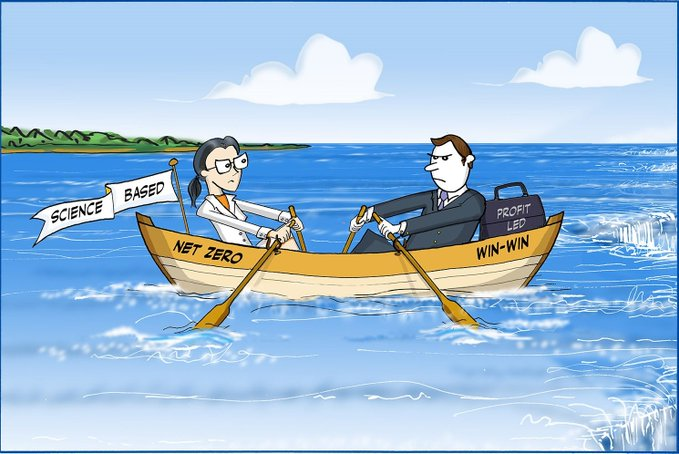
\includegraphics{fig/win-win_vs_net-zero.jpeg}

The challenge for the sustainable business community is that, as a market-based movement, it has generally not questioned `economic growth'. Sustainable business certainly espouses a preference for green growth, but that merely reinforces growth-favouring norms, with the consequence of waving through mostly non-green growth, at a time when environmental buffers are diminishing.

We are missing the physics for the finance. A major cause of our sustainability problems is that the economic values we steer by are so decontextualised from the underlying natural world that a core aspect of the sustainability challenge is to see through the blindness that economic and financial conventions induce.

Our ecological problems are rooted in matter and energy flows not financial flows. Our situation has arisen because we have transformed the matter and energy of the world at a much faster rate than the natural world can absorb. Given the entropic toll of every transformation, it is our underexamined urge to keep transforming -- even with good intention -- that is the core driver of our ecological crisis. But, in what sustainability researcher Pasi Heikkurinen has termed our `transformation paradox', our instinctive response to problems caused by past excess transformation of the world's matter and energy is to keep transforming! Our increasingly urgent ambition to build a green economy masks the deeper point that we remain firmly upon a transformation treadmill. We say `greener', the Earth just registers `more'.

In races against time, possibly the most precious commodity is more time. How can we buy time for our sustainability crisis? By slowing down those parts of the economy making no contribution to a greener future economy.

Critically, the de-growth or post-growth that advocates have in mind is not the sporadic recessions that upset our prevailing growth mindset, but rather an intentional, radical transformation and re-conception of prosperity and welfare, complete with transitional justice.

{[}Austin (2021) From Win-Win to Net-Zero{]}(\url{https://www.responsible-investor.com/articles/from-win-win-to-net-zero-would-the-real-sustainability-please-stand-up9}
\href{pdf/Austin_2021_Win-Win_Net-Zero.pdf}{(pdf full)}

\hypertarget{externalities-risks}{%
\section{Externalities Risks}\label{externalities-risks}}

\emph{Crona}

Globally, financial services are well positioned to contribute to the transformation needed for sustainable fu-
tures and will be critical for supporting corporate activities that regenerate and promote biosphere resilience
as a key strategy to confront the new risk landscape of the Anthropocene. While current financial risk frame-
works focus primarily on financial materiality and risks to the financial sector, failure to account for invest-
ment externalities will aggravate climate and other environmental change and set current sustainable finance
initiatives off course. This article unpacks the cognitive disconnect in financial risk frameworks between envi-
ronmental and financial risk. Through analysis of environmental, social, and governance ratings and esti-
mates of global green investments, we exemplify how the cognitive disconnect around risk plays out in
practice. We discuss what this means for the ability of society at large, and finance in particular, to deliver
on sustainability ambitions and global goals.

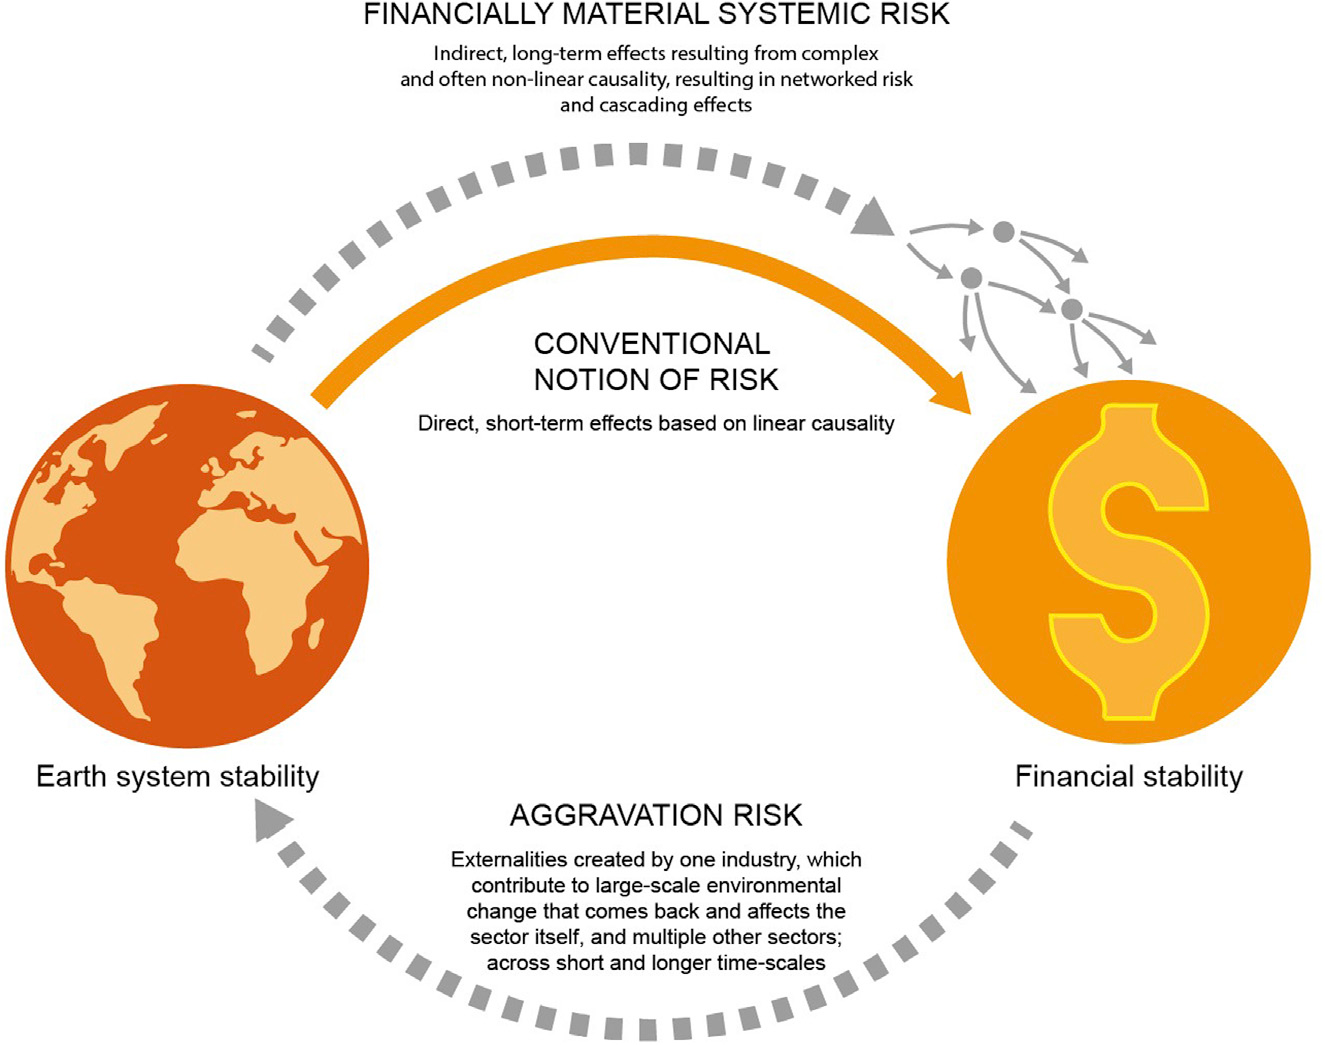
\includegraphics{fig/externalities_risks.png}

Global issuance of green bonds recently
surpassed \$250 billion, representing ca. 3.5\% of total global
bond issuance (\$7.15 trillion)

The multiple, often complex, mechanisms by which environmental change un-
folds and is aggravated by investments are not equally recognized.

Climate, biodiversity loss, water, and land-use change
are not isolated phenomena, but directly interconnected and
mutually reinforcing processes.

For example, deforestation to
produce oilseed in one region leads to regional drought affecting
the oilseed production itself, but also affecting geographically
distant sectors, such as aquaculture reliant on oilseed for
feed input.

Failure to see these connections matters. If they are not recog-
nized in risk assessment tools, strategies, and solutions used to
address the problem, these will deliver only partial results.

Most detrimental risks of climate change on portfolios may
very well arise from second-order effects.

This article contrasts widespread conceptions of climate-
related financial risks (such as those of the Taskforce on
Climate-Related Financial Disclosures {[}TCFD{]}) with insights
from Earth system science, to highlight the disconnect between
environmental and financial risk in prominent financial risk frame-
works. We show the necessity of a broader conceptualization of
climate and environmental risk to avoid devastating impacts on
the economy, society, and biosphere as a whole. We then use
environmental, social, and governance (ESG) investments as a
means to exemplify how the cognitive disconnect plays out in
practice and its implications for the ability for society at large,
and finance in particular, to deliver on sustainability ambitions
and global goals.

Multiple sources of scientific evidence show that a stable
climate is determined not just by GHG emissions, but by a com-
plex set of interactions between human activities and large-scale
biological, geological, and physical processes related to, e.g.,
forest and land-use dynamics, global hydrological flows, and
radiative forcing.

Climate stability hinges not just on the atmosphere.

Financial risk frameworks explicitly aimed at
incorporating climate systemic risk (e.g., Aglietta and Espagne) 40
fail to recognize that propagation mechanisms can also be linked
to interconnections between Earth system processes. They
consider merely social and economic elements.

Many disasters have happened because of a failure to imagine
that they were possible and therefore to build insurance to be
prepared.

The exceptional development in risk definitions in the financial
sector over the past 3 decades. A similar
trend is supported by the shifting focus of risk discussions in
the annual reports by the World Economic Forum. 55 This rapid
development in the definition of financially relevant risks shows
that a shift to also consider aggravation risk is possible

\emph{alfa and beta only}

Managing investment risk hinges on diversifica-
tion. Conventional portfolio risk management is limited to diver-
sifying idiosyncratic risk (managing alpha) by selecting securities
across different financial assets. It further assumes that this
diversification has no influence on market-wide issues that could
affect multiple asset classes (beta).

The assumption---that systemic risks affect
investments, but are not affected by these same investments---is
the single biggest theoretical failing of modern portfolio theory.

For large institutional investors and so-called ``universal
owners,'' with highly diversified and long-term portfolios repre-
sentative of entire capital markets, climate change has already
been recognized as a key driver of future value and not an exter-
nality.

Coalitions have therefore emerged to rally this highly
concentrated segment of the financial sector into action (see,
e.g., Climate 100+, with over 500 investors as signatories and
more than US\$47 trillion in assets under management), yet to
date these remain focused only on shifting away from fossil fuels
and do not consider the interconnected dynamics between eco-
nomic activity, Earth system dynamics, and biosphere resilience.

A 7-fold increase in claimed losses (from \$50 billion in 1980 to \$350 billion in 2017).

\emph{Crisis of insurablility}

As climate change-related risks, such as storms, fires, and
sea-level rise, all mount and occur simultaneously, the sheer vol-
ume of material assets affected and the multiple types of liabil-
ities incurred threaten to trigger a crisis of insurability.

Climate change will affect
many sectors simultaneously in the future. As such it will affect
financial institutions by reducing their capacity to diversify.

Most financial risk assessment
still relies on historical data, and would underestimate or
completely miss the potential for thresholds and cascading ef-
fects not previously experienced.

ESG frameworks are a good example of how the cognitive
disconnect plays out in practice. ESG refers to a collection of often
divergent approaches to using non-financial data for socially
responsible investment strategies. ESG grew out of a socially
responsible investment movement emerging as early as the
1960s, and early versions were motivated by a belief in sustainable
development, adopted a systems view, and focused on capturing
absolute assessments of corporate externalities. However, as
the interest in ESG issues rose in the wake of the 2004 UN Global
Compact report, the financial materiality-driven rationale was
favored by the major rating providers (such as MSCI). According
to Eccles et al., this was because such an approach was easier
to scale, was most closely aligned with investor needs for finan-
cially focused assessments, and also arguably did not challenge
investors to reflect on more complex externalities.
This way of conceptualizing ESG issues now dominates sus-
tainability approaches adopted by prominent norm-setting
actors such as the SASB, the TCFD, and the limited set of ESG
providers that hold the majority of market shares in the highly
concentrated market segment of ESG rating services.

Current ESG ratings are based on a risk
perception that does not account for externalities, and therefore
is unlikely to address the root causes undermining sustainability.

Divergence in ESG
ratings has spurred debates about what reliably constitutes a
sustainable investee, as it prevents comparison of the performance of ESG investments.

It runs an acute risk of developing sustainability strategies that are off the mark.

In systems science it is well
established that thresholds in systems are easily overshot
when feedback has long delays, leading to collapse.

Since shortening the time lag of how the Earth system operates
is not possible, two things will be key to achieve a financial
system that fundamentally promotes long-term sustainability:
(1) incorporating the necessary information feedback and
(2) developing structures by which this information is taken
into account and acted upon. The two cannot be treated in
isolation

In 2019 only 14\% of total global investments were linked to any form of ``green'' label.
While ``green'' or ``sustainability''-linked loans and bonds
have experienced significant growth, they represented less
than 0.5\% of total debt issued.

(32\%) of the \$95 trillion of total equity in 2019 were ``green.''

The bulk of green equity investments are in shares of
listed companies that were deemed to be associated with
any of the following procedures: positive, negative, or
norm-based screening; any type of ESG integration; sustain-
ability-themed (impact) investment; or engagement and
shareholder action. 85 Taken together these stretch ``sustain-
able investments'' to include a vast array of investment stra-
tegies with arguably very different capacities to achieve sus-
tainable outcomes.

As long as \emph{central banks} continue to
conceptualize prudential regulations as ``blunt instruments for
dealing with climate-related externalities,'' and maintain that
``adapting capital requirements to reflect externalities could
undermine their primary purpose, or give rise to undesirable
effects,'' it is questionable whether these efforts can become
little more than a rearranging of the proverbial deck chairs of
the ill-fated Titanic.

Mainstream approaches for delivering on sustainability ambitions (such as
ESG) are on a trajectory that is currently off the mark.

Refining ESG metrics without incorporating measures of impact
will increase precision, but fail to address accuracy.

Today, unintelligent
accountability appears to be rising in the financial sector, as a
result of misalignment between sustainability ambitions and current
risk frameworks and risk assessment measurements. This
hampers the crucial role finance can and needs to play.

Our analysis has highlighted three key actions that will sup-
port the financial sector in bridging this gap: (1) recognizing a
wider set of Earth system processes (including the climate
and hydrological flows in addition to GHGs); (2) acknowledging
that current risk frameworks lack an acknowledgment of the
risk of aggravating climate and large-scale environmental
change through investments; and (3) moving to develop impact
accounting systems that cut across all financial investments
and become a core part of capital allocation decisions. Doing
this will require forging new alliances between science and
finance, but also new transdisciplinary research to assist
finance in developing risk management tools to better address
the Anthropocene reality and ensure that the development of
impact accounting is grounded in both social and environ-
mental sustainability science.

\begin{verbatim}
Memo DH:
Giving up on Governments, appealing to finance
\end{verbatim}

\href{https://www.sciencedirect.com/science/article/pii/S2590332221002359\#undfig1}{Crona (2021) The Anthropocene reality of financial risk}
\href{pdf/Crona_2021_Anthropocene_reality_of\%20Financial_Risk.pdf}{(pdf)}
\href{pdf/Crona_2021_Anthropocene_reality_of\%20Financial_Risk_SI.pdf}{(pdf SI)}
\href{https://www.cell.com/one-earth/fulltext/S2590-3322(21)00235-9?_returnURL=https\%3A\%2F\%2Flinkinghub.elsevier.com\%2Fretrieve\%2Fpii\%2FS2590332221002359\%3Fshowall\%3Dtrue}{Alt link: One Earth}

\hypertarget{climate-impact-management-system}{%
\section{Climate Impact Management System}\label{climate-impact-management-system}}

\emph{2i Investing}

Recently, there has been a surge in financial sector initiatives focused on climate-related targets or strategies, with a number of big industry names making Net-Zero targets in the past few months alone.

However, some commitments have centered on targets that are decades away, with little clarity on the near-term actions that will be undertaken to meet these targets. Additionally, there has been limited focus on understanding how these kinds of initiatives will contribute to impact -- that is, greenhouse gas emissions reductions -- in the real economy (see our previous report, On the Road to Paris).

The Climate Impact Management System aims to fill this gap, by providing FIs with a clear roadmap to develop, refine, and communicate on impactful climate strategies. The system was developed by 2DII's Evidence for Impact Program and the French Ecological Transition Agency (ADEME), as part of the Finance ClimAct project.

\href{https://2degrees-investing.org/new-climate-impact-management-system-opens-for-consultation/}{2i Investing}
\href{pdf/Climate-Impact-Mgmt-System.pdf}{(pdf)}

\hypertarget{etf-universe}{%
\section{ETF Universe}\label{etf-universe}}

\emph{VisualCapitalist}

Globally, sustainable exchange-traded fund (ETF) assets hit \$150 billion last year, vaulting 25 times higher than in 2015.

Yet despite this growth, sustainable ETFs---baskets of investments that focus on environmental, social and governance issues---account for roughly 5\% of the entire ETF universe.

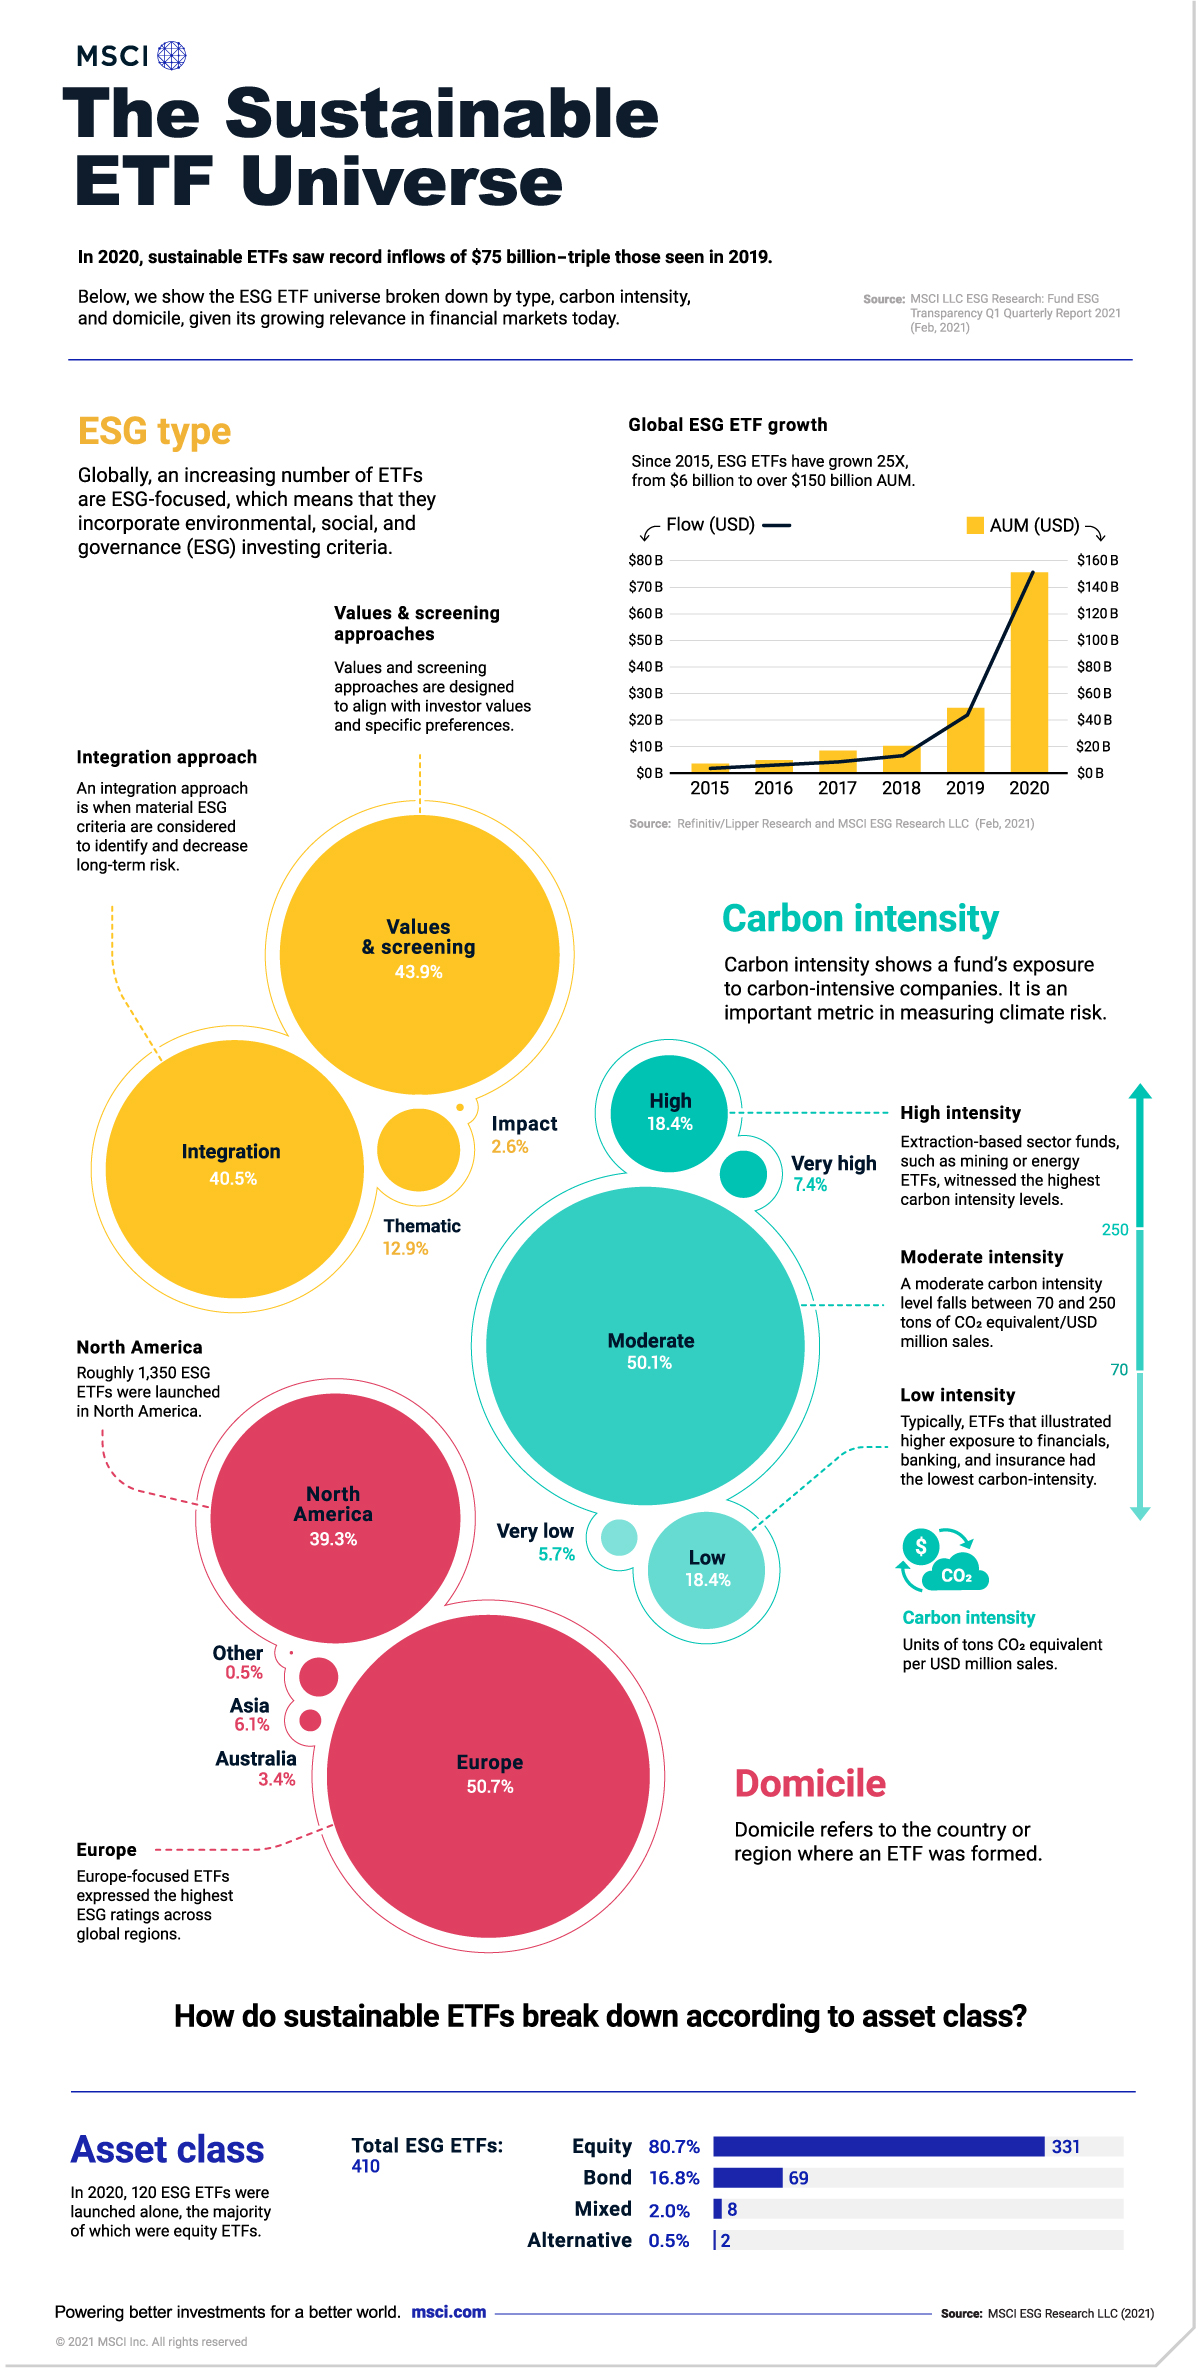
\includegraphics{fig/MSCI_Sustainable-Universe_210518.jpg}

\href{https://www.visualcapitalist.com/visualizing-the-sustainable-etf-universe/}{VisualCapitalist}

\hypertarget{fintech}{%
\chapter{FinTech}\label{fintech}}

\emph{Hendershott}

\textbf{FinTech has demonstrated tremendous power in fundamentally changing
how the financial market is run.}

Technologies have spawned finance innovations since the early days of com-
puter applications in businesses, most recently reaching the stage of disruptive innova-
tions, such as mobile payments, cryptocurrencies, and digitization of business assets. This
has led to the emerging field called financial technology or simply FinTech. In this editorial
review, we first provide an overview on relevant technological, pedagogical, and man-
agerial issues pertaining to FinTech teaching and research, with a focus on market trading,
artificial intelligence, and blockchain in finance. And then we introduce the articles
appearing in this special section. We hope that our discussions of potential research di-
rections and topics in FinTech will stimulate future research in the fields of information
systems and finance toward making their unique marks in the FinTech evolution and the
associated business and societal innovations.

\href{pdf/Hendershott_2021_FinTech_as_Game_Changer.pdf}{Hendershott (2021) FinTech as Game Changer}

\hypertarget{global-payment-infrastructure}{%
\chapter{Global Payment Infrastructure}\label{global-payment-infrastructure}}

\emph{Brandl Abstract}

Despite the narrative of a globalized economy, there is no effectively working global payment system. Although there is an infrastructure that allows the transmission of data about global payments, the movement of actual money is executed indirectly, making it an incalculable endeavor. The reason is that money is not simply data, but a complex bundle of rights closely tied to the nation state. In the absence of infrastructure that reliably links payments with guarantees of the nation state, intermediaries that facilitate global payments are forced to create trust in a different way. This is only possible by occupying a highly centralized and therefore powerful position. In this article, we investigate which actors were historically able to hold such a position and how these actors are challenged by digitalization. We suggest that there are three models of payment infrastructure provision. Bank-based systems were dominant until the 1980s, but in the following decades, a second model emerged: the provision of financial infrastructure by global companies. Since the early 2000s, we see a third model: the entrance of tech-driven companies in the payment sector. We conclude that digital technologies will not necessarily solve the problems, but might in fact exacerbate them.

\emph{Brandl Memo}

The difficulties in making cross-border payments leads us right into the heart of questions about the substance of modern money and the role of nation states in its production.
\href{https://www.tandfonline.com/doi/full/10.1080/09692290.2021.2016470\#}{Ingham (2004)} describes money as a private-public partnership. The object of this partnership is a constant struggle between three main groups of actors: governments, the people (the taxpayers), and rentiers and their banks. At the core of this conflict lies the question, `What counts as money at all?' since this question is crucial for the contemporary distribution of wealth

In this article, we claim that financial infrastructure is a mostly ignored2 but crucial component of the puzzle of `what counts as money', since only this infrastructure can execute the private-public partnership in everyday life. Such infrastructure ensures that the guarantees provided by the nation state in its own currency area are not mere promises; it links these promises to day-to-day payments in commercial bank money. This material underpinning linking payments with the promises of the nation state is absent in the global context and, therefore, cross-border payments have a very different nature than domestic payments.

Through the absence of infrastructure that reliably links payments with the guarantees of the nation state, intermediaries that facilitate global payments are forced to create trust in a different way. In this article we will show how these preconditions lead to the development of powerful intermediaries in the global payment industry that are able to dictate the conditions of cross-border payments.

Only through infrastructures can the promise of the nation state be linked across time and space.

Financial infrastructures might seem to be a monolithic bloc, they are actually provided by a broad range of actors and institutions. The main difference is between those focusing on the settlement of payments and those focusing on the settlement of securities.

The provision of infrastructures for payments, which is regarded as part of the critical infrastructure of a nation state equal to that of energy, water supply, food and agriculture, healthcare or transportation and is, therefore, closely linked to political regulation.

The expectation of the stability of the value of money has a temporal and a spatial dimension.

Money in capitalist societies is much more than data; it is a bundle of rights related to expectations about temporal and spatial value stability that are tied to guarantees provided by the nation state.

The generation of trust that ensures stable monetary value has at least two dimensions: temporal and spatial.

Scholars of economic history have extensively studied the establishment of national currencie. Four motivations drove the early nation states to create territorial currencies: (1) the creation and fostering of domestic markets; (2) the desire to control the domestic money supply; (3) the wish to link currency with fiscal policy; and (4) the strengthening of national identity. The process of the establishment of national currencies, however, did not go as smoothly as expected. The declaration of a currency as legal tender by a nation state does not preclude the existence of another currency. Consequently, currency or monetary pluralism is regarded not as an exception but as a characteristic of modern currency systems.

Alongside their critique of a single uniform national currency, anthropologists in particular have long studied the plurality of economic spheres and currencies and the difficulties of transferring values from one sphere to the other.
This is true not only for tribal society but also for modern capitalist societies.

Infrastructure: the link between the temporal and spatial dimensions of money.

One major component of the Fed was the establishment of the Gold Settlement Fund, which enabled the member banks to settle their reciprocal claims with central bank money. The costs of shipping gold between the various banks were reduced to zero, and therefore payments at par became possible.

Markets as one of the fundamental institutions of capitalism function precisely because fragmented actors come together to compete. However, these decentralized encounters are based on a (financial) infrastructure that must be as frictionless as possible, i.e.~centralized.

The first challenge in setting up financial infrastructure is consequently that competing companies must establish institutions that are able to uphold their trust in one another. Second, all actors involved must jointly provide the technological infrastructure capable of handling such a complex operation and enforce universal standards such as accounting systems. The problems that typically arise in this context are similar to those that generally come up in the provision of public goods: on the one hand, suboptimal incentive structures, which systematically lead to undersupply in the case of the private provision of a public good; and on the other hand, the occurrence of strong network effects which reinforce concentration tendencies.

Traditionally, the advice for industries with these tendencies has been that the state should be responsible for their provision. However, unlike other industries with a similar structure, such as telecommunication providers or providers of public utilities, the provision of financial infrastructure was only occasionally managed solely by the nation state.

why does the primarily private provision of infrastructure work in the finance sector, while it fails in other industries? One key reason for this might be that payment infrastructure can be provided as a club good such that non-paying actors can be excluded. It is important to understand that this `club' of commercial banks that provide infrastructure is deeply dependent on the close cooperation between private actors and state actors that provide oversight over the financial infrastructure as well as settlement infrastructures, which connect the privately provided infrastructures.

The private-public partnership that constitutes modern money is executed through public infrastructure, which is reliably linked to the infrastructure of networks of commercial banks. These infrastructures, which are run by central banks, are able to link day-to-day payments with the guarantees of the nation state by providing an infrastructure that allows banks to settle their reciprocal claims with central bank money.

The trust of all participants in payment infrastructures that emerge naturally in the domestic context is built on the basis of the fact that central bank money is the safest possible asset; for cross-border transactions this trust has to be produced by other means.

Clearing houses act as central counterparties (CCP), which means that they assume guarantees for their members in the event of default. To be able to do this properly, the clearing houses require large commitments from their members, usually in the form of reserves deposited with the central bank. In addition, the members are often subject to the regulations of the central counterparty (Interview 14). In this way, the central counterparties not only minimize the individual members' risk, but also reduce the systemic risk of the entire financial sector by homogenizing the individual credit risks, as all members are jointly liable for losses.

The transformation of one money into another money is not a simple and frictionless process. This is especially true for cross-border payments, since money is not only data but a bundle of rights that is tied to the guarantees of the respective nation state. This bundle of rights cannot be exchanged as such, since the essence of global transactions is that they leave the borders of the nation state. The only possibility is, therefore, that a powerful intermediary is able to bridge this gap.

Credit card companies, as well as other companies such as the Society for Worldwide Interbank Financial Telecommunication (SWIFT), do not supersede the nationally based infrastructures; rather, they are deeply dependent on them. SWIFT, a company that emerged from the association of commercial banks, provides an infrastructure for banks to send and receive messages about financial transactions.

Credit card companies provide international clearing arrangements, which means they provide the data that allows settlement, but the actual movement of money is carried out by a few major settlement banks. The role of these banks cannot be underestimated. For example, the entire settlement process for Visa (the largest credit card company) is done by Chase Manhattan Bank, which technically becomes a correspondent bank or handles the transactions through its subsidiaries.

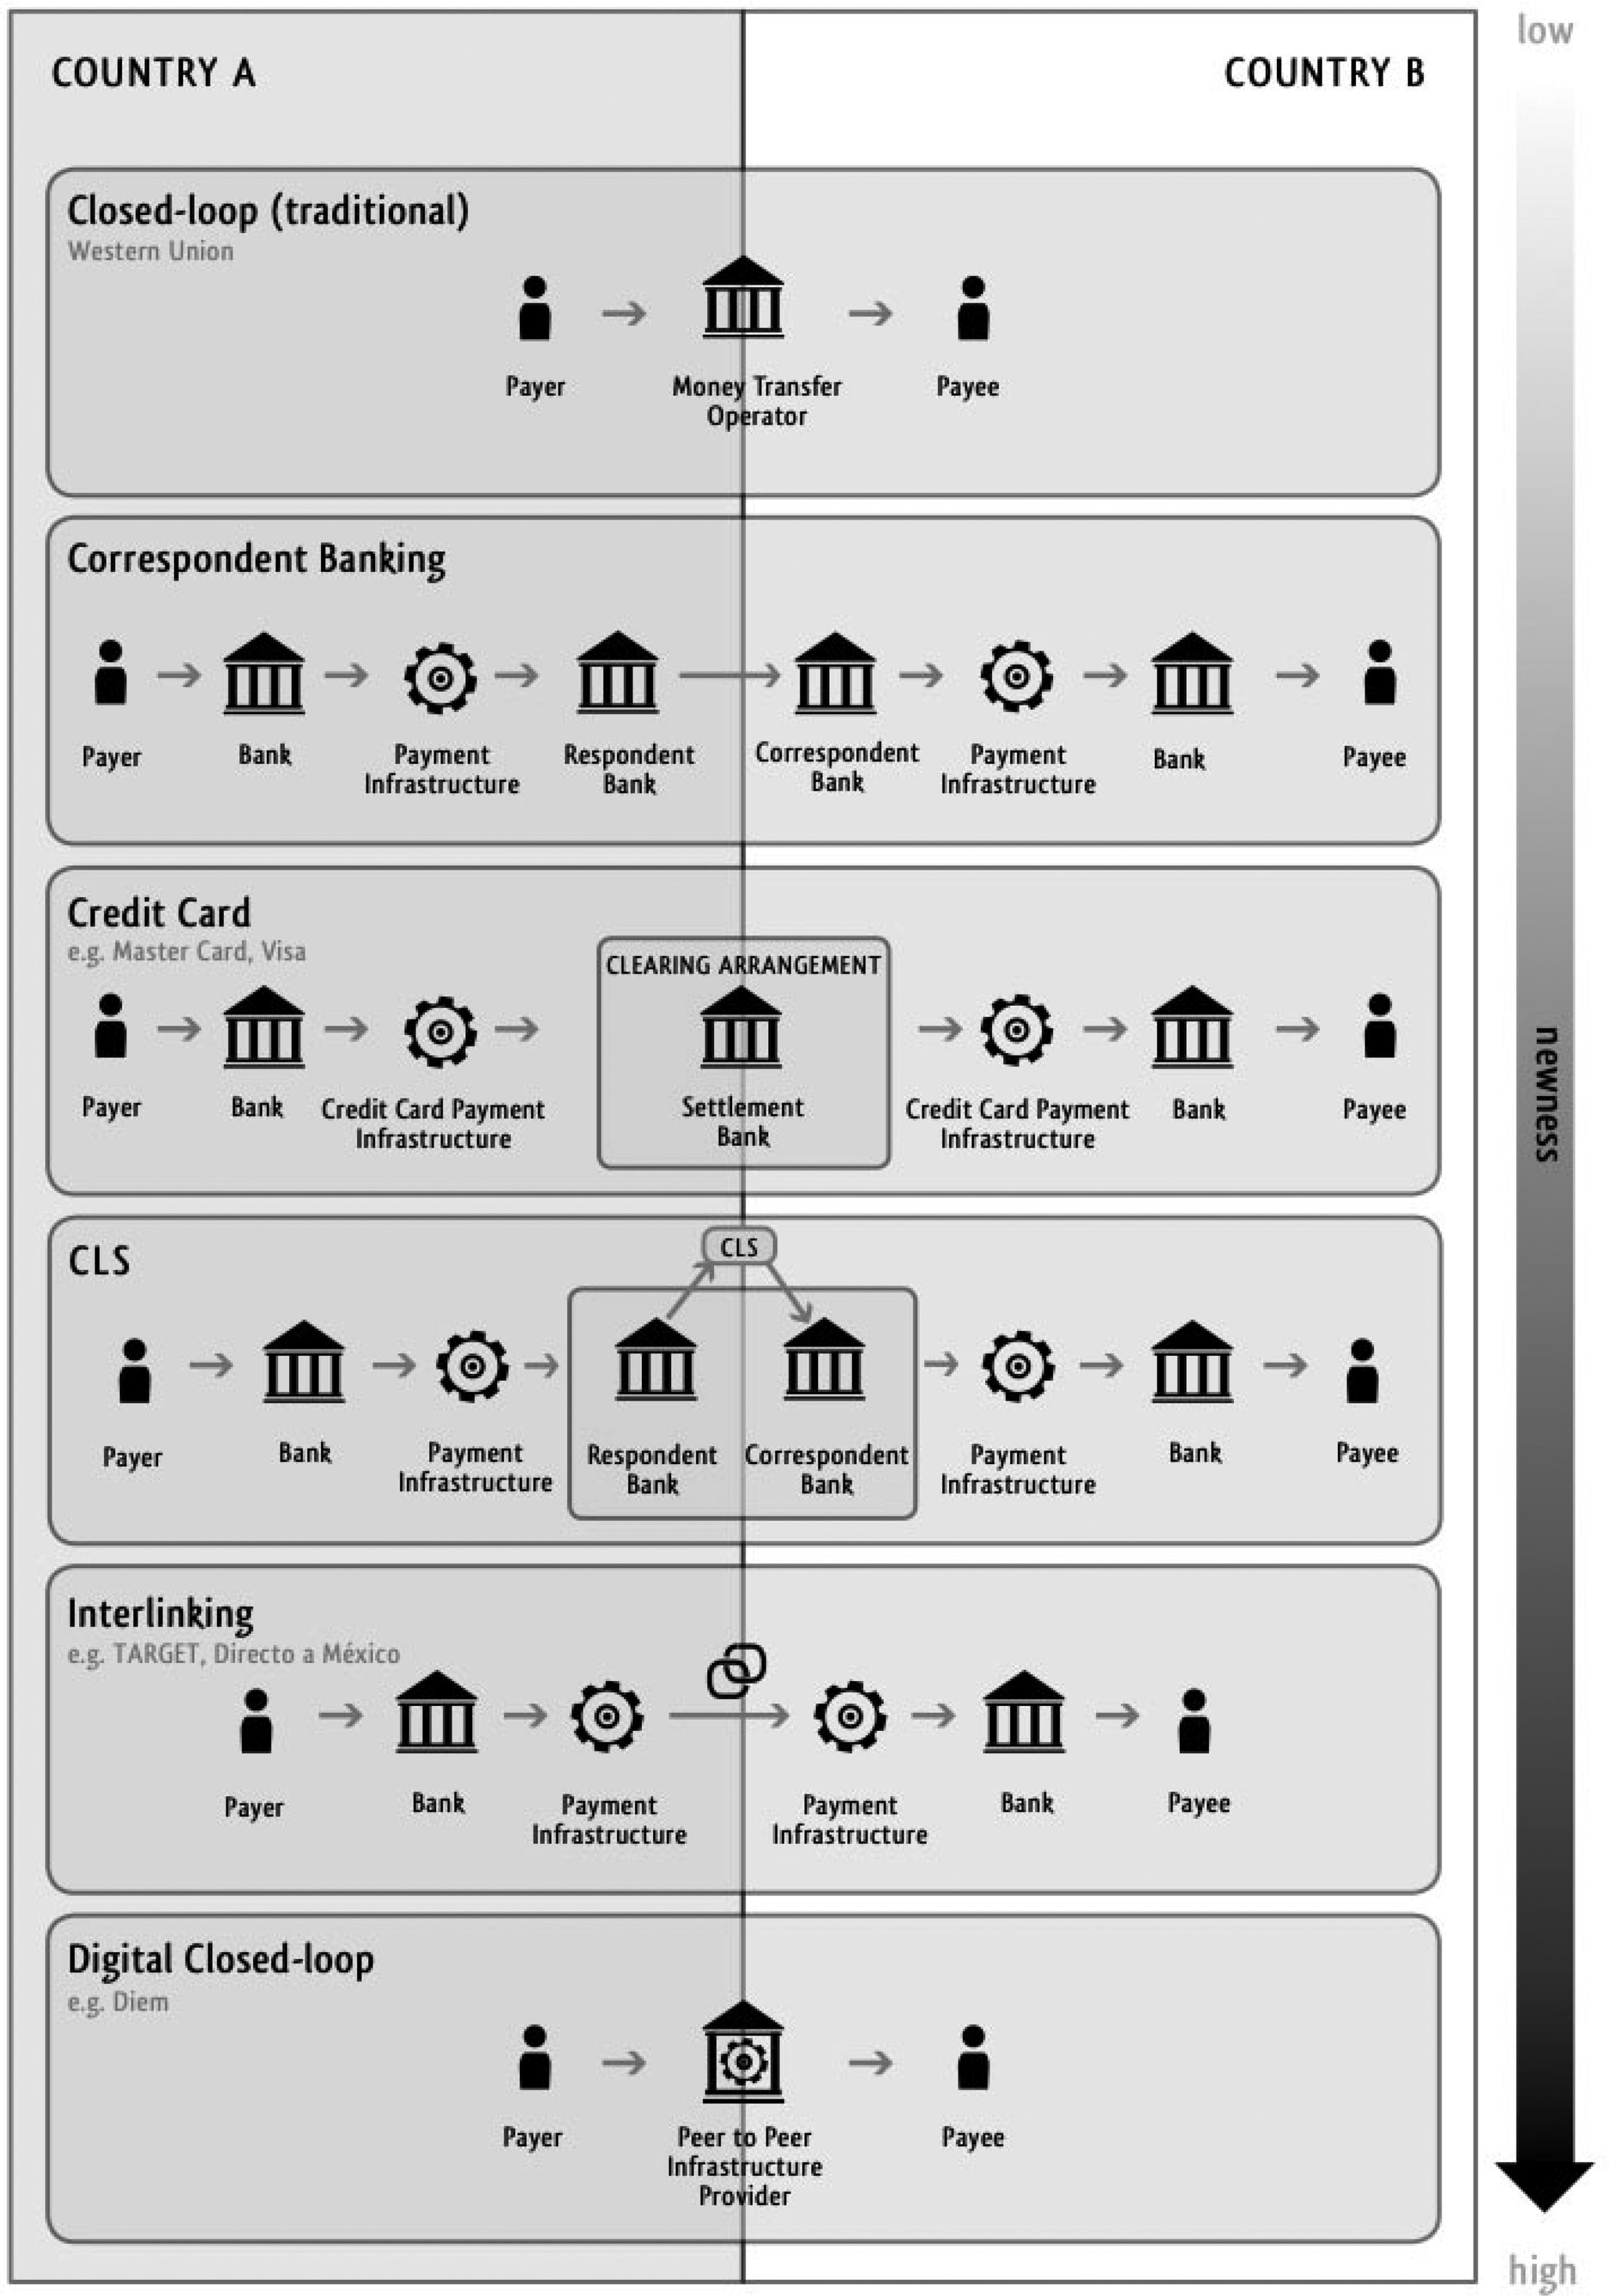
\includegraphics{fig/global_payment_processes.jpeg}

\emph{Figure: Cross-border Payments}

Banks handle their international transactions via correspondent banks or via their subsidiaries. Correspondent banking is a bilateral agreement between two banks in different countries by which one of them provides services to the other by holding an account (nostro or vostro account) owned by the respective other bank.
These agreements enable the respondent bank in Country A to participate in the payment systems of Country B. There are only a few major banks that provide these services globally.

while the settlement of domestic transactions is typically done with central bank money (the safest possible asset), the settlement of FX transactions involves commercial bank money.

The time lag between a currency payment and receipt of the currency being bought creates a risk exposure for the selling party: the risk that the delivery is late (liquidity risk) or in the worst case does not occur at all (credit risk). Although these types of risk also exist in domestic transactions, the risk that goes along with FX transaction settlements is higher.

This service comes with a price: the provision of infrastructure by an oligopoly of private companies.

Since the late 1990s, at least two innovations have enhanced the speed and lowered the cost of cross-border trades between the countries of the Global North. To reduce the risk exposure of cross-border payments, a network that consists of around 70 financial institutions established a settlement system (see Figure 1) for cross-border payments: CLS (continuous linked settlement). While the settlement provided by central banks is done with central bank money, the settlement in the CLS system is executed by the CLS Bank with a `payment vs.~payment' system that reduces the risk exposure for the involved parties. However, CLS only settles in 17 currencies8 of countries of the Global North as well as some emerging economies. FX transactions with minor or exotic currencies are still only possible via correspondent banks, and therefore even more incalculable and hence expensive.

Traditional closed-loop systems (or money transfer operators) such as Western Union have their own proprietary, quite opaque network of banks, exchange bureaus, post offices, and other intermediaries -- like retail outlets, cell phone centers, travel agencies, drug stores, and gas stations -- to deliver remittances.

In the Eurozone and a few other regions,10 we see a second innovation emerging from attempts by nation states to bridge the national financial infrastructures and build interlinking models (see Figure 1). In the context of the integration of the European capital market, one major step was the harmonization of the providers of financial infrastructure, which was done through TARGET 2 (Trans-European Automated Real-time Gross Settlement Express Transfer System) that was implemented between 2006 and 2017. The core of the Target system is a platform which allows all central banks of the euro system to settle their euro payments in real time. The Single Shared Platform is operated by the three major central banks: France (Banque de France), Italy (Banca d'Italia) and Germany (Bundesbank). Although the Bank for International Settlements (Bech et al., 2020) sees great promise for the interlinking model, global companies continue to dominate infrastructure provision.

In the European Union (EU), we see a massive regulatory push to disaggregate the value chain of the payment sector by promoting digital technology (Interviews 11 \& 16). This process is closely tied to the revision of the 2015 directive on payment services (PSD2), which aimed to open up the market for payment services. The core of this directive is that banks are required to grant other providers access to their customers' account data. As a result, the business models of the providers of digital payment systems were strengthened. The initial aim behind this initiative was to challenge the cartel of credit card companies from the European side (Stiefmüller, 2020). Guaranteed access to consumer data should foster competition in the market for payment services and should at best trigger the foundation of a European equivalent to PayPal. This initiative of the European Commission was almost exclusively motivated by competition law and supply-side concerns, but comes with a price tag: the limitation of data protection and the potentially related violation of privacy (Stiefmüller, 2020, p.~299). The exclusion of data protection concerns in the PSD2 directive is presumably due to fact that the EU regulators want to establish an economic area that can compete with the US to spawn innovation.

Both trends, the wave of digitalization in the financial sector and the regulatory push to promote these digital technologies, made the financial sector attractive for new types of players: startups and, of course, big tech companies such as Apple, Amazon and Facebook. The payment sector is particularly interesting for these companies because it produces highly attractive raw material: transactional data.

\emph{Platformization of financial transactions:} The big tech companies aim to integrate payment systems in their platforms to gain access to this highly valuable transactional payment data and to increase the time customers stay on their platforms. However, the key question is whether this development affects the oligopolistically provided financial infrastructure that now executes global payments.

The first company working this way on the front end was PayPal, founded in 1998.12 It was over a decade later when the large wave of startup formations in the payment sector began. As of 2021, the most successful actors in this field are startups such as Klarna or iZettle13 as well as the big tech companies that provide financial services such as Apple Pay and Google Pay.

We know from the example of the credit card companies that the market of payment providers develops strong network effects and, therefore, the further consolidation of the market is very likely.

In addition to tech-driven companies that provide financial services without becoming banks themselves, we can identify a second, much more radical strategy: the (almost) complete detachment of financial services from banks via the establishment of closed-loop systems. Although digital closed-loop systems emerged only recently, the principle is much older. More traditional remittance companies such as Western Union work on the same principle but require a physical presence in every jurisdiction. By contrast, digital closed-loop systems are based on digital currencies which are created by the networks themselves. The first attempt to establish such a digital closed-loop system for cross-border payments was made by Ripple. On the basis of distributed ledger technology14 Ripple creates its own currency (XRP), which is used for settlement.

Digital closed-loop systems are able to provide infrastructure that is able to move money. However, rather than actual currencies that are legal tender, these systems move their own digital currencies that eventually have to be exchanged in the currency of the respective country.

The risks associated with digital, proprietary closed-loop systems are evident. First, since these systems were established outside the highly regulated state--bank nexus, the lack of supervisory oversight might fail to identify shortcomings in risk management. The second concern is much more fundamental. Digital closed-loop operations may drive fragmentation through non-compatible payment systems within an economy.

While Ripple's ultimate goal is to revolutionize the global interbank market by convincing banks to join the Ripple network, we see initiatives from the big tech companies in the US to establish digital closed-loop systems for end users. In one of the best-known examples, Facebook founder Mark Zuckerberg announced plans to launch the digital currency Diem (originally called Libra) in cooperation with other companies.

Although Diem is based on a blockchain, it differs significantly from other cryptocurrencies such as bitcoin. In contrast to the majority of the existing cryptocurrencies, Diem is based on a permissioned blockchain, where only accepted members can participate. A second important difference is that the Diem blockchain does not create new value. Instead, the value on the Diem blockchain is fixed to that of existing currencies (so called stablecoins), and all values are fully backed by money that is deposited into Diem Reserve.
The Reserve exclusively relies on high-quality liquid assets or assets that can be easily converted into high-quality liquid assets.

Although China is outside of the scope of our analysis it is important to note that while most projects of western tech companies are still under development, these capabilities are already developed in China and other Asian countries. For example, a handful of companies in China, such as Alibaba's Alipay or Tencent's WeChatPay, provide digital infrastructures that link social media, commerce and banking, which work almost independently from banks. Next to these initiatives in the private sector, the efforts of China's central bank to provide a digital payment version of China's fiat currency -- the Renminbi -- are much further developed than comparable projects in the U.S. or Europe

The vast majority of attempts by tech-driven companies to transform the payment industry only affects the front end of banking and therefore leaves the role of major banks untouched.

The power of this club of major banks does not affect all actors in the same way. Powerful actors such as global companies are able to establish private solutions to bypass this problem via corporate treasury functions through their subsidiaries.

So far, digital technology, especially blockchain, has not challenged the concentration of power in only a few major players that are able to provide global financial infrastructure; instead it appears to strengthen existing intermediaries.

The resistance of the banking sector to disruptive changes driven by digital technology shows that the establishment of financial infrastructure is not as simple as the big tech companies might have thought. Banks and their organically grown infrastructures seem to have some advantages that cannot be easily copied by tech-driven companies. The reason for this might point to the characteristics of infrastructure, which are not purely technological arrangements, but as such evolving socio-technical systems which combine human and non-human elements for the provision of key functions in global finance.

\begin{quote}
Infrastructures are never neutral; they maintain the power relationships which are inscribed in their construction.
\end{quote}

\begin{quote}
Only powerful actors are able to build up enough trust to settle reciprocal claims with commercial bank money or, in the case of CLS and Ripple, with tokens they have created by themselves.
\end{quote}

The attempts of central banks to introduce digital central bank currencies might lead in the right direction. For example, the introduction of the Digital Euro might open up the possibility for participants outside of the EU to have access to central bank money. This would mean a big step in creating a global infrastructure that is actually able to move money and not only data. The consequences of an increase in euro-denominated assets outside of the EU, on the other hand, are completely unpredictable at this point. It is, therefore, not clear if this step is really desirable or whether it would ultimately break the exclusivity of the current infrastructure and make cross-border transactions more frictionless and less costly for everyone.

\href{https://www.tandfonline.com/doi/full/10.1080/09692290.2021.2016470}{Brandl (2021) The exclusive nature of global payments infrastructures: the significance of major banks and the role of tech-driven companies}

\hypertarget{imperialism-and-financialism-1}{%
\chapter{Imperialism and Financialism}\label{imperialism-and-financialism-1}}

\hypertarget{dollar-empire}{%
\section{Dollar Empire}\label{dollar-empire}}

\emph{Johnson Memo}

The world economy is structured by countries with competitive export sectors and trade surpluses, like Germany and China, who exhibit underconsumption and excess savings; the US's debt-fueled economy receives these savings through its domination of global financial markets. The dynamic strengthens the power of global finance at the expense of wages and living standards.

\href{https://phenomenalworld.org/analysis/reconstruction-finance}{Johnson}

\hypertarget{capital-as-power}{%
\section{Capital as Power}\label{capital-as-power}}

\emph{Bichler \& Nitzan Memo}

Over the past century, the nexus of imperialism and financialism has become a major axis
of Marxist theory and praxis. Many Marxists consider this nexus to be a cause of worldy
ills, but the historical role they ascribe to it has changed dramatically over time. The key
change concerns the nature and direction of surplus and liquidity flows. The first
incarnation of the nexus, articulated at the turn of the twentieth century, explained the
imperialist scramble for colonies to which finance capital could export its `excessive'
surplus. The next version posited a neo-imperial world of monopoly capitalism where the
core's surplus is absorbed domestically, sucked into a `black hole' of military spending
and financial intermediation. The third script postulated a World System where surplus is
imported from the dependent periphery into the financial core. And the most recent
edition explains the hollowing out of the U.S. core, a `red giant' that has already burned
much of its own productive fuel and is now trying to `financialize' the rest of the world in
order to use the system's external liquidity. This paper outlines this chameleon-like
transformation, assesses what is left of the nexus and asks whether it is worth keeping.

Our aim is to highlight the historical development of the
nexus of imperialism and financialism,
particularly the loose manner in which it has been altered --
to the point of meaning everything and nothing.

The paper comprises two parts. The first part examines the different schools. It
traces the transmutation of the nexus -- from its first articulation in the early twentieth
century, to the version developed by the Monopoly Capital school, to the arguments of
dependency and Word Systems analyses, to the thesis of hegemonic transition. The
second part offers an empirical exploration. Focusing specifically on the hegemonic
transition hypothesis, it identifies difficulties that arise when the theory meets the
evidence and assesses their significance for the century-old nexus.

\textbf{Empire and Finance}

The centralization of capital altered the political landscape. Instead of
the night-watchman government of the laissez-faire epoch, there emerged a strong, active
state.
The laissez-faire capitalists of the earlier era saw little reason to share their profits
with the state and therefore glorified the frugality of a small central administration and
minimal taxation. But the new state was no longer run by hands-off liberals. Instead, it was
dominated and manipulated by an aggressive oligarchy of `finance capital' -- a coalition of
large bankers, leading industrialists, war mongers and speculators who needed a strong
state that would crack down on domestic opposition and embark on foreign military
adventures.

The concentrated financialized economy, went the argument, requires pre-capitalist colonies
where surplus capital can be invested profitably; and the cabal of finance capital, now in
the political driver's seat, is able to push the state into an international imperialist
struggle to obtain those colonies.

At the time, this thesis was not only totally new and highly sophisticated; it also
fit closely with the unfolding of events. It gave an elegant explanation for the imperial
bellicosity of the late nineteenth century, and it neatly accounted for the circumstances
leading to the great imperial conflict of the first `World War'.

\textbf{Monopoly Capital}

In the brave new world of oligopolies, the emphasis on non-price competition
speeds up the pace of technical change and efficiency gains, making commodities cheaper
and cheaper to produce. But unlike in a competitive system, where market discipline
forces firms to pass on their lower costs to consumers, under the new circumstances, cost
reductions do not translate into falling prices. The prevalence of oligopolies creates a
built-in inflationary bias that, despite falling costs, makes prices move up and sometimes
sideways, but rarely if ever down.

This growing divergence between falling costs and rising prices increases the
income share of capitalists, and that increase reverses the underlying course of capitalism.
Marx believed that the combination of ever-growing mechanization and ruthless
competition creates a tendency of the rate of profit to fall. But the substitution of
monopoly capitalism for free competition inverts the trajectory. The new system
is ruled by an opposite `tendency of the surplus to rise'.

The early theorists of imperialism, although using a different vocabulary,
understood the gist of this transformation. And even though they did not provide a full
theory to explain it, they realized that the consequence of that transformation was to shift
the problem of capitalism from production to circulation (or in later Keynesian parlance,
from `aggregate supply' to `aggregate demand'). The new capitalism, they pointed out,
suffered not from insufficient surplus, but from too much surplus, and its key challenge
now was how to `offset' and `absorb' this ever-growing excess so that accumulation could
keep going instead of coming to a halt.

\textbf{Black Hole: The Role of Institutionalized Waste}

Until the early twentieth century, it seemed that the only way to offset the growing excess
was productive and external: the surplus of goods and capital had to be exported to and
productively invested in pre-capitalist colonies. But as it turned out, there was another
solution, one that the early theorists hadn't foreseen and that the analysts of Monopoly
Capital now emphasized. The surplus could also be disposed off unproductively and
internally: it could be wasted at home.

`Waste' denoted expenditures that are
necessary neither for producing the surplus nor for reproducing the population, and that
are, in that sense, totally unproductive and therefore wasteful. These expenditures absorb
existing surplus without creating any new surplus, and this double feature enables them to
mitigate without aggravating the tendency of the surplus to rise.

Use high military spending as a way to
secure the internal stability of U.S. capitalism.

The magnitude of military expenditures has no obvious ceiling: it
depends solely on the ability of the ruling class to justify the expenditures on the grounds
of national security. Similarly with the size of the financial sector: its magnitude expands
with the potentially limitless inflation of credit. This convenient expandability turns
military spending and financial intermediation into a giant `black hole'.

Spearheaded by U.S.-based multinationals and no longer hindered by inter-
capitalist wars, argued the theorists, the new order of monopoly capitalism has become
increasingly global and ever more integrated. And this global integration, they continued,
has come to depend on an international division of labour, free access to strategic raw
materials and political regimes that are ideologically open for business. However, these
conditions do not develop automatically and peacefully. They have to be actively
promoted and enforced.

Military spending comes to serve a dual role: together with the
financial sector and other forms of waste, it propels the accumulation of capital by black-
holing a large chunk of the economic surplus; and it helps secure a more sophisticated
and effective neo-imperial order that no longer needs colonial territories but is every bit
as expansionary, exploitative and violent as its crude imperial predecessor.

\textbf{Dependency}

The imperial powers relentlessly and systematically
undermined the socio-economic fabric of the periphery, making it totally dependent on
the core. And when decolonization finally started, the periphery found itself unable to
take off while the capitalist core prospered.
At that
point, there was no longer any need for core states to openly colonize and export capital
to the periphery. Using their disproportionate economic and state power, the former
imperialist countries were now able to hold the postcolonial periphery in a state of
debilitating economic monoculture, political submissiveness and cultural backwardness
-- and, wherever they could, to impose on it a system of unequal exchange.

This logic of dependent underdevelopment was first articulated during the
1950s and 1960s as an antidote to the liberal modernization thesis and its Rostowian
promise of an imminent takeoff.

Whereas earlier Marxist
theorists of imperialism accentuated the centrality of exploitation in production,
dependency and World-Systems analysts shifted the focus to trade and unequal
exchange. And while previous theories concentrated on the global class struggle,
dependency and World-Systems analyses spoke of a conflict between states and
geographical regions.

\textbf{Red Giant: An Empire Imploded}

`Financialization' is no longer a panacea for the
imperial power. On the contrary, it is a `sign of autumn', prime evidence of imperial
decline.

Finance (along with other
forms of waste) helps the imperial core absorb its rising surplus -- and in so doing
prevents stagnation and keeps accumulation going. But there is a price to pay. The
addiction to financial waste ends up consuming the very fuel that sustains the core's
imperial position: it hollows out the core's industrial sector, it undermines its productive
vitality, and, eventually, it limits its military capabilities. The financial sector itself
continues to expand absolutely and relatively, but this is the expansion of a `red giant' --
the final inflation of a star ready to implode.

The process leading to this implosion is emphasized by theories of hegemonic
transition.

The maturation of a hegemonic power -- be it Holland in the
seventeenth century, Britain in the nineteenth century or the United States presently --
coincides with the `over-accumulation' of capital.

This over-accumulation -- along with growing international rivalries,
challenges and conflicts -- triggers a system-wide financial expansion marked by soaring
capital flows, a rise in market speculation and a general inflation of debt and equity
values.
The financial expansion itself is led by the hegemonic state in an attempt to
arrest its own decline, but the reprieve it offers can only be temporary. Relying on finance
drains the core of its energy, causes productive investment to flow elsewhere and
eventually sets in motion the imminent process of hegemonic transition.

The United States benefited from being able to control,
manipulate and leverage this expansion for its own ends.
The growing severity of recent financial, economic and military crises suggests
that this ability has been greatly reduced and that U.S. hegemony is now coming to an end.

\textbf{End of Nexus?}

`Financialization' has not worked for the hegemonic power: despite the alleged
omnipotence of its Wall Street-Washington Complex, despite its control over key
international organizations, despite having imposed neoliberalism on the rest of the
world, and despite its seemingly limitless ability to borrow funds and suck in global
liquidity -- the bottom line is that the net profit share of U.S.-listed corporations has kept
falling and falling.

Of course, this isn't the first time that a monkey wrench has been thrown into the wheels
of the ever-changing nexus of imperialism and financialism. As we have seen, over the past
century the nexus has had to be repeatedly altered and transformed to match the
changing reality. Its first incarnation explained the imperialist scramble for colonies to
which finance capital could export its `excessive' surplus. The next version talked of a neo-
imperial world of monopoly capitalism where the core's surplus is absorbed domestically,
sucked into a `black hole' of military spending and financial intermediation. The third
script postulated a World System where surplus is imported from the dependent
periphery into the financial core. And the most recent edition explains the hollowing out
of the U.S. core, a `red giant' that has already burned much of its own productive fuel and
is now trying to `financialize' the rest of the world in order to use the system's external
liquidity.
Yet, here, too, the facts refuse to cooperate: contrary to the theory, they suggest
that the U.S. `Empire' has followed rather than led the global process of `financialization',
and that U.S. capitalists have consistently been less dependent on finance than their peers
elsewhere.

\href{http://bnarchives.yorku.ca/329/}{Bichler \& Nitzan (2012) Imperialism and Financialism}
\href{pdf/Bichler_Nitzan_2012_Imperialism_and_Financialism.pdf}{(pdf)}

\hypertarget{the-wall-street-consensus-1}{%
\chapter{The Wall Street Consensus}\label{the-wall-street-consensus-1}}

\begin{quote}
Washington Consensus and structural adjustment is good for you,
especially if it helps you avoid US bombing!
\end{quote}

\emph{Gabor}

The Wall Street Consensus is an elaborate effort to reorganize development interventions around partnerships with global finance. The UN's Billions to Trillions agenda, the World Bank's Maximizing Finance for Development or the G20's Infrastructure as an Asset Class update the Washington Consensus for the age of the portfolio glut, to `escort' global (North) institutional investors and the managers of their trillions into development asset classes. Making development investible requires a two‐pronged strategy: enlist the state into risk‐proofing development assets and accelerate the structural transformation of local financial systems towards market‐based finance that better accommodates portfolio investors. Ten policy commandments forge the `de‐risking state'. They create a safety net for investors in development assets, protecting their profits from demand risks attached to commodified infrastructure assets; from political risks attached to (progressive) policies that would threaten cash flows, including nationalization, higher minimum wages and, critically, climate regulation; and from liquidity and currency risks. These risks are transferred to the balance sheet of the state. The new `development as de‐risking' paradigm narrows the scope for a green developmental state that could design a just transition to low‐carbon economies.

\textbf{De-risking Wall Street}

\begin{quote}
`\ldots.we have to start by asking routinely whether private capital,
rather than government funding or donor aid, can finance a
project. If the conditions are not right for private investment, we
need to work with our partners to de-risk projects, sectors, and
entire countries'.
(Jim Yong Kim, World Bank Group President (2017))
\end{quote}

\emph{Washington Consensus}

\begin{quote}
Anchored in the work of John Williamson (1990, 1993),
the Washington Consensus outlined ten policy areas that would set countries on firm
market foundations, under a `holy Trinity' of macroeconomic \emph{stabilization} through
lower inflation and fiscal discipline; \emph{liberalization} of trade and capital flows, of
domestic product and factor markets; and \emph{privatization} of state companies.
\end{quote}

\emph{Financial globalization} sets the particular context in which
`international development' is pursued in the 21 st century.
The new development mantra, spelled out in the \emph{Billions to Trillions} agenda, the World
Bank's \emph{Maximising Finance for Development}, or the G20 \emph{Infrastructure as an Asset
Class}, aims to create investable development projects that can attract global investors
and orient their trillions into financing the SDG (Social Development Goals) ambitions.

For instance, at the 2017
launch of the Maximising Finance for Development, the World Bank promised global
investors \$12 trillion in market opportunities that include ``transportation,
infrastructure, health, welfare, education', minted into bankable/investible projects via
public-private partnerships (PPPs). These are long-term contractual arrangements
through which the private sector commits to finance, construct and manage public
services as long as the state, with multilateral development bank support via blended
finance, shares the risks to guarantee payment flows to PPP operators and investors.

This shift in the development agenda can be conceptualized as the Wall Street
Consensus, an emerging \emph{Development as Derisking} paradigm that reframes the (Post)
Washington Consensus in the language of the Sustainable
Development Goals, and identifies global finance as the actor critical to achieving the
SDG.

\emph{Financialisation of development} - strategies to `escort' financial capital
into derisked asset classes.

In the age of institutional investors
and asset managers that move capital across border via portfolio flows, (subordinated)
financialisation is no longer confined to the balance sheet of banks and non-financial
corporations, but becomes a state-mediated project of constructing new development
asset classes.

The WSC is an attempt to re-orient the institutional mechanisms of
the state towards protecting the political order of financial capitalism --
against climate justice movements and Green New Deal initiatives.

Development as derisking starts with the question `how to make projects bankable', or
how to construct investible development asset classes.

Making development `investible' requires a two-pronged strategy: (a) enlist the state
into derisking development asset classes, to ensure steady cash flows for investors and
(b) re-engineer local financial systems in the image of US market-based finance to
allow global investors' easy entry into, and exit from, new asset classes. Thus, Wall
Street Consensus marks a new moment in capitalist accumulation, from what David
Harvey (2003) termed `accumulation by dispossession' to accumulation by de-risking.

The state building project in the Wall Street Consensus is more ambitious than the Post-
Washington Consensus tolerance of the state as corrector of market failures, through
regulation and poverty alleviation (Öniş and Senses, 2005). The derisking state creates
a safety net for the holders of development assets, protecting their profits from demand
risks attached to infrastructure assets; from political risks attached to policies that would
threaten cash flows, including nationalization, higher minimum wages and, critically,
climate regulation; and from bond liquidity and currency risks. These risks are
transferred to the balance sheet of the state.

The practice of de-risking goes back to the developmental state, but its politics changed.
The developmental state `de-risked' domestic manufacturing in priority, mainly export,
sectors through industrial policies (Wade, 2018). It was successful where it had the
capacity to discipline local capital (Öniş, 1991), to govern market failures through
evolving institutional structures (Haggard 1990, 2018) and to generate elite support for
the developmental state as a political project (Mkandawire, 2001). In its modern
version, the entrepreneurial state adopts a ``mission-oriented'' market-shaping approach
that shares the risks and returns with highly-innovative private industries (Mazzucato
2016). In contrast, the WSC state de-risks development asset classes for global
institutional investors without the embedded autonomy of the developmental state
(Evans, 1991). It lacks an autonomous strategic vision, unless `more infrastructure' can
be described as such, and has fewer tools to discipline global finance.

The WSC downplays the risks of the macro-financial order it seeks to impose. It
engineers financial globalization that increases vulnerability to volatile capital flows.

In prioritizing market access, the Grand Bargain with private finance
protects bondholders from participating in debt renegotiations or debt service
suspension that poor and emerging countries require when under they come under the
pressure of large shocks such as the COVID19 pandemic or extreme climate events.
It threatens developmental policy space by narrowing the
scope for a green developmental state that could design a just transition to low-carbon
economies, where the burden of structural change does not disproportionately fall on
the poor.

If the Washington Consensus was a coordinated campaign for the global diffusion of
market-led policies, then the WSC coordinates a new modality of state governance
focused on derisking.

Development is narrated as a matter of closing funding gaps
through partnerships with (global) institutional investors,
while development interventions are defined as policies that
create risk buffers to render development projects `investible'.

The inclusion of institutional investors - from pension funds to insurance companies
and sovereign wealth funds -- and asset managers as critical stakeholders upgrades the
derisking renewables strategy into a full-blown, ambitious `development as derisking'
paradigm.
It reflects the political economy of macrofinancial reform in high-income countries
after the global financial crisis.

Worried primarily
by the `global banking glut', that is, excessive cross-border global bank
lending, high-income countries tightened global banking rules while simultaneously
promoting market-based finance, a `resilient' form of shadow banking dominated by
institutional investors and their asset managers. The growing footprint of these `new
powerbrokers of modern capital markets'
reflects the weakening capacity of the state to tax multinational corporations and high-
net worth individuals (that pour their cash into institutional investment vehicles) and to
provide traditional welfare to its citizens via public health, pensions, education
(prompting them to turn to asset-based welfare via pension funds and insurance
companies), often under the pressure of fiscal austerity discourses. These political
forces together have created a portfolio glut. Mirroring the `banking glut' of the pre-
2008 period of financial globalisation, generated by a handful of global banks, the
portfolio glut is also characterised unprecedented concentration of capital in the hands
of a few global asset managers such as Blackrock.

The \emph{portfolio glut} is studied in the capital flow management literature
through Rey's (2015) global financial cycle, the idea that
financial globalisation creates a trade-off between monetary policy autonomy and free
capital flows, rendering middle-income and poor countries vulnerable to US dollar
financing conditions.

It creates demands for a new \emph{`derisking' mode of governance} for states in the Global South.

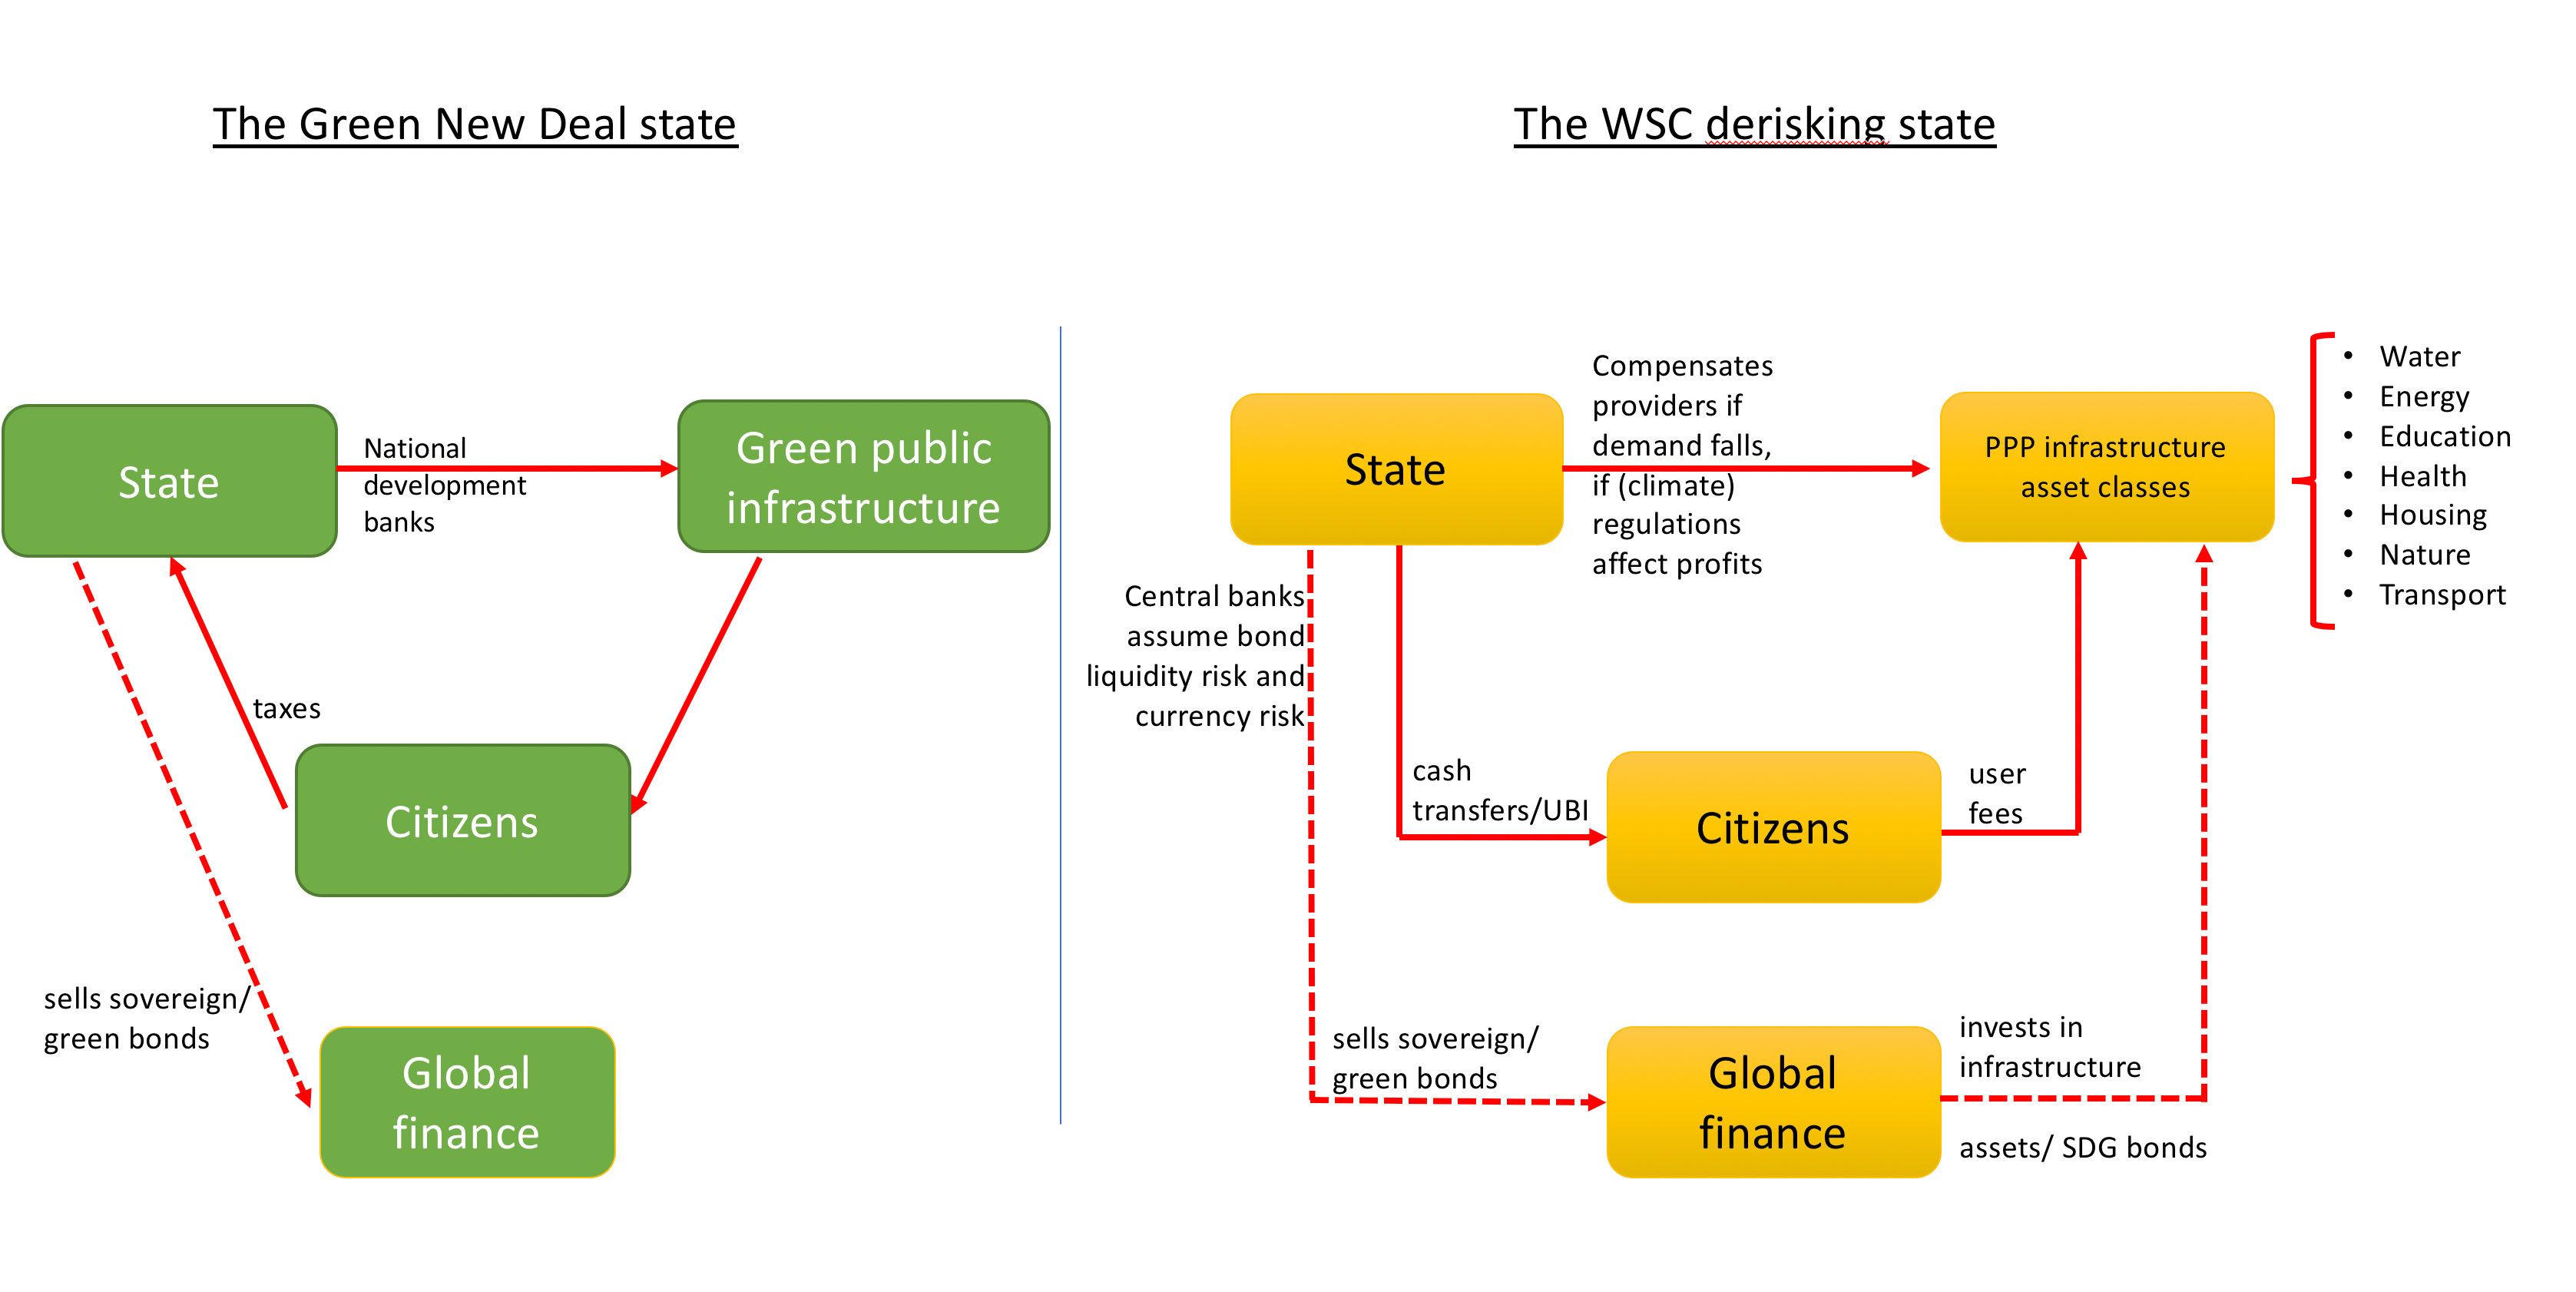
\includegraphics{fig/WSC_State.png}

In the derisking mode of governance, the state designs a menu of sector-specific policy
and financial derisking measures to encourage PPPs, accepts that this involves the
commodification of infrastructure via user-fees but puts in place cash
transfers/universal basic income schemes to mitigate the potential exclusion of the poor
from these services. That the derisking state does distributional politics through cash
transfers paradoxically accommodates calls for rethinking welfare politics as wage
labour becomes increasingly precarious.
Cash transfers enable the poor to access commodified public services,
and where these are not large enough, the state steps in to guarantee cash flows to investors.

Thus, development is not simply one-side defined by the political economy of capital,
but more specifically, by financial capital seeking to expand to new
areas, for which it colonises the infrastructure of the state. Financial capital no longer
just drags the poor into the embrace of the market, but also the state.

The derisking state can thus be understood as a project that seeks to extend the
infrastructural dependence of the state on finance -- and thus the infrastructural power
of the latter -- from its two traditional domains of monetary and fiscal policy to other
arenas of the government.

Derisking is not just about the transfers of risks to the state.
It is also about exercising infrastructural power to prevent
(regulatory) risks from materialising.

Derisking involves the central bank taking on its balance sheet bond liquidity and
currency market risks.

The legal battles to code capital into development asset
classes requires the state to take risks from the private sector onto its balance sheet, in
a clandestine reorienting of public resources that maintains the ideological commitment
to `fiscal responsibility'.

The WSC state assumes demand risk in user-fee based (social) infrastructure and
political risk that future governments might (re-)nationalize commodified
infrastructure or introduce tighter regulations, ranging from labour laws to climate
regulations that would affect profitability.

Uruguay's PPP law, passed by the
Mujica government in 2011, caps the total direct and contingent liabilities generated by
PPPs for the state to 7\% of the previous year's GDP, and fiscal transfers to private
operators to 0.5\% of previous year's GDP.

The fiscal costs of protecting investors from demand volatility will rise rapidly as
extreme climate events accelerate. Indeed, the climate crisis creates political and
demand risks that institutional investors need de-risking for.

The WSC protects investors against the political risks associated with green
developmental states. The green developmental state would prioritise the reorientation
of finance towards low-carbon activities. This requires a public taxonomy of green/dirty
assets that overcomes the shortcomings of private ESG ratings, and policies to penalize
dirty assets (through capital requirements or haircuts) 21 . Yet in the Wall Street
Consensus framework, such policies would classify as political risks, and require the
state to compensate their holders.

In its strategy to mutate climate risks into political and demand risks, private finance
may have found an important ally. Central banks conceptualize the immediate impact
of tighter climate rules regulation that increase the cost of funding or dramatically
change asset values as \emph{transition risks}.
The faster the low-carbon
transition, it is argued, the higher the potential that transition risks affect financial
stability, thus binding central banks in political trade-offs that privilege incremental
green regulatory regimes and accommodate greenwahing, however urgent the climate
crisis. Indeed, when central banks prioritize transition risks, they effectively rely on
private finance to drive the climate agenda, with their coordinating role focused on
subsidizing green assets, via so-called `green quantitative easing'.

In seeking to enlist central banks in the political coalitions against biting climate
regulation, the Wall Street Consensus constrains the green developmental states
directly, by making it liable for transition risks that can be framed as political and
demand risks, and indirectly, by reducing the public resources and central bank support
for Green New Deal programs that can effectively manage transition risks. The de-
risking state and the green developmental state can hardly co-exist, particularly within
market-based financial structures.

\textbf{Derisking market-based finance (formerly known as shadow banking)}

The turn to private finance as vehicle for sustainable development requires a change in
financial structures to accommodate the portfolio glut. It makes shadow banking,
understood as the production (via securitization) and financing (via wholesale funding
and derivative markets) of tradable securities, the desirable structure for financial
systems across the Global South. Indeed, the WSC consolidates
several global initiatives to restructure bank-based financial systems into market-based
finance or shadow banking,
where institutional investors can easily purchase local bonds (securities), including
infrastructure-backed securities, and finance as well as hedge their securities positions
via repos and derivative markets. Structural policies shift from developmental states'
concern with the productive structure, to the financial system.

The Financial Stability Board announced in 2015 that its new priority would be to transform
shadow banking into resilient market-based finance, which it defined as securities,
derivatives and repo markets.

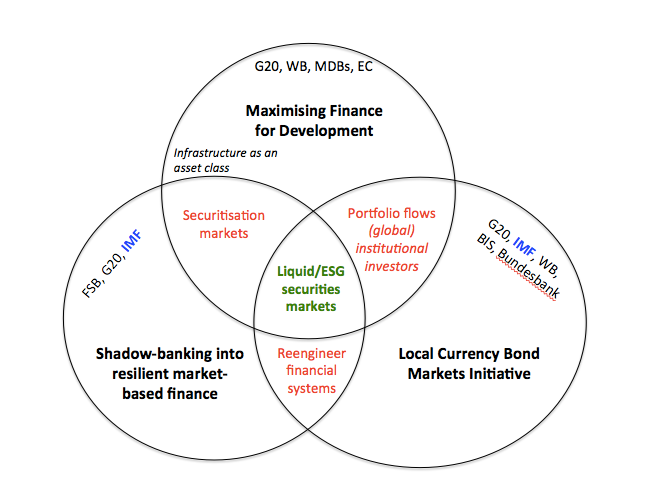
\includegraphics{fig/new_development_finance.png}

Figure: The turn to securities markets/market-based finance in international development

In sum, the organizational promoters of the Wall Street
Consensus championed in a multiplicity of global regulatory spaces the idea that
financial structure change is critical to attract the portfolio glut.

The
securitization of infrastructure loans would create both highly rated, low-return
tranches suitable for conservative pension funds/asset managers and lower-rated,
higher return tranches suitable for risk-driven investors. It would also accelerate lending
to infrastructure projects, constrained by Basel III rules for banks.

Since market-based finance is more systemically vulnerable than traditional bank-based
systems, the Wall Street Consensus assigns a triple de-risking role to central banks: in
bond markets and currency markets as market-makers of last resort,
and, forced by the inevitable consequences of green washing, as climate rescuers of last
resort, for assets left devalued by extreme climate events.
Some derisking
interventions, particularly in government bond markets, are at odds with the ideological
premises of central bank independence. Thus, the process of implicating central banks
in upholding the institutional basis of the derisking-centred accumulation regime is
incremental. It builds on crises such as the COVID19 pandemic to normalize new
derisking practices.

Greenwashing, like any
other regulatory arbitrage, eventually confronts its architects with the systemic
problems it feeds -- extreme climate events will devalue carbon-intensive assets and
greenwashed assets. The political logic of the Wall Street Consensus calls for central
banks to rescue the holders of last resort for carbon-intensive assets (Jahnke, 2019), to
risk-proof their portfolios, taking on its balance sheet the consequences of systemic
greenwashing.

`Development aid is dead, long-live private finance!'

\emph{Conclusion}

The Wall Street Consensus re-imagines international development interventions as
opportunities for global finance. In the new `development as derisking' paradigm,
institutional investors and asset managers are able to influence, if not altogether shape,
the terms on which poor countries join the global supply of `SDG' securities.
Multilateral development banks lead the efforts to design the ``de-risking''/subsidies
measures that seek to protect global investors from political risk or the demand risk
associated with privatized public services.

Equally important, this is a state-building project that puts in place the institutional
basis for a new regime of derisking as accumulation. The state comes under pressure
to institutionally codify risk-proofing arrangements, guaranteeing private financial
profits in the name of aligning sustainable projects with the preferred risk/return profile
of institutional investors. This includes adopting the US model of private pensions and
insurance to create local institutional investors. The tendency toward concentration in
the asset management sector (to exploit economies of scale and scope) may result in
Global North asset managers absorbing the funds of poor countries' institutional
investors and making allocative decisions on a global level.

In pushing for financial system change, development as derisking threatens to render
obsolete the old developmental banking model that put finance in the service of well-
designed industrial strategies. Development banks join the efforts of constructing and
derisking development asset classes. This is a political choice. Developmental banking
can arguably better serve a sustainability agenda because banks can easier include,
monitor and enforce safeguard policies in long-term relationships with customers. Most
countries with a successful experience of industrialisation relied on public development
banking as a critical pillar of industrial policies (Naqvi et al, 2018). Public development
banking allowed the developmental state to derisk via long-term loans to industrial
sectors identified as strategic by an industrial policy aimed at promoting the
international competitiveness of local firms.

This re-engineering of financial systems in the Global South, threatens the space for
alternative development strategies, and for a green developmental state. Government
capacity to design autonomous policies, in many poor countries severely eroded by
structural adjustment, will be further eroded by pressures to allocate scarce resources
to creating the conditions for private development finance.

\href{https://onlinelibrary.wiley.com/doi/abs/10.1111/dech.12645}{Daniela Gabor (2021) The Wall Street Consensus (Paywall)}
\href{pdf/Gabor_2021_Wall_Street_Consensus.pdf}{Draft (pdf)}

\hypertarget{part-appendices}{%
\part{Appendices}\label{part-appendices}}

\hypertarget{appendix-appendices}{%
\appendix}


\hypertarget{about}{%
\chapter{About}\label{about}}


\includegraphics{fig/me.jpg}

\emph{Dyre Haugen} and \emph{Dyrehaugen} is Webian for \emph{Jon Martin} -
self-owned Globian, Webian, Norwegian and Canarian with
a background from industrial research policy, urban planning and
economic development consulting on global, regional and urban scales.
I am deeply concerned about the (insane) way
humanity (i.e.~capitalism) interfere with nature.
In an effort to gain insights in how and why this happens
stuff is collected from around the web and put together
in a linked set of web-sites.
The sites are operated as personal notebooks.
However, these days things can be easily published to the
benefit of others concerned with the same issues.
But be aware - this is not polished for presentation or
peer-reviewed for exactness.
I offer you just to have a look at my `work-desk' as it appears in the moment.
Any comment or suggestion can be mailed to \href{mailto:dyrehaugen@gmail.com}{\nolinkurl{dyrehaugen@gmail.com}}
You can follow me on twitter as @dyrehaugen.
Thanks for visiting!

\hypertarget{links}{%
\chapter{Links}\label{links}}

\textbf{Current Dyrehaugen Sites:}

\begin{itemize}
\tightlist
\item
  \href{https://dyrehaugen.github.io/rcap}{rcap - On Capitalism} \href{http://localhost/rcap}{(loc)}
\item
  \href{https://dyrehaugen.github.io/rclm}{rclm - On Climate Change} \href{http://localhost/rclm}{(loc)}
\item
  \href{https://dyrehaugen.github.io/recs}{recs - On Economics} \href{http://localhost/recs}{(loc)}
\item
  \href{https://dyrehaugen.github.io/rngy}{rfin - On Finance} \href{http://localhost/rfin}{(loc)}
\item
  \href{https://dyrehaugen.github.io/rngy}{rngy - On Energy} \href{http://localhost/rngy}{(loc)}
\item
  \href{https://dyrehaugen.github.io/renv}{renv - On Environment} \href{http://localhost/renv}{(loc)}
\item
  \href{https://dyrehaugen.github.io/rsts}{rsts - On Statistics} \href{http://localhost/rsts}{(loc)}
\item
  \href{https://dyrehaugen.github.io/rurb}{rurb - On Urbanization} \href{http://localhost/rurb}{(loc)}
\item
  \href{https://dyrehaugen.github.io/rvar}{rvar - On Varia} \href{http://localhost/rvar}{(loc)}
\item
  \href{https://dyrehaugen.github.io/rwsd}{rwsd - On Wisdom} \href{http://localhost/rwsd}{(loc)}
\end{itemize}

\textbf{Blogs:}

\begin{itemize}
\tightlist
\item
  \href{https://dyrehaugen.github.io/rde}{rde - Blog in English} \href{http://localhost/rde}{(loc)}
\item
  \href{https://dyrehaugen.github.io/rdn}{rdn - Blog in Norwegian} \href{http://localhost/rdn}{(loc)}
\end{itemize}

\textbf{Discontinued:}

\begin{itemize}
\tightlist
\item
  \href{https://dyrehaugen.github.io/jdt}{jdt - Collection (Jekyll)} \href{http://localhost/jdt}{(loc)}
\item
  \href{https://dyrehaugen.github.io/hdt}{hdt - Collection (Hugo)} \href{http://localhost/hdt}{(loc)}
\end{itemize}

\textbf{Not listed:}

\begin{itemize}
\tightlist
\item
  (q:) dhe dhn jrw56
\item
  (z:) rcsa rpad rstart
\end{itemize}

\hypertarget{news}{%
\chapter{NEWS}\label{news}}

\hypertarget{occ-nominee-fight}{%
\section{211118 OCC Nominee fight}\label{occ-nominee-fight}}

\emph{The Prospect}

\begin{quote}
``She does not see banks as the clients of the OCC.''
\end{quote}

After several months, President Biden has finally chosen a nominee to head the Office of the Comptroller of the Currency (OCC), a key financial regulatory post. It's Saule Omarova, a Cornell professor and critic of financial overreach.

Omarova immediately faced a flood of criticism from the banking industry, described as ``radical'' and ``Biden's most polarizing pick for a top financial regulatory job.''

Thus far, Omarova has been primarily condemned for musing in an academic paper last year about how individual bank accounts at the Federal Reserve could replace private deposits. The U.S. Chamber of Commerce on Tuesday announced their ``strong opposition'' to Omarova for precisely this reason.

THE CHOICE OF OMAROVA breaks sharply with precedent for the traditionally bank-friendly office. Established by Abraham Lincoln as a branch of the Treasury in 1863, the OCC is the main regulator for federally chartered banks, overseeing roughly two-thirds of total assets in the U.S. banking system. The agency is self-financed through the inspection fees it charges the banks it oversees, a funding mechanism critics of deregulation have identified as a conflict of interest.

The history of the OCC over the past half-century gives those critics abundant evidence that the agency operates as a bank advocate masquerading as a prudent regulator.

\href{https://prospect.org/economy/wall-streets-attacks-on-biden-nominee-red-herring-saule-omarova/}{The Prospect (2021) Wall Street's Attacks on Biden Nominee Are a Red Herring}

\hypertarget{gfanz-low-carbon-banking}{%
\section{210421 GFANZ: Low Carbon Banking}\label{gfanz-low-carbon-banking}}

Banks and financial institutions with more than \$70tn assets have pledged to cut their greenhouse gas emissions and ensure their investment portfolios align with the science on the climate.

In the initiative, chaired by Mark Carney, the former governor of the Bank of England, 160 companies, including 43 banks from 23 countries, will set targets to cut the carbon content of their assets by 2030, in line with an overall goal of net zero emissions by 2050.

The forum, the \emph{Glasgow Financial Alliance for Net Zero}, aims to encourage the financial sector to divert investment towards low-carbon infrastructure and technologies, and to discourage high-carbon investments, ahead of Cop26, the vital UN climate talks to be hosted by the UK in Glasgow this November.

Janet Yellen, the US Treasury secretary, and John Kerry, the US special presidential envoy for climate, are backing the alliance.

GFANZ {[}will be{]} the gold standard for net zero commitments in the financial sector.
The alliance would not allow banks to ``greenwash'' their commitments.

However, since the signing of the Paris agreement in 2015 banks have poured at least
\href{https://www.theguardian.com/environment/2021/mar/24/big-banks-trillion-dollar-finance-for-fossil-fuels-shocking-says-report}{\$3.8tn into fossil fuel financing}.

The financial system is fuelling environmental breakdown on a catastrophic scale, and what we really need is for central banks to play their roles as regulators and take concrete action to prevent all of the firms they oversee from making investments that are incompatible with governments' climate targets.

Banks signing up to GFANZ would be required to show ``credible plans'' for reducing their investment in high-carbon assets, but would not face a deadline for exiting fossil fuel investment.
Advertisement

Officials said there would be no blanket requirements for companies to stop financing coal, for instance, and banks would be allowed to make their own judgments on the carbon content of their portfolios, on a case by case basis.

\href{https://www.theguardian.com/business/2021/apr/21/leading-finance-firms-sign-up-to-mark-carney-forum-on-low-carbon-investment}{Guardian}

\hypertarget{biodiversity-and-financial-stability}{%
\section{210406 Biodiversity and Financial Stability}\label{biodiversity-and-financial-stability}}

\textbf{NGFS and INSPIRE launch a joint research project on `Biodiversity and Financial Stability'}

A growing number of central banks and supervisors have recognised the need to extend their focus from climate change to the challenges of addressing the implications of broader nature-related risks and the conservation of nature and biodiversity. Doing this will involve understanding the impact of finance on the provision of key ecosystem services as well as the consequences of biodiversity loss for financial stability.

Companies are highly dependent on the services that ecosystems provide, but may at the same time have a harmful impact on the environment. The financial risks that stem from a loss in biodiversity are a serious threat to the financial sector that urgently require better understanding by policy makers and regulators to which the new NGFS/INSPIRE Study Group will provide an important contribution.

  \bibliography{book.bib,packages.bib}

\end{document}
